\documentclass[10pt,twocolumn,letterpaper]{article}

% ---- arXiv-preprint style, pdflatex ----
\usepackage[letterpaper,top=2.2cm,bottom=2.4cm,left=1.8cm,right=1.8cm,columnsep=0.65cm]{geometry}
\usepackage{mathptmx}            % Times text+math
\usepackage[T1]{fontenc}
\usepackage[utf8]{inputenc}
\usepackage{microtype}
\usepackage{graphicx}
\usepackage{booktabs}
\usepackage{multirow}
\usepackage{amsmath,amssymb}
\usepackage{xcolor}
\usepackage[font=small,labelfont=bf]{caption}
\usepackage{subcaption}
\usepackage[numbers,sort&compress]{natbib}
\usepackage{titlesec}
\usepackage{placeins}
\titlespacing*{\section}{0pt}{1.1em}{0.5em}
\titlespacing*{\subsection}{0pt}{0.9em}{0.4em}
\usepackage[colorlinks=true,linkcolor=blue!60!black,citecolor=blue!60!black,urlcolor=blue!60!black]{hyperref}

\newcommand{\model}{Qwen-Image-Edit-2511}
\newcommand{\eg}{\emph{e.g.}}
\newcommand{\ie}{\emph{i.e.}}

\title{\LARGE\bf Supplementary Material\\[4pt]
\Large When Does an Image Edit Become Predictable? A Layer--Time Lens for Diffusion Editors}

\author{Anonymous Submission}
\date{}

\begin{document}
\raggedbottom
\twocolumn[
  \maketitle
  \begin{center}\begin{minipage}{0.92\textwidth}
  \small
  \textbf{Abstract.}
  We build a layer--time and tuned lens for a 60-block
  diffusion-transformer image editor, decoding intermediate residual
  streams through its frozen output head and pairing passive readings
  with generation-level probes and interventions. Under a fixed source
  and underspecified recoloring prompt, early states predict the final
  seed-conditioned outcome: the original car probe reaches 0.667
  balanced accuracy against 0.333 chance, and a pre-registered
  natural-photo tree replication reduces hue error from
  $55.9^\circ$ to $11.4^\circ$. As a held-out behavioral test, early
  best-of-five selection works on both Qwen and an independent 40-block editor, reducing
  measured compute by about 68\%. In Qwen, the target-image code remains
  poorly matched to the frozen head until a sharp band near layers
  52--54 translates it into the velocity convention used by the sampler.
  Transplant establishes sufficiency; steering shows that a writable
  attribute requires a spatial carrier, while object identity needs a
  higher-rank donor difference. A differential lens separates early
  edit content from its gradually localizing footprint, and truncating
  classifier-free guidance after step 2 preserves the tested battery
  while saving 45\% of forward passes. We report failed preregistered
  predictions, null replications, metric failures, and out-of-distribution
  ablation behavior explicitly. The evidence supports early outcome
  predictability and late code translation in the tested settings, not
  irreversible commitment, fine-grained causal necessity, or
  architecture-universal behavior.
  \vspace{1.0em}
  \end{minipage}\end{center}
  \begin{center}\begin{minipage}{0.92\textwidth}
  \small
  \textbf{Preface.} This document is the extended version accompanying
  our anonymous AAAI submission and is provided as supplementary
  material for review. The main paper establishes the conservative
  spine: realized outcomes under fixed underspecified prompts are
  predictable early; Qwen translates a target-image code into a
  velocity code near layers 52--54; transplant proves sufficiency;
  steering is bounded by its spatial carrier; and the lens yields
  held-out seed selection and a classifier-free-guidance truncation
  existence proof. This supplement additionally provides, in full: the
  instruction-injection localization from a text-stream ablation, the
  differential lens, the 15\%-NFE preview lever, the edit-family
  two-axis law, the mask-recomposition carrier law and the
  object-identity rank ladder, a methodological caution on massive
  activations, the training-free applications (saliency, step-budget
  prediction, and mid-stack rescue), the full CFG-truncation and
  step-distillation batteries, the cross-model transfer-ladder,
  noise-level-indexing, and capacity-curve analyses, and complete
  reproducibility details. Section and figure numbering below is
  self-contained within this document.
  \vspace{1.0em}
  \end{minipage}\end{center}
]

\begin{figure*}[t]
  \centering
  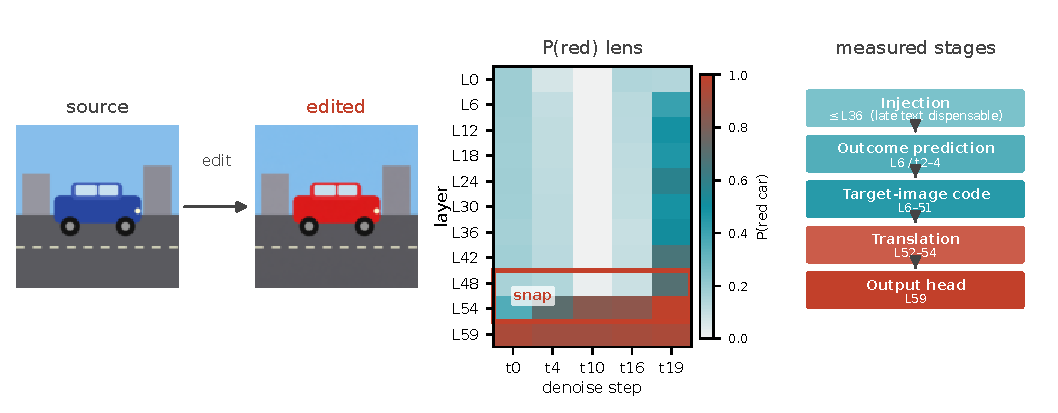
\includegraphics[width=0.98\textwidth]{figs/fig1_teaser/fig1_teaser.pdf}
  \caption{\textbf{Predictable early, translated late.} \textbf{A}: source
  and realized edit. \textbf{B}: frozen-head $P(\text{red car})$ across
  layer and denoising step; a generation-level probe reads the realized
  outcome at L6, whereas the L52--54 translation band makes it readable
  to the frozen output head. \textbf{C}: the five measured stages and
  their layer--time locations. Predictability and frozen-head readability
  are distinct.}
  \label{fig:teaser}
\end{figure*}

\section{Introduction}\label{sec:intro}

Between reading ``turn the car red'' and painting it, what does an image
editor represent? We measure this question across layer and denoising
time. In Qwen, the realized edit is predictable from early hidden states
under a fixed underspecified prompt, yet the frozen output head does not
read the target correctly until a narrow late band translates an
image-like internal code into the velocity convention used by the
sampler. Predictability, frozen-head readability, transplantability, and
writability are therefore measured separately rather than collapsed into
a claim that the output is irreversibly fixed at an early layer.

Watching this happen requires an instrument that did not exist. The
logit lens~\citep{nostalgebraist2020logitlens} and its learned
successor, the tuned lens~\citep{belrose2023tuned}, let us watch a
language model's next-token prediction take shape layer by layer:
project each intermediate residual stream through the model's own final
unembedding and read off a distribution over the vocabulary. Diffusion
transformers (DiTs) that edit
images~\citep{peebles2023dit,qwen2025image} have no analogous tool.
There is no vocabulary for an image patch's hidden state to project
onto, so "what is this layer currently drawing" has, to date, only been
answerable by running the whole model to the end and looking at the
output.

We ask three concrete questions. \textbf{When} does a semantic readout
reach its final value along the 20-step trajectory? \textbf{Where} in the
60-block depth can a frozen head, a fitted probe, or a tuned lens read the
eventual edit? \textbf{What can intervention establish?} We use
transplant to test sufficiency and steering to test writable content.
Whole-token ablation is retained only as a coarse stress test because it
can drive the edited region off-manifold.

Naively porting the logit-lens recipe -- decode every intermediate layer
through the frozen final head and read off a semantic score -- turns out
to be necessary but not sufficient. It reproduces the standard mid-layer
"nothing happens yet" appearance familiar from LLM logit lenses, but a
closer look shows this is itself misleading: a linear probe trained on
the very same activations the frozen head cannot decode reaches near-perfect
cross-seed accuracy 40+ layers earlier. The frozen head is reading the
network's \emph{output-space} code. A generation-level fixed-prompt probe
then shows that the seed-conditioned outcome is predictable in another
basis before the final blocks translate it. Transplant asks a narrower
causal question: whether a donor representation is sufficient to install
that edit in a recipient.

The finding places this work in the ``thinking with
images'' agenda~\citep{su2025thinkingsurvey}, but at the mechanistic
rather than the interface level. That line of work improves multimodal
reasoning by handing a model \emph{explicit} intermediate images to
think with -- sketches, renders, visualization
traces~\citep{hu2024sketchpad,menon2024whiteboard,wu2024vot,li2025mvot,openai2025thinking}.
We find an intermediate target image represented \emph{latently} inside
a generative editor, readable with a layer-specific change of basis,
steerable, transplantable across runs, and translated into the sampler's
velocity convention only near the top. The lens also
exposes this thought mid-struggle: genuinely novel structure starts
late and grows in place while everything else prints immediately, and a
direction pushed without a spatial carrier recruits surrounding tokens
into the object instead of recoloring it. A DiT editor, on this view,
is not merely a tool a multimodal reasoner calls; it natively thinks
with an image before it makes one, and that thought can be watched and
manipulated mid-flight.

\paragraph{Contributions.} \textbf{(1) An instrument, with a discipline.} The first
training-free, frozen-head layer--time lens for a DiT image editor --
including an honest treatment of why the raw, non-rescaled frozen head
is the correct readout despite $>$$10\times$ activation-norm growth
with depth. It is paired with linear probes and three intervention
primitives (ablate, transplant, steer) whose write semantics are stated
exactly, all governed by a falsification-first protocol: pre-registered
predictions, per-image visual verdicts, and standing bit-exactness
gates (\S\ref{sec:method}, \S\ref{sec:protocol}). \textbf{(2) A
mechanism: the editor carries an internal target image.} Under fixed
underspecified prompts, the realized outcome is predictable early across
synthetic and natural images and one independent architecture. In Qwen,
the code is translated into
the velocity code only in a sharp, timestep-invariant band (L52--54)
that is consistent across the tested edit families and survives a
fine-tune and 4-step distillation. A per-(layer, timestep) tuned lens
renders that target-image code directly into a coherent scene at every
depth, confirming there is no hard readability boundary -- only a
change of basis -- and mechanizing the mid-stack's complementary-color
``anti-image'' as the same code read through the wrong one
(\S\ref{sec:tunedlens}). What one direction in that code can
carry obeys a \emph{carrier law}: attributes are writable wherever a
spatial mask supplies the ``where to stop''; object identity yields
not to its probe direction -- read and write subspaces differ -- but to
a graded rank ladder: category at rank 1, coherent instance by rank 4,
material by 16, donor-faithful by rank 64 ($2\%$ of the model
dimension). Transplant establishes sufficiency; steering and the rank
ladder show carrier-bounded writability
(\S\ref{sec:mechanism}--\S\ref{sec:recompose}). \textbf{(3) Validation and levers.}
Held-out early best-of-five selection validates the readout on two architectures with
about 68\% measured compute reduction. Probe direction $+$ silhouette mask gives
donor-free, prompt-free in-place attribute editing with a dose dial
(\S\ref{sec:recompose}); truncating CFG after step 2 saves $45\%$ of
forward passes with all four edit families intact, isolating CFG's real
job as scope resolution (\S\ref{sec:cfgfreelunch}); the layer--time
structure survives step distillation at $7.7\times$ speed, licensing
lens-based analysis of fast variants (\S\ref{sec:generalize},
\S\ref{sec:cfgfreelunch}); and probe-derived saliency, step-budget
prediction, and mid-stack rescue of an under-strength edit close the
loop from reading to optimizing (\S\ref{sec:applications}). A
differential form of the tuned lens (edit run minus a matched no-op
run) turns the internal edit plan into a directly measurable and
previewable quantity -- content is present early but the
differential separates into the edit region only gradually, and
because the no-op run is edit-prompt-independent the same lens forecasts
where a candidate edit will land after just 15\% of the denoising
trajectory (\S\ref{sec:difflens}--\S\ref{sec:previewlever}).
Throughout, four of our own initial misreadings -- including a
forced-choice metric that scored a flat color patch as a perfect
recolor -- are retained in the text as data (\S\ref{sec:limits}).

\section{Related Work}\label{sec:related}

\paragraph{Logit lens and successors.} The logit
lens~\citep{nostalgebraist2020logitlens} projects intermediate
transformer residual streams through the final unembedding matrix,
revealing that language-model predictions often stabilize well before
the last layer. The tuned lens~\citep{belrose2023tuned} fits a small
per-layer affine map instead of reusing the frozen head, trading the
logit lens's zero-training honesty for better-calibrated intermediate
predictions. We deliberately stay on the frozen-head side of this
tradeoff (\S\ref{sec:depthlens}): our interest is in what the network's
own head can already read out, not in the best possible projection.
The linear representation hypothesis~\citep{park2024linear} is the
premise that lets a frozen-head lens and a linear probe disagree
informatively -- if human-interpretable directions are linear, a probe
can find one before the network's own head can read it.

\paragraph{Thinking with images.} A growing line of work has multimodal
models reason \emph{with} images rather than only about them: sketching
intermediate diagrams as a visual chain of
thought~\citep{hu2024sketchpad}, rendering thoughts to a whiteboard
before answering~\citep{menon2024whiteboard}, emitting
visualization-of-thought traces during spatial
reasoning~\citep{wu2024vot,li2025mvot}, and production systems that
crop, zoom, and transform images inside the reasoning
loop~\citep{openai2025thinking}; \citet{su2025thinkingsurvey} survey
the area. In all of these the intermediate image is \emph{explicit} --
produced in pixels as a reasoning step at the model's interface. Our
results supply the complementary, mechanistic half of this agenda:
inside a DiT editor the intermediate image exists \emph{latently}, as a
mid-stack target-image code represented before the final output is rendered,
and it can be read (probe), evaluated (lens), and manipulated (steer,
transplant) without ever being rendered. The editor's characteristic
struggles -- delayed onset when structure is genuinely novel
(\S\ref{sec:when}), membership recruitment when a steered attribute
lacks a spatial carrier (\S\ref{sec:recompose}) -- are then visible as
properties of the thought itself, not just of the output.

\paragraph{Diffusion / image-generation interpretability.} The Diffusion
Lens~\citep{toker2024diffusionlens} decodes intermediate layers of a
text-to-image model's \emph{text encoder} into images, asking when
textual concepts become visually legible before the diffusion process
even starts; our lens instead decodes the image-editing DiT's own
denoising stack, mid-generation. Diffusion models are most commonly
studied through their sampling
process~\citep{ho2020ddpm,song2021ddim,rombach2022ldm} rather than their
internal representations; we build on the flow-matching / rectified-flow
formulation~\citep{lipman2023flowmatching,liu2023rectifiedflow} that
\model{} uses, and on classifier-free
guidance~\citep{ho2022cfg} which the true-CFG sampling loop in
\S\ref{sec:prelim} implements as two sequential passes.

ICM~\citep{zaleska2026icm} supplies the key control for separating an
explicit prompt from a realized generative choice: hold the prompt fixed,
vary the seed, and label the final choice post hoc. Probe-Select
\citep{guo2026probeselect} learns from early denoiser activations to predict
final image quality, while ELECT~\citep{kim2025elect} uses zero-shot early
latent background consistency for candidate selection in instruction editing.
We adopt the fixed-prompt outcome protocol and held-out selection structure,
but predict which outcome a fixed underspecified edit realizes, select relative
to a requested outcome rather than overall quality or preservation, and study
how its code changes across depth. ADE-CoT~\citep{qu2026adecot} goes further as
an efficiency method, combining edit-specific intermediate previews, adaptive
budgets, and opportunistic stopping across multiple editors and benchmarks. Our
five-seed selector is not positioned as a competing test-time-scaling system;
it is a held-out behavioral validation that the measured hidden state carries
the realized attribute.

Breaking the Lock-in~\citep{zhu2026lockin} is the closest temporal neighbor:
it finds early cross-seed convergence in text-to-image sampling and modulates
representations to restore diversity. Our fixed-prompt result concerns which
outcome an image-editing DiT realizes, and our additional axis is transformer
depth -- including the late conversion into the velocity basis -- so we do not
interpret early predictability as irreversible lock-in. DreamReader
\citep{sykora2026dreamreader} is the closest tooling neighbor, unifying
representation extraction, patching, steering, and stitching for text-to-image
U-Nets. Our scope is narrower: a frozen-head/tuned layer--time lens for a joint
text--image DiT editor, with held-out outcome prediction and rendered failure
audits rather than a general-purpose editing toolkit.

\paragraph{Causal interpretability and activation patching.} Causal
tracing / ROME~\citep{meng2022rome} localizes factual associations in
language models by patching activations from a clean run into a
corrupted one and measuring the effect on the output, the same basic
move we use for hidden-state transplant in \S\ref{sec:swap}.
\citet{heimersheim2024activation} catalogue the methodological pitfalls
of activation patching (choice of corruption, direction of the patch,
confounded metrics) that motivate our later rejection of whole-token
ablation as a fine-grained necessity test. Transplant is interpreted
only as sufficiency. This boundary is reinforced by recent work showing that
features can be easy to detect yet produce visual artifacts under
off-distribution steering~\citep{pegoraro2026look}, and that activation
patching with multiple mediators does not identify a unique causal pathway
without stronger assumptions~\citep{zhang2026curse}. Activation
addition~\citep{turner2023actadd} steers language-model generations by
adding a hand- or data-derived direction to the residual stream at
inference time without any gradient step; \S\ref{sec:interventions} and
\S\ref{sec:steer} implement a minimal version of this using the
probe direction from \S\ref{sec:mechanism} rather than a
paired-prompt-derived one.

\paragraph{Diffusion-based image editing.} InstructPix2Pix~\citep{brooks2023instructpix2pix}
and Prompt-to-Prompt~\citep{hertz2023prompttoprompt} are the two
dominant recipes for instruction- and attention-based image editing that
a model like \model{} generalizes and productionizes; CLIP's
image--text embedding space~\citep{radford2021clip} is what we use, for
lack of a better zero-shot alternative, to turn a decoded preview image
into a semantic score in \S\ref{sec:readout}. Most lens mechanics are
validated on \model{}~\citep{qwen2025image}; an independent architecture
is used only for the early outcome-prediction and selection checks. Its
transformer backbone follows
the DiT design~\citep{peebles2023dit}.

\section{Anatomy of a DiT Image Editor}\label{sec:prelim}

\model{} is a flow-matching~\citep{lipman2023flowmatching} DiT
(rectified-flow parameterization~\citep{liu2023rectifiedflow}) with 60
joint text--image transformer blocks (\texttt{transformer\_blocks[0..59]}),
each operating on a shared image-stream hidden state of dimension 3072.
At its native $1024\times1024$ output resolution, the VAE-then-patchify
pipeline (scale factor 8, patch size 2) gives a $64\times64$ grid of
4096 target-image tokens.

\paragraph{Token layout.} Every block's image stream is a concatenation
of the noisy \emph{target} tokens (the image being generated) followed
by the \emph{condition} tokens of every source image supplied to the
edit, in the order the images were passed in. Condition tokens are
injected at $t{=}0$ noise level throughout the trajectory (we refer to
this as \texttt{zero\_cond\_t}): the source image is always presented to
the model as a clean image, not renoised to match the current step. This
means every block, at every timestep, has simultaneous access to (a) the
partially-denoised target and (b) an always-clean copy of the source --
a structural fact we rely on directly when we selectively zero only the
condition-token rows in \S\ref{sec:causal}.

\paragraph{True classifier-free guidance.} At every denoising step the
model is run \emph{twice} -- once conditioned on the edit prompt, once
on an empty/negative prompt -- and the two velocity predictions are
combined, $v = v_{\text{uncond}} + w\,(v_{\text{cond}} -
v_{\text{uncond}})$, with guidance scale $w{=}4.0$ throughout this paper
unless stated otherwise. Because this is two full sequential forward
passes rather than one batched pass, every capture and every
intervention described below is applied identically and independently to
both the conditional and unconditional pass, to avoid producing a
CFG-extrapolation artifact instead of a clean readout or a clean
ablation (see \S\ref{sec:interventions}).

\paragraph{From velocity to a clean-image estimate.} The model predicts a
velocity field $v_\theta(x_t, t)$; at any step $t$ with noise level
$\sigma_t$, the model's current best guess at the fully denoised image
is the standard flow-matching estimate
\begin{equation}
  \hat{x}_0 = x_t - \sigma_t\, v_\theta(x_t, t),
\end{equation}
which can be decoded through the VAE to a preview image at every step
without finishing the trajectory. This is the basis of our \emph{time
lens} (\S\ref{sec:timelens}); the analogous move in \emph{depth} --
decoding an intermediate \emph{layer's} hidden state, not just an
intermediate \emph{timestep's} latent -- is the basis of our \emph{depth
lens} (\S\ref{sec:depthlens}).

\section{Method: A Layer--Time Lens and Causal Probes}\label{sec:method}

\begin{figure}[t]
  \centering
  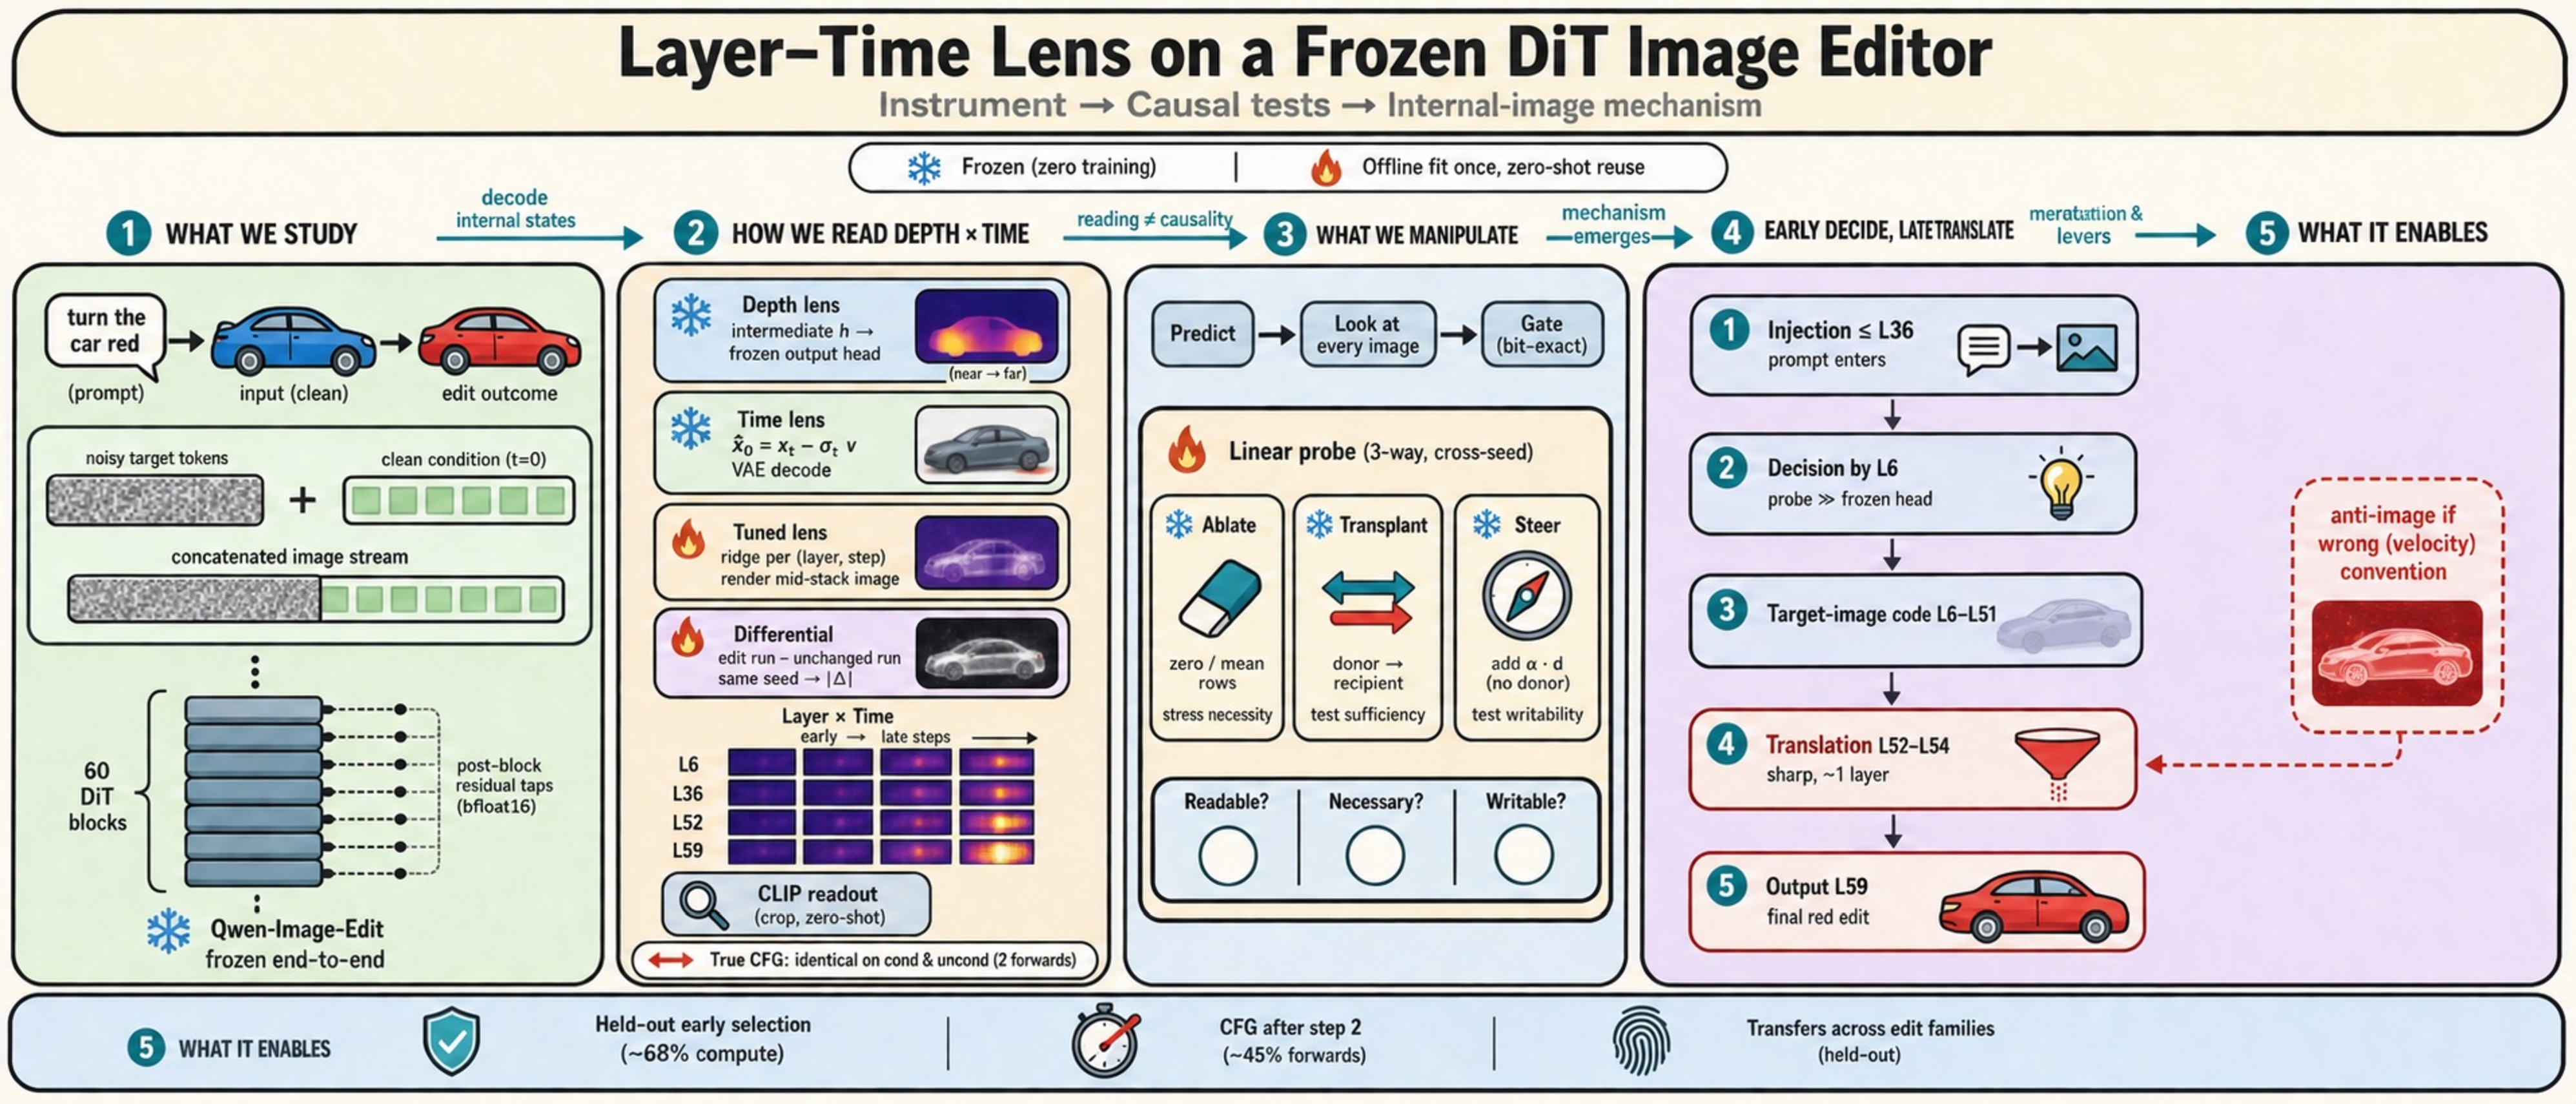
\includegraphics[width=\columnwidth]{figs/fig2_method/fig2_method.pdf}
  \caption{Framework overview (same as main paper Figure~2). Frozen editor,
  four lenses with decode-then-CLIP readout, intervention probes,
  schematic mechanism, and levers; see main text for definitions.}
  \label{fig:method}
\end{figure}

\subsection{Activation capture}\label{sec:capture}
We register a \texttt{register\_forward\_hook} on selected
\texttt{QwenImageTransformerBlock} modules and read the block's own
output tuple \texttt{(encoder\_hidden\_states, image\_hidden\_states)},
i.e.\ capture is on the \emph{post-block residual} -- the same quantity
the next block consumes as input. Capture must use \texttt{bfloat16},
not \texttt{float16}: measured image-stream activations have mean
$|x|\sim10^5$--$10^7$ and an absmax up to $\sim3\times10^{9}$, even at
layer 0, versus fp16's $\pm65504$ range -- casting to fp16 silently
overflows 80--98\% of elements to \texttt{inf}. bf16 is the model's
native compute dtype, so capturing in bf16 is a lossless copy, not a
downcast. Capture is applied independently to the conditional and
unconditional CFG passes and can be restricted to a subset of layers,
timesteps, and image-stream token rows (target vs.\ condition, or a
patch sub-region) to keep storage tractable.

\subsection{Time lens: per-step $\hat{x}_0$ decoding}\label{sec:timelens}
At any denoising step $t$ we decode the flow-matching clean-image
estimate $\hat{x}_0 = x_t - \sigma_t v_\theta(x_t,t)$ (already
introduced in \S\ref{sec:prelim}) through the VAE to get a preview image
of what the model currently believes the final output looks like. This
requires no modification to the model and is cheap (one extra VAE decode
per requested step); it is the axis along which we ask \emph{when} a
semantic readout saturates (\S\ref{sec:when}).

\subsection{Depth lens: the frozen output head}\label{sec:depthlens}
The time lens tells us what the model would output if sampling stopped
at step $t$; we want an analogous readout for stopping at \emph{layer}
$\ell < 59$ within a single step. \model{}'s own final projection from
hidden state to velocity is a fixed, non-trainable
\texttt{AdaLayerNormContinuous} (\texttt{norm\_out}) followed by a linear
\texttt{proj\_out}, both conditioned on the timestep embedding via a
gate that -- we verified by direct weight inspection -- is bit-exact
identical whether it is invoked on the true final layer 59 or is
re-invoked on an intermediate layer's hidden state. We therefore build
the depth lens by feeding an intermediate layer's captured hidden state
through this same frozen head, exactly as if it were the network's
final output, and decoding the resulting pseudo-velocity to a
$\hat{x}_0$ preview via \S\ref{sec:timelens}.

A design choice worth making explicit: \texttt{norm\_out} is a
\emph{non-affine} LayerNorm (no learned scale/shift), so it
per-token-normalizes away the residual stream's norm regardless of what
that norm actually is. Naively "fixing" the depth lens by first
rescaling an intermediate layer's hidden state to the terminal layer's
typical norm is therefore a no-op in principle -- and we confirmed this
empirically three ways: (i) simulating the rescale on the frozen head's
weights directly (relative deviation $2\times10^{-6}$), (ii) running the
full raw and rescaled pipelines end to end and diffing the decoded
images (max pixel difference 11/255, max CLIP-score difference 0.038),
and (iii) visual inspection. We report a formal self-consistency gate
alongside every lens grid we compute (raw vs.\ rescaled variants agree,
\texttt{max\_rel\_diff}$=0$ on the cases we checked). The \emph{raw},
non-rescaled head is therefore the honest lens, and is what we use
throughout; where rescaling would have mattered, it would have meant our
frozen-head assumption itself was wrong, not that rescaling was needed.

\subsection{Semantic readout: decode-then-CLIP}\label{sec:readout}
Neither the time lens nor the depth lens is itself a semantic score --
both produce an image (a full preview or a per-layer pseudo-preview).
To turn a decoded image into a number we crop the relevant region
(a hand-annotated bounding box, or the whole image for global edits) and
score it zero-shot against a small bank of natural-language labels with
CLIP~\citep{radford2021clip} (\eg{} "a red car" vs.\ "a blue car" vs.\ "a
green car"), reporting the softmax probability on the target label.
Two consequences follow directly from this being a \emph{decode-then-
score} readout rather than a probe on the hidden state itself. First, it
is a whole-crop judgment, not a per-token one -- we do not claim
per-patch CLIP scores are meaningful at the $16$px patch pitch of the raw
target grid, hence cropping to a $\gtrsim$224px-equivalent window before
scoring. Second, it inherits every failure mode of zero-shot CLIP on
possibly out-of-distribution decoded previews: we \emph{gate} on decode
coherence (only trust a CLIP score once the decoded preview looks like a
plausible image, not pure noise) and flag every place in
\S\ref{sec:exp}--\S\ref{sec:limits} where this gate is violated (most
consequentially, a very-early-layer, very-early-step decode of
"noise" is mis-scored as "a beach background" at $P{=}0.795$; see
\S\ref{sec:limits}).

\subsection{Interventions: stress tests, transplant, and steering}\label{sec:interventions}
Reading a lens value tells us the network's representation is
\emph{consistent with} a hypothesis, not that the hypothesis is
causally correct. We use two interventions, both implemented as the same
kind of forward hook as capture, but \emph{overwriting} the block's
output before it is returned:

\textbf{Whole-token stress test.} Zero (or mean-replace, using the mean of the
non-ablated target tokens in that same forward call) selected target
rows of the image hidden state at selected layers. Because this is a
post-block \emph{residual overwrite}, it destroys that token position's
entire representation for \emph{every subsequent block} in the same
forward pass -- there is no mechanism for a later block to "see through"
the overwrite. An empty intervention spec is verified to reproduce the
baseline bit-for-bit. A non-empty overwrite is intentionally blunt:
destroying an entire residual token across many layers can move the
edited region off-manifold, so the result diagnoses failure and recovery
rather than the causal role of a specific readable direction.

\textbf{Transplant (cross-run swap).} Overwrite selected target rows of
a "recipient" run's hidden state, at selected layers and timesteps, with
the corresponding rows captured from a different "donor" run (same
seed, same source image, different edit prompt or a stronger sampling
setting), matched by timestep, layer, and patch coordinate. This tests
\emph{sufficiency}: if the donor's representation, spliced in, is enough
to flip the recipient's decoded output toward the donor's edit, the
donor layer band is causally sufficient for that edit. We do not infer
necessity from the separate whole-token stress test.

\textbf{Steer.} Add a fixed direction to selected target rows at
selected layers, scaled by a strength $\alpha$ (in units of the
per-row RMS activation scale), rather than overwriting the rows
outright. We take the direction from the linear probe of
\S\ref{sec:mechanism} -- the difference between the mean captured
hidden state of a "red" run and a "green" run at the probe's own
cell (L12, $t{=}4$), restricted to the car region -- and add
$\alpha\,d_{\text{red}}$ to the recipient's car-region rows at layers
6--23, all steps, on both CFG passes. Unlike transplant, this requires
no donor forward pass at all, only a single stored direction vector.

All interventions are applied identically and independently to the
conditional and unconditional CFG pass at every affected step, for the
reason given in \S\ref{sec:prelim} -- doing otherwise would compare a
lopsided, extrapolated CFG combination against a clean one rather than
isolating the effect of the intervention itself.

\subsection{Protocol: predict, look, gate}\label{sec:protocol}
The machinery above is reproducible in the ordinary sense (fixed seeds,
frozen weights, released code and run artifacts; constants in
Appendix~\ref{app:repro}). This subsection states the part of the
method that makes the \emph{reasoning} reproducible -- three rules
applied to every experiment in the paper. \textbf{Predict, then run.}
Every intervention experiment was pre-registered: the expected outcome
per condition was written down before launching the run, and
refutations are reported as prominently as confirmations -- several of
our headline findings, including the carrier law
(\S\ref{sec:recompose}) and distillation resilience
(\S\ref{sec:cfgfreelunch}), are pre-registered predictions that failed
in an informative direction. \textbf{Look at every image.} Zero-shot
CLIP has four failure modes we document (forced-choice inflation,
texture shortcuts, thumbnail pseudo-motion, and under-scoring genuine
success; \S\ref{sec:limits}), so no intervention verdict rests on CLIP
alone: every run directory carries a per-image visual verdict file,
recorded before the aggregate metrics were read, and where the two
disagree the visual verdict wins. Two of our four self-corrections
originated exactly there -- and one ran the other way (eyeballed
thumbnails misled us until quantification at native resolution caught
it; \S\ref{sec:limits}), which is why the rule is ``both, recorded
separately,'' not ``eyes over numbers.'' \textbf{Gate the instrument.}
An empty intervention spec must reproduce the baseline bit-for-bit,
and the frozen head must pass its raw-vs-rescaled self-consistency
check (\S\ref{sec:depthlens}) on every lens grid; both are standing
regression checks re-run per experiment, not one-time validations.
Porting the whole method to another DiT editor therefore needs only
(a) a post-block residual hook in the model's native dtype
(\S\ref{sec:capture}), (b) the frozen-head gate to license the depth
 lens, and (c) region-restricted 3-class probes to obtain semantic
directions; the cross-model replication in \S\ref{sec:generalize} is
this recipe executed unchanged on two further checkpoints.

\section{Experiments}\label{sec:exp}
All experiments use \model{}, true CFG scale 4.0, 20 inference steps,
seed 0 unless stated otherwise (\eg{} the cross-seed probe in
\S\ref{sec:mechanism} additionally uses seed 1). Two running examples
recur throughout: \emph{car\_red} ("turn the car red" on a synthetic
flat-vector car scene) and \emph{beach\_background} ("change the
background to a beach" on a real photo), chosen because they represent
opposite ends of the "how much does the source image constrain the
edit" spectrum -- a local, preserving color edit vs.\ a global,
non-preserving background replacement. Later generation-level studies
use 48 independent seeds per training set and 12 held-out five-seed
groups per selector. The subsections separate early outcome
predictability, late code translation, transplant sufficiency,
carrier-bounded writability, and practical levers.

\subsection{When: semantic saturation is edit-dependent}\label{sec:when}

\begin{figure}[t]
  \centering
  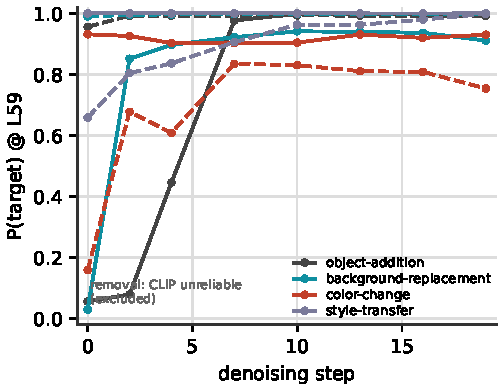
\includegraphics[width=\columnwidth]{figs/fig3_commit_curves/fig3_commit_curves.pdf}
  \caption{Time-lens $P(\text{target})$ at the final readable layer
  (L59) across the denoising trajectory, for 8 of our 10 battery cases
  (\S\ref{sec:when}), colored by edit category. Preserving edits
  (color-change, most background-replacement) print near their final
  value from step 0; \emph{add\_boat}, the one novel-object insertion,
  only rises after step $\sim$4. Object-removal cases (2 of 10) are
  excluded here and shown separately in Table~\ref{tab:battery}: their
  target label ("an empty desk with no cup") is not a CLIP-friendly
  category and the readout is flat/noisy regardless of the true edit
  outcome (\S\ref{sec:limits}).}
  \label{fig:commit}
\end{figure}

The gradual-development picture makes its first testable claim in
time: if the semantic readout surfaced progressively, its saturation
step should be late and roughly uniform across edits. It is neither.
Running the time lens (\S\ref{sec:timelens}) over a battery of 10 cases
spanning 5 edit categories (color-change, background-replacement,
object-addition, object-removal, style-transfer; 2 cases each) shows the
saturation step is not fixed across the tested edits. Table~\ref{tab:battery} reports, for
each case, the step at which the time-lens $P(\text{target})$ first
reaches within 0.05 of its step-19 value (the legacy run key is
\texttt{commit\_step}) and the
first depth-lens layer at which the same threshold is first crossed at
step 0 (\texttt{first\_layer}).

\begin{table}[t]
\centering
\small
\begin{tabular}{lccc}
\toprule
case & category & saturation & first \\
 & & step & layer \\
\midrule
color\_car        & color         & 0 & 54 \\
color\_cup        & color         & 2 & 54 \\
bg\_forest        & background    & 0 & 12 \\
bg\_beach         & background    & 2 & 0  \\
style\_sketch     & style         & 0 & 36 \\
style\_watercolor & style         & 2 & 0  \\
add\_latte        & addition      & 0 & 0  \\
add\_boat         & addition      & 7 & 54 \\
remove\_cup$^\dagger$      & removal & 0 & 0 \\
remove\_laptop$^\dagger$   & removal & 0 & 0 \\
\bottomrule
\end{tabular}
\caption{Semantic saturation step and earliest head-readable layer, all 10 battery
cases (data: \texttt{runs/a5\_aggregate.json}). $^\dagger$Object-removal
CLIP readouts are unreliable (\S\ref{sec:limits}); the saturation/first-layer
values shown for these two are not meaningful and are listed only for
completeness.}
\label{tab:battery}
\end{table}

At the resolution of Table~\ref{tab:battery} -- a coarse, three-value
CLIP-threshold discretization (steps 0, 2, or 7) -- it is tempting to read
a graded \emph{layout-novelty} gradient into these numbers: color and
texture edits saturate at step 0, edits that introduce a new region of
content one or two steps later, and the one wholesale new-object
insertion (add\_boat) latest of all. A follow-up study puts this reading
to a direct, quantitative test rather than leaving it as a plausible
narrative. We re-ran the finer, IoU-mask-based onset measurement of
\S\ref{sec:limits}/Appendix~\ref{app:repro} (there applied only to
add\_boat) on ten further cases spanning the same five categories (20
cases total; \texttt{runs/g5\_onset\_law}) and asked whether either final
edit area or an edge-based layout-novelty proxy predicts onset step
continuously. Neither does: Spearman $\rho=0.244$ ($p=0.300$) for the
novelty proxy and $\rho=-0.436$ ($p=0.055$) for area -- the area
correlation, such as it is, runs in the \emph{wrong} direction to explain
a delay, driven entirely by the two slowest cases having unusually
\emph{small}, not large, final edit regions. Eighteen of the twenty cases
-- spanning final-edit-area fraction $0.003$ to $0.99$ -- onset at step 0
regardless of how large, novel-looking, or global the finished edit is.
Only two cases delay: add\_boat (onset step 4) and \emph{add\_runner}, a
second wholesale insertion of a person with no partial figure to extend
(onset step 2); edits that add detail \emph{onto} an already-present
object -- latte art onto an existing cup, a ladybug onto an existing pine
cone -- onset at step 0 like every other case. The honest finding is
therefore categorical, not continuous: onset is delayed only when an edit
inserts a genuinely novel structure with no existing pixels to build on,
and we explicitly do not claim a continuous novelty law beyond that
(\texttt{runs/g5\_onset\_law}, Appendix~\ref{app:repro}). This categorical
split is unaffected by the softening above: in Table~\ref{tab:battery},
the same edits whose readout saturates late in time also require the deepest
first-readable layer.
\subsection{Where in depth: late materialization, inverted mid-stack}\label{sec:depth}

\begin{figure}[t]
  \centering
  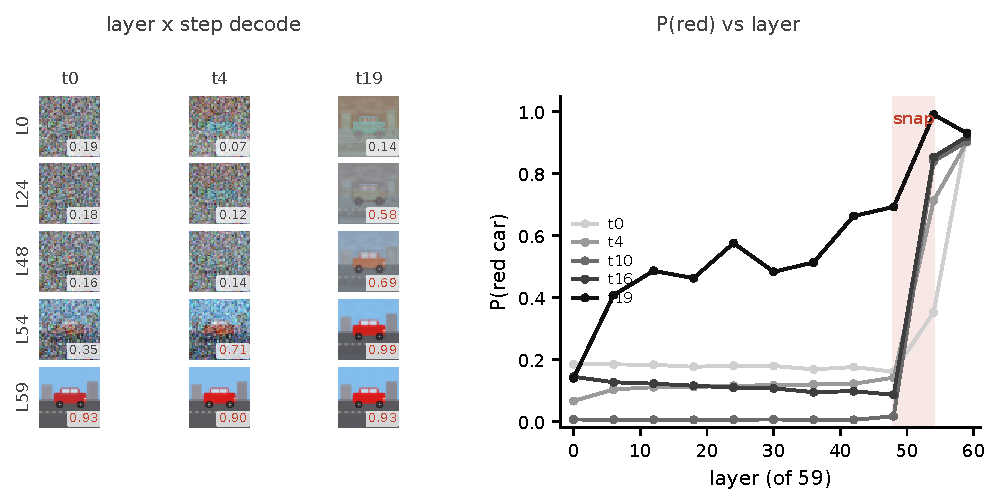
\includegraphics[width=\columnwidth]{figs/fig4_depth/fig4_depth.pdf}
  \caption{Depth lens on \emph{car\_red}. Left: decoded depth-lens
  preview at 5 layers $\times$ 3 steps, with the frozen head's
  $P(\text{red car})$ overlaid (red text $>0.5$); L0--L48 renders a
  \emph{blue/tan car} (source color or its complement), not red, despite
  the final output being red. Right: $P(\text{red car})$ vs.\ layer for
  5 timesteps -- flat and low through L42, then a sharp rise
  ("snap", shaded) between L48 and L54 that lands within a few points of
  the L59 value.}
  \label{fig:depth}
\end{figure}

Fixing the timestep and instead sweeping the depth lens (\S\ref{sec:depthlens})
across layers reveals a second, orthogonal emergence axis. For
\emph{car\_red}, Figure~\ref{fig:depth} shows $P(\text{red car})$ is flat
and \emph{low} (0.06--0.18) from layer 0 through layer 42, at every
timestep we tried -- not because the depth lens has nothing to read
(the decoded previews at these layers are coherent, recognizable car
scenes, just the wrong color), but because the frozen head, at this
depth, reads out a color \emph{other than} the eventual output. At
several layer/step combinations the highest-scoring label is "a blue
car" or "a green car" rather than "a red car" (\eg{} at L0, step 10,
$P(\text{blue})=0.98$ vs.\ $P(\text{red})=0.007$; full grid in
\texttt{runs/a1\_car\_red/lens\_grid.json}). Then, between layers 48 and
54, $P(\text{red car})$ snaps upward at every timestep we measured (\eg{}
at $t{=}4$: $0.14\to0.71$; at $t{=}16$: $0.10\to0.85$), landing within a
few points of the terminal L59 value by L54 and matching it by L59. The
same qualitative pattern -- flat-then-snap in the last $\sim$10 layers --
holds for \emph{beach\_background}, with one notable wrinkle we treat as
a caveat rather than a finding: at L54, $t{=}0$, the decoded preview is
still almost pure sampling noise, yet CLIP scores it $P(\text{beach})=0.795$,
higher than the correctly-gated, genuinely-coherent L59 reading at the
same step ($0.029$, because L59 at $t{=}0$ correctly still shows the
original fence background). We do not treat the L54/$t$0 number as
evidence of anything about the model; it is exactly the decode-coherence
failure mode flagged in \S\ref{sec:readout} and revisited in
\S\ref{sec:limits}.

This late, sharp depth transition inverts a natural expectation. If the
mid-stack literally "had no opinion yet" about the edit, layer-band
ablation should hurt uniformly little in the mid-stack and matter only
near the readable layers. \S\ref{sec:causal} shows this is false for
\emph{car\_red}: the causally load-bearing layers are the \emph{early}
ones, well before the depth lens can read anything out of them at all.
The depth lens's blind spot is not the same thing as the network's.
\subsection{Mechanism: two codes}\label{sec:mechanism}

\begin{figure*}[t]
  \centering
  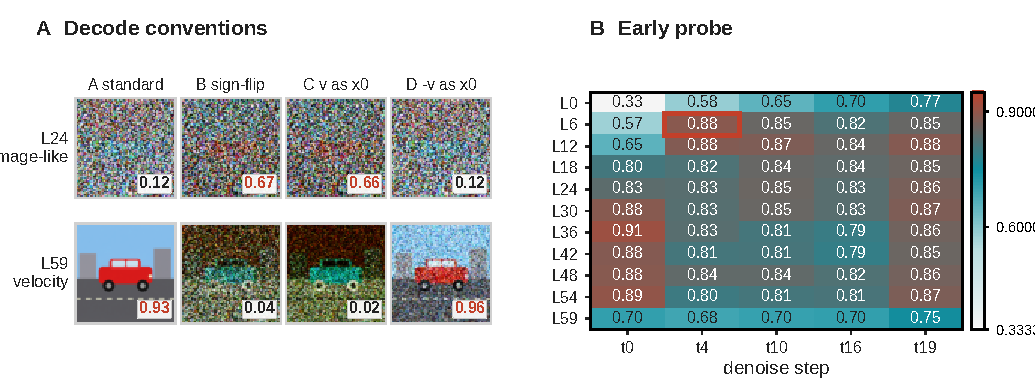
\includegraphics[width=0.93\textwidth]{figs/fig5_mechanism/fig5_mechanism.pdf}
  \caption{\textbf{A}: four ways of turning an intermediate layer's frozen-head
  output into an image for \emph{car\_red} at $t{=}4$ (A: standard
  $\hat{x}_0{=}x_t{-}\sigma_t v_\ell$; B: sign-flipped
  $x_t{+}\sigma_t v_\ell$; C: $v_\ell$ decoded directly; D: $-v_\ell$
  decoded directly). At L24 the standard decode (A) is wrong-colored
  while the sign-flipped/direct-$v$ decodes (B, C) already look red; at
  L59 this reverses. \textbf{B}: cross-seed 3-way probe accuracy (chance
  $=0.33$) by layer/step; the headline cell L6/$t$4 (red outline,
  $0.883$) is far above the frozen-head reading at the same cell
  (\S\ref{sec:depth}), and probe accuracy \emph{drops} at L59 relative
  to L48--L54.}
  \label{fig:mechanism}
\end{figure*}

Here we separate early predictability from late frozen-head readability.
The depth-lens snap in
\S\ref{sec:depth} is consistent with two very
different underlying stories: either the target-image content simply
does not exist yet in the mid-stack representation, or it exists but is
represented in a form the frozen head -- built to consume the network's
\emph{final}-layer convention -- cannot correctly parse. We distinguish
these with two further probes.

\textbf{Four-variant decoding.} At an intermediate layer $\ell$, the
frozen head produces a 64-channel per-token vector $v_\ell$ that we
normally treat as a velocity and combine with the current noisy latent
as $\hat{x}_0 = x_t - \sigma_t v_\ell$ (variant A, our standard depth
lens). We additionally decode: (B) the sign-flipped combination
$x_t + \sigma_t v_\ell$; (C) $v_\ell$ itself, decoded directly as if it
already were a clean latent; and (D) $-v_\ell$ decoded directly. For
\emph{car\_red} at $t{=}4$, at L24 the standard decode (A) scores
$P(\text{red car}){=}0.12$ -- still the wrong color -- while the
sign-flipped and direct-$v$ decodes (B, C) already score $0.67$ and
$0.66$. At L59, this \emph{reverses}: A scores $0.93$ (correct) while B
and C collapse to $0.04$ and $0.02$. D tracks A closely at every layer
(both low mid-stack, both high at L59). This crossover is a controlled,
four-way confirmation that the mid-stack representation is not simply
"blank" -- it already encodes something that decodes as approximately
the right content under the \emph{opposite} sign convention -- and that
whatever reconciles the two conventions happens in the same narrow band
(L48--L54) where the standard depth lens snaps.

We do not, however, read this as a literal single-axis sign inversion.
A per-channel regression of each intermediate $v_\ell$ against the final
$v_{59}$ shows the fraction of the 64 channels with a \emph{negative}
slope is essentially zero at every layer/step cell we checked
(mean $0.003$, max $0.0625$ across our grid) -- almost no individual
channel literally flips sign. Yet the aggregate cosine similarity
between $v_\ell$ and $v_{59}$ can be as low as $0.33$ (L0, $t{=}16$)
before rising to $\ge 0.86$ only inside the last $\sim$6 blocks. The two
measurements together say the mid-stack-to-final transition is better
described as a \emph{whole-vector re-weighting across channels} than as
a bit-flip on a single "color sign" axis; "sign flip" in variant B is a
useful coarse diagnostic (which global combination formula decodes
better), not a mechanistic claim about one direction in activation
space.

\textbf{Explicit-prompt basis diagnostic.} A frozen head is one specific,
non-trainable projection; a fitted linear probe asks whether a variable is
linearly present in some other basis. We first fit a 3-way probe predicting
which of three colors was explicitly requested, training on one seed and
testing on another over an $11\times5$ layer--step grid
(Figure~\ref{fig:mechanism}, right; chance $=0.333$). At L6, $t{=}4$ its
accuracy is $0.883$, while the frozen-head lens at the same cell reads
$P(\text{red car})=0.111$. This establishes a basis mismatch, but because
the color word differs across prompts it does \emph{not} by itself show
that a seed-conditioned realized outcome is predictable. The terminal L59
probe is lower than L48--L54 ($0.70$--$0.75$ vs.\ $0.80$--$0.89$), a
color-specific loss of linear separability after the translation.

\textbf{Fixed-prompt generation-level outcome probes.} To remove the
instruction-label confound, we hold both source and prompt fixed
(``change the car to a different color''), vary only the seed, and label
each final image post hoc. Each generation contributes one mean-pooled
vector. On 48 new seeds, the L6/$t$4 probe reaches 0.667 balanced accuracy
against 0.333 chance (500-permutation $p=0.002$); a circular decoder at
L6/$t$2 reduces final-hue MAE from $22.3^\circ$ to $8.3^\circ$
($R^2=0.815$). A pre-registered real-photo follow-up preserves one
continuous mug replication ($17.0^\circ\to10.7^\circ$, $p=0.005$) and one
eye null ($p=0.796$); a separate natural-photo tree replication gives
$55.9^\circ\to11.4^\circ$ ($p=0.005$). On the independent 40-block Boogu
editor, L4/$t$2 gives $39.9^\circ\to6.9^\circ$ ($p=0.005$), though its
terminal layer is stronger rather than weaker.

\textbf{Held-out early selection.} The probes also support a practical
test on unseen seeds. On Boogu, an L4/$t$2 selector chooses a successful
recolor in 8/12 new five-seed groups versus 20\% random expectation
($p=4.1\times10^{-5}$); the L4/$t$0 control is null ($p=0.188$). On 12
Qwen, two separately pre-registered target tasks pass. On 12 tree groups,
an L6/$t$2 selector reduces mean target error from $95.2^\circ$ under
random selection to $46.5^\circ$ (oracle $43.2^\circ$), with mean rank
1.17 and exact $p=3.7\times10^{-7}$; L6/$t$0 is null ($p=0.381$). A
current-environment car replication reduces $25.7^\circ$ to $11.1^\circ$
(oracle $8.7^\circ$), with mean rank 2.00 and $p=0.0086$. Its L6/$t$0
control retains partial signal (mean rank 2.17, $p=0.0256$) but misses the
frozen rank and $p$ gates. All selection runs use actual interrupted
captures and winner reruns, reducing measured best-of-five compute by
about 68\%. This is closest-candidate selection: some groups contain no
candidate near the requested target hue.

\begin{figure*}[t]
  \centering
  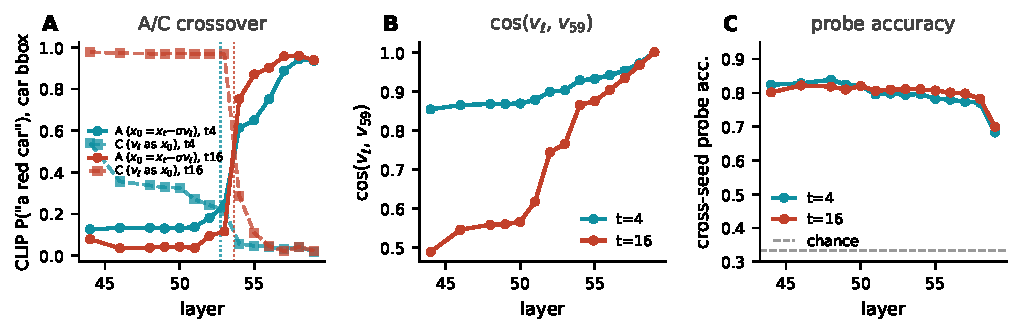
\includegraphics[width=0.98\textwidth]{figs/fig10_boundary/fig10_boundary.pdf}
  \caption{A dense, every-layer sweep of \emph{car\_red} over L44--L59
  sharpens the coarse L48/L54 snap of Figure~\ref{fig:depth} to a precise
  boundary. \textbf{A}: the standard decode (A) and the direct-$v$ decode
  (C) cross between L52 and L54 at both steps shown. \textbf{B}: cosine
  similarity of the intermediate pseudo-velocity to the terminal $v_{59}$
  rises sharply in the same band. \textbf{C}: cross-seed probe accuracy is
  flat from L44 through L58 and drops only at the terminal layer.}
  \label{fig:boundary}
\end{figure*}

\textbf{A dense boundary sweep confirms the transition is sharp and
timestep-invariant.} The four-variant crossover and the L59 probe dip
above were both measured on the coarse, $\sim$6-layer grid used
throughout this paper. To ask how narrow the translation actually is, we
re-ran the A/C crossover, the cosine-to-$v_{59}$ trace, and the cross-seed
probe at \emph{every} layer from L44 to L59, at $t{=}4$ and $t{=}16$
(Figure~\ref{fig:boundary}). The crossover is sharp: at $t{=}16$ the
transition width -- the gap between the last layer where the direct-$v$
decode still clearly wins and the first layer where the standard decode
does -- is a single layer, with the crossover midpoint at L53.6; at
$t{=}4$ the same midpoint is L52.7 with a wider, 4-layer transition band.
The two midpoints differ by under one layer ($0.93$), so the boundary's
\emph{location} is essentially timestep-invariant even though its
sharpness is not. The cross-seed probe grid resolves a second, and we
think more important, point: probe accuracy is not merely "higher at
L48--L54 than at L59" as the coarse grid suggested -- at this density it
is close to \emph{flat}, sitting in a $0.77$--$0.84$ band across every
sampled layer from L44 through L58 at both steps, and drops only at the
terminal layer L59 ($0.68$--$0.70$). In other words, the sharp translation
in panels A/B (which changes what the frozen head can read) does
\emph{not} coincide with any loss of linear separability until the very
last block -- the target-image code's linear decodability survives the
translation intact through L58 and is degraded only by the final,
velocity-specific projection. Translation and separability collapse are
therefore two distinct events sharing a neighborhood, not one event: the
former happens across L52--54, the latter only at L59.

\subsection{Rendering the internal image: a tuned lens}\label{sec:tunedlens}

\begin{figure*}[t]
  \centering
  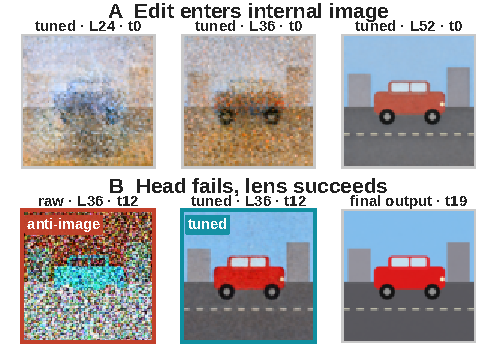
\includegraphics[width=0.52\textwidth]{figs/fig12_tuned_lens/fig12_tuned_lens.pdf}
  \caption{A tuned lens renders the internal image the frozen head
  cannot read. \textbf{A}: per-(layer, timestep) ridge translators, fit on
  \emph{remove}/\emph{background}/\emph{addition} edits and evaluated
  zero-shot on the held-out \emph{car\_red} color edit, decode a
  coherent scene at every depth at $t{=}0$ -- pixels here are pure
  noise, so every pixel of the decode comes from the velocity code
  alone. The source's blue car (L12--L24) turns orange-red (L36), the
  scene composes fully (L44), and the car is fully red by L52: the
  edit entering the internal image, watched layer by layer. \textbf{B}: at
  $t{=}12$ the raw frozen head (\S\ref{sec:depthlens}) renders the
  identical L36 hidden state as a color-inverted ghost -- a cyan car
  under a red-brown sky, the complement of the true scene -- while the
  tuned lens at the same cell is already coherent; the model's actual
  final output is shown for reference.}
  \label{fig:tunedlens}
\end{figure*}

\S\ref{sec:mechanism} showed the mid-stack target-image code is
linearly readable in \emph{some} basis, using a probe built for one
narrow purpose (three-way color classification). Elsewhere in this
paper we deliberately stay on the frozen-head side of the
logit-lens~\citep{nostalgebraist2020logitlens}/tuned-lens tradeoff
(\S\ref{sec:related}), because our
interest is in what the network's own head can already read. Here we
cross to the other side for one narrow diagnostic purpose -- can the
mid-stack code be decoded back into an actual \emph{image}, at every
depth, rather than just a probe score? We fit a tuned
lens~\citep{belrose2023tuned}: a per-(layer, timestep) ridge
regression from the hidden state $h_\ell$ (3072-d) to the
conditional-pass velocity (64-d), one dictionary per cell, trained
only on \emph{remove}, \emph{background}, and \emph{addition} edits
with $\lambda$ chosen on a held-out 10\% split of training tokens,
then evaluated zero-shot on \emph{car\_red}, an edit family it never
saw during fitting. Held-out $R^2$ at L59 reaches $0.998$; a separate,
standing identity check on the same run confirms this is measured
against a verified-correct target, not a pipeline artifact --
decoding the L59 hidden state through the model's own frozen head
reproduces the model's actual velocity bit-for-bit
(max$|$diff$|=0$ at every step), the same raw-head self-consistency
gate used throughout this paper (\S\ref{sec:depthlens}).

\textbf{No hard affine readability boundary exists.} A pre-registered
prediction that tuned-lens readability would itself have a boundary,
between the shallow layer where a probe first predicts the outcome and
the L52 layer where the frozen head does, is refuted -- in the
interesting direction. Every depth we tried, down to L6, decodes a
coherent scene once given its own per-(layer, timestep) dictionary, and
held-out $R^2$ rises with depth (L6: $0.73$--$0.89$
across steps, to L59: $0.998$), with a per-step translator beating a
single pooled-over-$t$ one everywhere -- confirming the velocity code
is time-dependent, not just depth-dependent. The L52--54 boundary of
\S\ref{sec:depth}--\S\ref{sec:mechanism} is a property of the
\emph{frozen} head's one fixed projection, not of the representation
itself: give any layer the right per-cell change of basis and it is
legible.

\textbf{The edit enters the internal image at the first step,
watchably, layer by layer.} At $t{=}0$ the pixels are still pure
noise, so $\hat x_0$ is determined entirely by the decoded velocity --
nothing here is contaminated by an already-informative latent.
Figure~\ref{fig:tunedlens} (top) shows the source's blue car persisting
through L24, turning orange-red by L36, the whole scene composing by
L44, and the car fully red by L52. This renders how target-image content
changes through depth rather than inferring an irreversible transition
from a probe score.

\textbf{The anti-image, mechanized.} The mid-stack frozen-head decode
does not merely fail to show red (\S\ref{sec:depth}); at $t{\ge}8$ it
renders a color-\emph{inverted} ghost of the L36 hidden state -- a
cyan car under a red-brown sky, against a true scene of a red car
under blue sky (Figure~\ref{fig:tunedlens}, bottom). The tuned lens
explains why: the mid-stack code is image-like, and $\hat x_0 = x_t -
\sigma v$ flips the sign of an image-like quantity when it is forced
through a head built to consume a velocity-like one.

\textbf{The translator is a model property, not an edit property.}
Trained with zero color edits, it renders the held-out color edit
perfectly at every depth: the goal-to-flow translation the L52--54
band performs late is, for readout purposes, close to a
per-(layer, timestep) affine change of basis that holds across edit
families, not a fact about \emph{car\_red} specifically.

\textbf{Family generality, and the time axis.} The identical frozen
per-(layer, timestep) dictionaries above -- fit once on
\emph{remove}/\emph{background}/\emph{addition} and already evaluated
zero-shot on \emph{car\_red} -- transfer with \emph{zero further
retraining} to six more held-out cases spanning style, two further
color edits, removal, background, and addition
(\texttt{runs/k1b\_transfer\_battery}): every one decodes a coherent
internal image at every depth we tried. Held-out $R^2$ follows the
same depth trend as \emph{car\_red} across all six cases -- low points
$0.65$--$0.84$ at L12/L24, $t{=}0$, rising to $0.978$--$0.994$ by L52.
The decisive case is \emph{add\_runner} (Figure~\ref{fig:k1btransfer}):
at L52, $t{=}0$ -- the same depth and step at which \emph{car\_red}'s
final color was already visible -- the internal image shows an
empty path, no runner; a blurred figure appears mid-path by $t{=}2$;
a clear blue-shirted runner is rendered by $t{=}4$. The already-known
invention-class delayed onset (\S\ref{sec:when}) is here watched
directly on the internal image's own time axis, with the depth
assembly band unchanged -- both axes of ``watching the model think''
rendered at once. \emph{style\_ink}, a stylization family neither the
translator's training set nor the \emph{car\_red} test case saw, is
already ink-styled by mid-depth.

\begin{figure}[t]
  \centering
  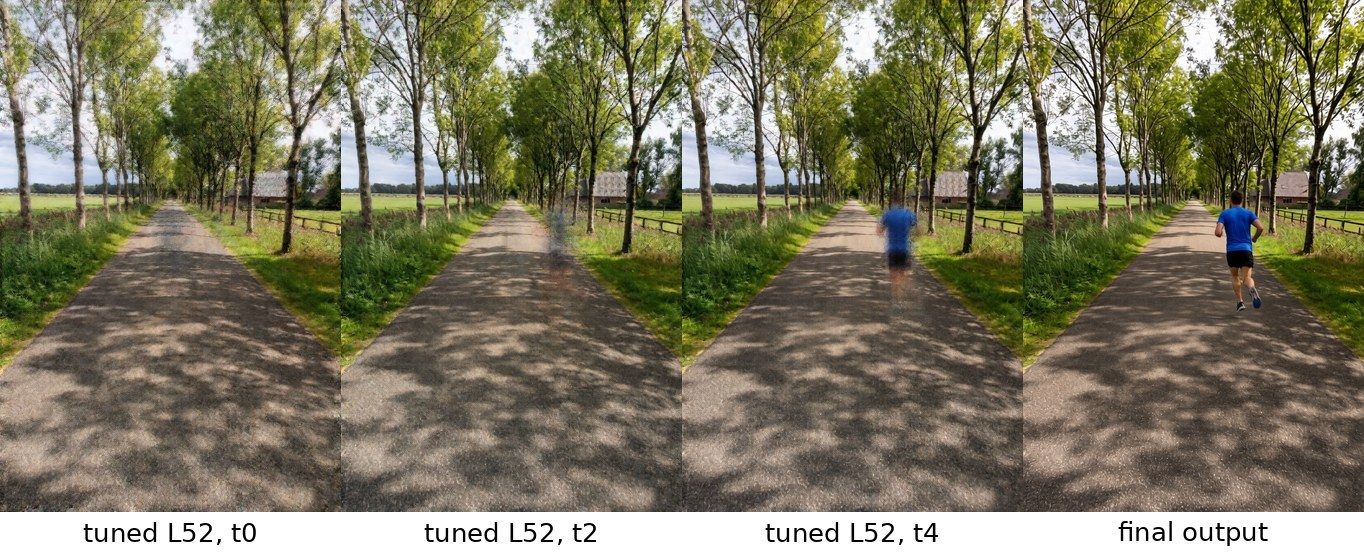
\includegraphics[width=\columnwidth]{figs/fig13_transfer_onset/fig13_transfer_onset.jpg}
  \caption{Zero-retrain transfer to a held-out \emph{add\_runner} edit
  (\S\ref{sec:tunedlens}), decoded at L52 through the same translators
  fit for Figure~\ref{fig:tunedlens}. At $t{=}0$ the internal image
  shows an empty path; a blurred figure appears by $t{=}2$; a clear
  blue-shirted runner is rendered by $t{=}4$ -- the invention-class
  delayed onset of \S\ref{sec:when}, watched directly on the internal
  image's time axis rather than inferred from a probe score. Final
  output shown for reference.}
  \label{fig:k1btransfer}
\end{figure}

\textbf{Caveats.} $t{\ge}12$ columns have small $\sigma$ ($\hat x_0
\approx$ the latent regardless of $v$) and are excluded from the
depth-sweep and $R^2$ claims above, which rest on $t{=}0$--$4$. The
anti-image is a separate observation at $t{\ge}8$, not a quantity
read off those excluded columns, and is not subject to that
exclusion: raw mid-stack previews
\emph{anti}-correlate with the final image (pixel Pearson
$r\approx-0.40$ at L24--L44, $t{=}12$) while the tuned decode of the
same L36 state reaches $r=+0.99$. Held-out $R^2$ is dominated by easy
reconstruction variance rather than edit-region-specific signal;
\S\ref{sec:difflens} closes this gap with a differential form of the
same lens that isolates the edit-specific signal directly.

\subsection{Differential lens: content is early, separation is
gradual}\label{sec:difflens}

\S\ref{sec:tunedlens}'s held-out $R^2$ conflates two things: how well
the frozen per-(layer, timestep) dictionaries reconstruct \emph{any}
scene, and how much of that fidelity is specific to the edit itself.
Isolating the second requires a control. We run the identical source
image and seed through the tuned-lens capture twice -- once with the
edit prompt, once with the literal instruction ``keep the image
unchanged'' -- and decode both runs through the same frozen
dictionaries fit in \S\ref{sec:tunedlens} (\emph{no refitting}).
Because the two runs share a seed, their $t{=}0$ latents are
bit-identical, so at the very first step any difference between the
two decodes comes entirely from the two prompts' differing velocity
predictions: $D_{\ell,t} = |\text{decode}(h_\ell^{\text{edit}}) -
\text{decode}(h_\ell^{\text{unchanged}})|$ isolates the internal edit
plan, with the reconstruction component of the tuned-lens decode
canceling out by construction (up to later-step collateral trajectory
divergence between the two runs, discussed below). We report three
statistics of $D$ against the ground-truth edit region $R$ (the
top-10\% of the two runs' final-output pixel difference,
$\approx$10\% of patches by construction): $\mathrm{loc}$, the fraction
of $D$'s own top-5\% mass that falls inside $R$ (chance level
$\approx$ $R$'s area fraction, here $\approx0.10$); $\mathrm{sig}$,
$D$'s mean intensity inside $R$ over outside (chance floor
$\approx1$); and Gini, how unevenly $D$'s mass is spread over all
patches (0 uniform, 1 concentrated onto a single patch).

\textbf{The edit-region caveat is closed.} \S\ref{sec:tunedlens}'s open
question -- whether the tuned lens's high $R^2$ is dominated by easy
reconstruction variance rather than edit-specific signal -- is answered
directly: token-level $R^2$ restricted to the edit region $R$, at
L36/L44 across the four cases below, spans $0.88$--$0.97$, matching
(and in several cells slightly exceeding) the full-image $R^2$ at the
same cells. The frozen dictionaries carry the edit-specific signal
itself, not only easy-to-reconstruct background.

\textbf{Content is early; separation of the differential is
gradual, not a step.} We pre-registered that $D$ would already
localize tightly ($\mathrm{loc}\ge0.6$) at every captured step. It does
not: on two natural-photo color edits (\emph{color\_eyes}: ``change the
cat's green eyes to red eyes''; \emph{color\_tree}: ``turn the tree
trunk black'') and one invention edit (\emph{add\_runner}, of
\S\ref{sec:tunedlens}), $\mathrm{loc}$ at L52 is a monotonically
sharpening curve across $t{=}0,2,4,8$, not a step function: eyes
$0.21\to0.47\to0.67\to0.83$, tree $0.24\to0.57\to0.89\to0.92$, runner
$0.10\to0.34\to0.58\to0.69$ -- runner's $t{=}0$ value is exactly the
chance floor. The refutation is itself the finding. Looking at the
internal image directly (\S\ref{sec:tunedlens}) shows the edit content
-- red eyes, a black trunk -- is already present at $t{=}0$ in these
decoded cases.
But the \emph{differential} at $t{=}0$ is not localized: it is a
diffuse field spread over the whole frame, because the edit prompt
perturbs the entire velocity prediction relative to the no-op control,
not only the edited region. That global perturbation field decays over
steps while the edit-region divergence persists, so $D$ condenses into
the edit's spatial footprint only gradually. Content presence (is the
attribute visible in the internal image yet) and separation (has the differential
localized to where that content lives) are two different quantities,
and conflating them is exactly the mistake the pre-registered
prediction made.

\begin{figure*}[t]
  \centering
  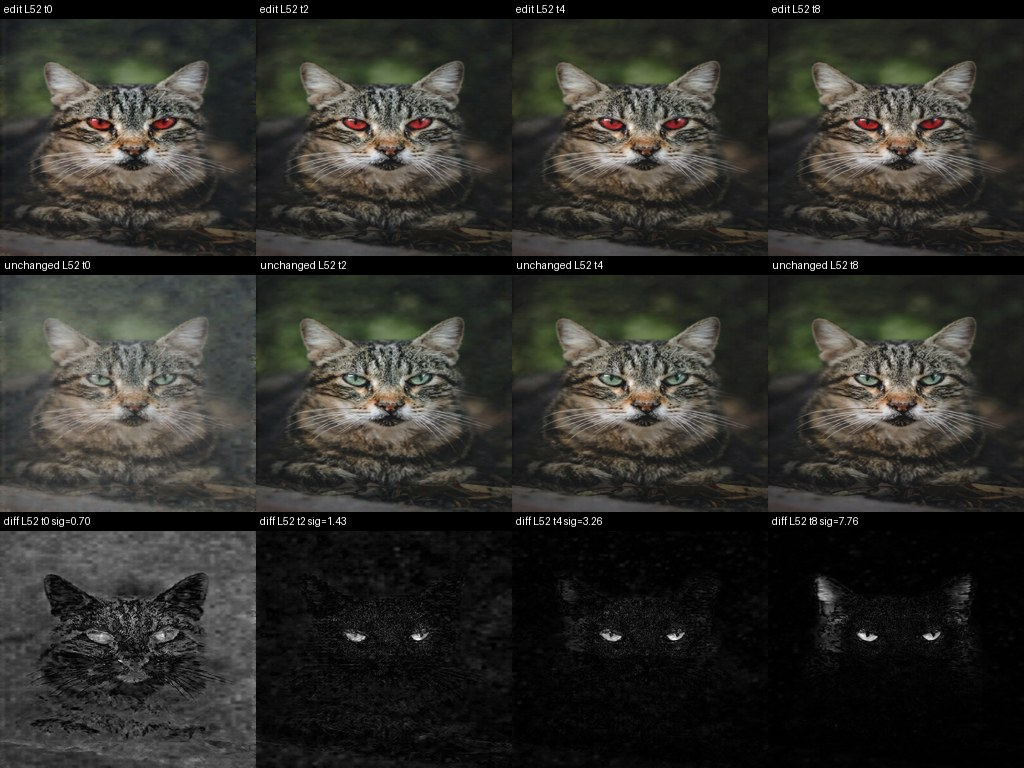
\includegraphics[width=0.98\textwidth]{figs/fig14_diff_lens/fig14_diff_lens.jpg}
  \caption{A differential lens applied to \emph{color\_eyes} (``change
  the cat's green eyes to red eyes''), decoded at L52 through the
  frozen K1 dictionaries of Figure~\ref{fig:tunedlens}. Top: the edit
  run's internal image already shows red eyes at $t{=}0$ and stays red
  throughout -- content is present early. Middle: the ``keep the image
  unchanged'' control's internal image keeps the source's green eyes at
  every step -- a faithful no-op. Bottom: the differential
  $D=|\text{edit}-\text{unchanged}|$ is a diffuse gray field over the
  whole face at $t{=}0$ ($\mathrm{sig}=0.70$, at the chance floor), and
  condenses monotonically into two glowing eyes in the dark by $t{=}8$
  ($\mathrm{sig}=7.76$, the sharpest concentration measured anywhere in
  this paper) -- content presence and separation are two different
  quantities.}
  \label{fig:difflens}
\end{figure*}

Figure~\ref{fig:difflens} shows this directly for \emph{color\_eyes}.
The onset curve at L52 (top row: edit; middle row: control; bottom row:
$D$) makes both halves of the claim visible in the same figure: the
top row already contains the edit at $t{=}0$, and the bottom row is not yet
localized at $t{=}0$ but sharpens every step after.

\textbf{A family signature: how fast the plan concentrates.} The onset
curve above ($\mathrm{sig}$ at L52, $t{=}0,2,4,8$) differs by family in
a way that recapitulates \S\ref{sec:families}'s two-axis law on a new
axis. Color edits concentrate fastest and hardest: eyes
$0.70\to1.43\to3.26\to7.76$, tree $1.30\to2.51\to3.05\to3.17$. The
invention edit starts at an exact chance floor and gathers slowly:
runner $0.91\to1.55\to2.27\to3.22$. A style edit (\emph{style\_ink},
``turn the photo into a Chinese ink painting'') stays nearly flat and
never concentrates: $1.95\to1.61\to1.67\to1.68$, and its Gini
($0.23$--$0.34$) is the lowest of any case we measured in this
paper -- a global plan has no single locus to concentrate onto, unlike
an object edit's local one.

\textbf{Bonus finding: the model cannot ``do nothing.''} Our first
differential run, \emph{car\_red} (the flat vector-art scene of
\S\ref{sec:tunedlens}), failed its own control: asked to ``keep the
image unchanged,'' the model instead cut the car out and rendered the
sky, road, and buildings as a transparent-PNG checkerboard -- a
training-data prior (transparent asset renderings) overriding an
explicit no-op instruction, while the edit run's own output stayed a
perfect red car on an intact scene. Every $\mathrm{loc}$/$\mathrm{sig}$/
Gini/$R^2$ number computed against this corrupted control is an
artifact of a broken ground truth, not a finding, and we discard the
case entirely rather than report it; the two color cases above (a
salvage run on natural photographs, which do pass the control-fidelity
check of \S\ref{sec:previewlever} below) supply the color-family
evidence instead. The lesson generalizes: any differential design needs
a control-fidelity gate \emph{before} its numbers are trusted, a
discipline \S\ref{sec:previewlever} applies as a standing check.

\subsection{A preview lever: reading the edit at 15\% NFE}\label{sec:previewlever}

If the differential above already carries the edit's spatial
footprint, does it carry it early enough in the 20-step trajectory to
be useful before a run finishes? We test this at $t{=}2$ -- the third
of 20 steps, $\approx$15\% of the run's forward passes -- on a narrower
$\{\text{L44},\text{L52}\}\times\{t{=}0,t{=}2\}$ grid, across a 10-case,
5-family battery of natural photographs (two source images per family:
color, object-removal, object-addition, background-replacement, style;
\texttt{runs/k4\_preview\_lever}). Every differential design needs the
control-fidelity discipline \S\ref{sec:difflens}'s bonus finding
demanded: before trusting any number, we gate each case on whether the
unchanged run's \emph{final} output actually matches the source
(grayscale Pearson $r$ against the source image, threshold $0.85$). All
10 cases pass ($r\in[0.856, 0.999]$); the one borderline case
(\emph{add\_ladybug}, $r=0.856$) is texture divergence in a
bokeh-dense scene under visual inspection, not a structural failure
like \emph{car\_red}'s.

\textbf{The preview is already informative at $t{=}2$.} Median IoU
between $D_{\text{L52},t2}$'s own top-10\% mass and the ground-truth
region $R$ is $0.33$ across the 10 cases -- $6.6\times$ the
$\approx$0.05 chance level -- ranging $0.13$--$0.81$
(\emph{remove\_duckfloat} highest). Every one of the 10 cases improves
from $t{=}0$ to $t{=}2$ ($10/10$, exceeding the pre-registered
$\ge$80\%). And the global/local distinction is already legible: the
two style cases (\emph{style\_ink}, \emph{style\_chibi}) rank lowest
and second-lowest in Gini($\text{L52},t2$) at $0.229$ and $0.250$, a
clear gap below the third-lowest case's $0.343$ -- exactly the ranking
\S\ref{sec:difflens}'s family-signature curve predicts.

\textbf{Target size, not onset family, drives the absolute preview
score -- a sixth documented failure-mode instance, and the first that
does not implicate CLIP at all.} We pre-registered that
addition/invention cases -- whose onset is delayed
(\S\ref{sec:when}, \S\ref{sec:difflens}) -- would rank lowest in
preview quality, on the reasoning that a differential that has not yet
localized cannot preview well. The ranking is not clean: the two
addition cases place \#2 and \#4 of 8 spatial cases by IoU (and
\#2/\#3 by a threshold-free AUROC re-analysis), and the single lowest
score on both metrics belongs to \emph{color\_eyes} -- the same case
Figure~\ref{fig:difflens} shows previews \emph{best} to the eye. The
mechanism is the ground-truth definition itself: $R$ is fixed at the
top-10\% of pixels regardless of how large the true edit is, so a
genuinely tiny edit (the cat's two eyes) gets an $R$ padded roughly
$10\times$ by collateral fur divergence, and every metric computed
against that inflated mask reads a precise preview as a poor one. Once
target size is controlled for by looking only at non-tiny targets, the
predicted ordering re-emerges: \emph{add\_runner}'s AUROC of $0.607$ is
the worst score among them. This is the sixth documented instance in
this paper of a quantitative readout diverging from the visual truth
(\S\ref{sec:limits} catalogs the first five, all CLIP) -- and the first
where the culprit is not CLIP but the mask that defines ground truth
for a purely geometric metric.

\begin{figure}[t]
  \centering
  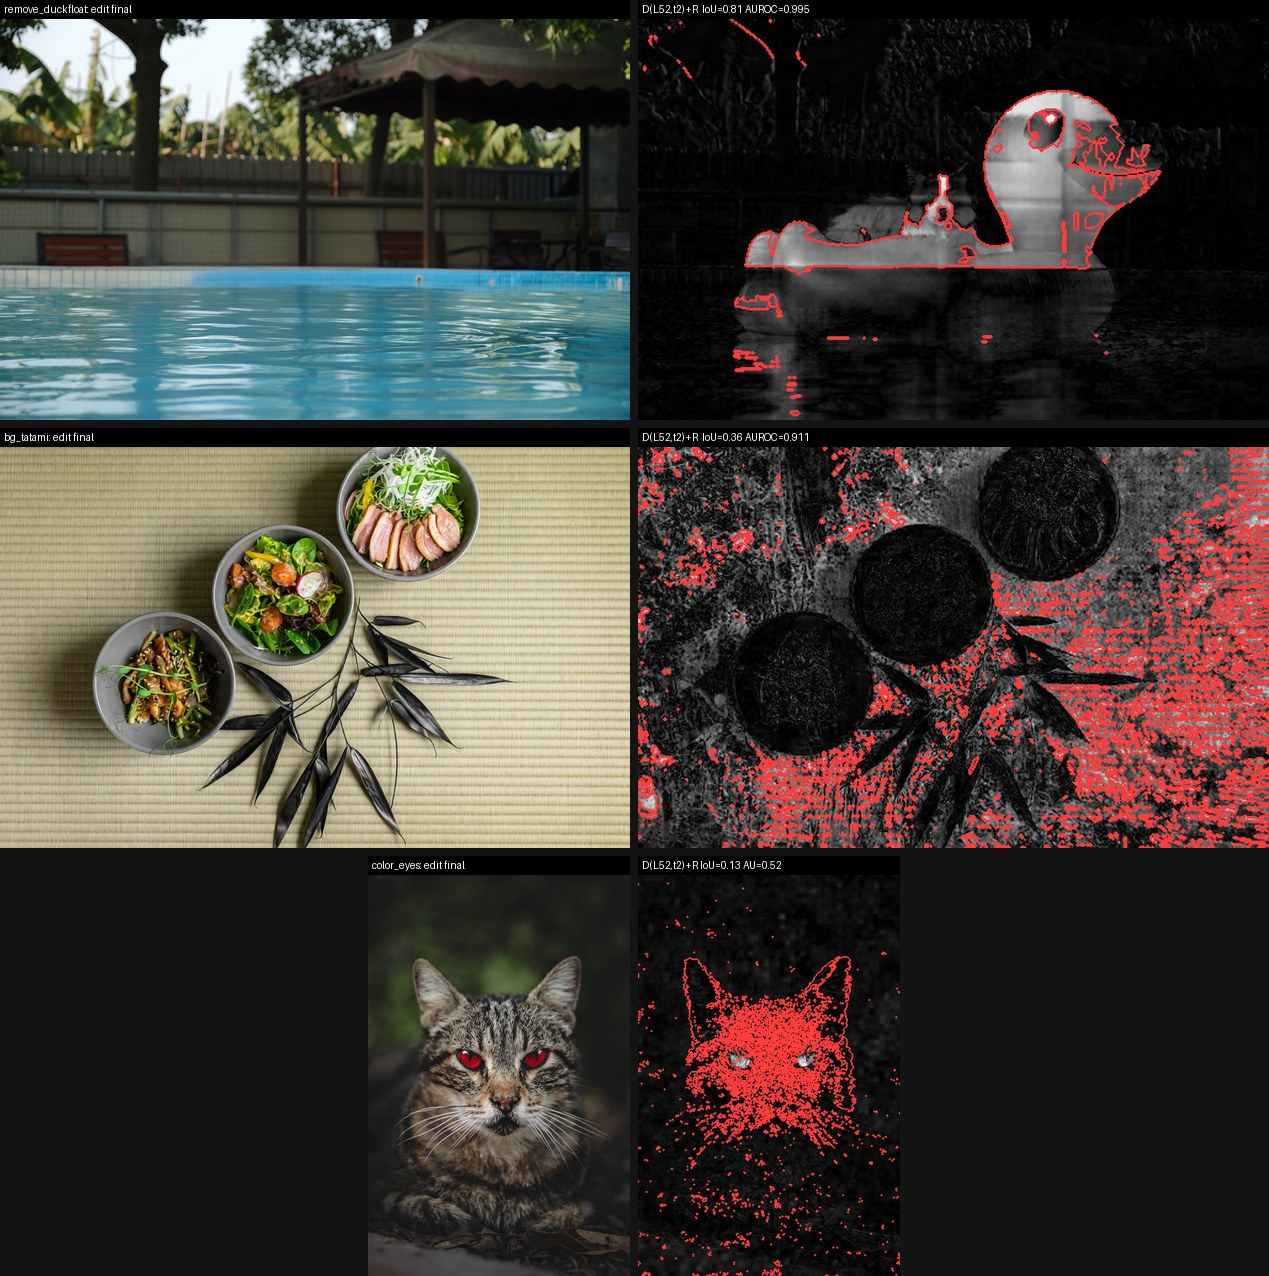
\includegraphics[width=\columnwidth]{figs/fig15_preview_lever/fig15_preview_lever.jpg}
  \caption{The differential lens as a $t{=}2$ ($\approx$15\% NFE)
  preview lever: three of the ten-case battery
  (\S\ref{sec:previewlever}). Left: each case's final edited output.
  Right: $D_{\text{L52},t2}$ (grayscale) with the ground-truth edit
  region $R$'s boundary overlaid in red. \emph{remove\_duckfloat}: the
  whole object slated for removal lights up as a duck-shaped ghost (IoU
  $0.81$, AUROC $0.995$). \emph{bg\_tatami}: a keep-vs-replace
  segmentation emerges unsupervised -- the three food bowls the prompt
  asks to preserve stay dark against a bright to-be-replaced background.
  \emph{color\_eyes}: two glowing eyes again, at only 15\% of the
  denoising trajectory -- visually the sharpest preview in the battery
  despite the lowest IoU/AUROC, because the fixed top-10\%
  ground-truth mask $R$ is padded roughly $10\times$ by collateral fur
  divergence around this tiny true edit (a metric artifact, not a
  preview failure).}
  \label{fig:previewlever}
\end{figure}

\textbf{The qualitative payoff, and the lever.} Figure~\ref{fig:previewlever}
shows three of the ten $t{=}2$ previews next to their edit's final
output; all 10 cases are qualitatively correct under visual inspection
at $t{=}2$. Because the unchanged control's capture does not depend on
the edit prompt at all, it can be computed once per source image and
cached. Previewing where and how large a \emph{candidate} edit will
land then costs only the handful of denoising steps needed to reach
$t{=}2$ (three forward passes, plus one frozen-dictionary decode)
rather than a full 20-step run -- a training-free way to triage many
candidate edit prompts against one image before committing to any of
them.

\subsection{Instruction injection: where the edit prompt is
consumed}\label{sec:injection}

\begin{table}[t]
\centering
\small
\begin{tabular}{lcccc}
\toprule
text cut at & $P(\text{red})$ & $P(\text{blue})$ & fid. in & fid. out \\
\midrule
L0--11  & 0.321 & 0.074 & 92.4 & 70.1 \\
L12--23 & 0.028 & 0.962 & 60.0 & 34.9 \\
L24--35 & 0.366 & 0.573 & 81.3 & 49.5 \\
L36--47 & 0.993 & 0.006 & 41.8 & 23.9 \\
L48--59 & 0.919 & 0.068 &  9.8 &  4.1 \\
all (0--59) & 0.014 & 0.976 & 62.0 &  4.0 \\
\bottomrule
\end{tabular}
\caption{Zeroing the \emph{text} stream (encoder\_hidden\_states) in only
the stated layer band, \emph{car\_red}, all 20 steps, both CFG passes.
Fidelity in/out are mean absolute pixel difference vs.\ the unablated
(red) baseline, inside/outside the car bounding box (data:
\texttt{runs/g3\_injection/summary.json}).}
\label{tab:injection}
\end{table}

The depth lens and explicit-prompt probe show color information is
linearly available by layer 6; neither tells us when the text-conditioned \emph{instruction}
itself is actually consumed by the image stream, as opposed to being
available but unused. We test this directly by zeroing only the
\emph{text}-stream tokens (\texttt{encoder\_hidden\_states}, never the
image stream) within a single layer band at a time, leaving every other
layer's text access untouched, and reading out the same car-region CLIP
scores used throughout \S\ref{sec:causal}--\S\ref{sec:swap}
(Table~\ref{tab:injection}).

\textbf{Injection is complete well before the translation band.} Cutting
text access only at L36--47 barely dents the edit ($P(\text{red})=0.993$,
though with non-trivial collateral cost to the rest of the scene, fidelity
outside $=23.9$); cutting it only at L48--59 is closer still to the
unablated baseline \emph{and} the cleanest of any band we tested
(fidelity outside $=4.1$, roughly $6\times$ better than L36--47's $23.9$).
Both results say the same thing: whatever the network needs from the text
stream to execute "turn the car red," it has already extracted by layer
36, so removing text access afterward changes almost nothing. This lines
up with \S\ref{sec:mechanism}'s probe result: if requested color is
already linearly readable by layer 6, the instruction cannot still be
waiting to be injected forty layers later.

\textbf{Injection itself is early and, unlike the later bands, not
optional.} Cutting text access at L0--11 or at L24--35 is destructive in a
qualitatively different way: both the car region \emph{and} the rest of
the scene are damaged (fidelity outside $70.1$ and $49.5$ respectively,
each far worse than any other band), and neither produces a clean
alternative reading. L0--11's output is not simply "wrong color": its
$P(\text{red})=0.321$ sits alongside a majority score for neither red nor
the source's blue, consistent with a genuinely garbled image rather than
a graceful fallback. These bands are not just carrying the instruction
forward; they are doing fusion work the rest of the network depends on to
render \emph{anything} coherent, edited or not. L12--23 is intermediate
(fidelity outside $34.9$): a cleaner, if still somewhat degraded, "ignore"
result. This is consistent with, and sharpens, \S\ref{sec:mechanism}'s
finding that requested color is linearly readable by layer 6: the instruction
must already be fused into the image stream within the first 11 blocks
for that linear signal to exist, and Table~\ref{tab:injection}
shows exactly why L0--11 cannot be spared.

\textbf{Cutting text access everywhere gives the cleanest possible
fallback.} Removing the text stream at every layer (\texttt{all}) does not
compound the mid-band damage above -- it instead produces the paper's
cleanest non-edit: a coherent reconstruction that ignores the instruction
entirely ($P(\text{blue})=0.976$, fidelity outside $=4.0$, on par with the
best-behaved partial cut). A network that never had text access at all
falls back cleanly to the source; a network that had it only \emph{before}
an intervening blackout (L0--11, L24--35) sometimes cannot recover
cleanly. Consistent with the mid-stack complementary-color code of
\S\ref{sec:depth}--\S\ref{sec:mechanism} (mechanized directly as a
tuned-lens anti-image in \S\ref{sec:tunedlens}), both the all-layers cut
and the L12--23-only cut land on the same "wrong" color, blue, rather
than a generic corruption -- an echo of the same sign-convention
structure this paper keeps finding, now produced by denying the network
its instruction rather than by mis-decoding an intermediate layer.
\subsection{Whole-token ablation as a failed localization test}\label{sec:causal}

\begin{figure*}[t]
  \centering
  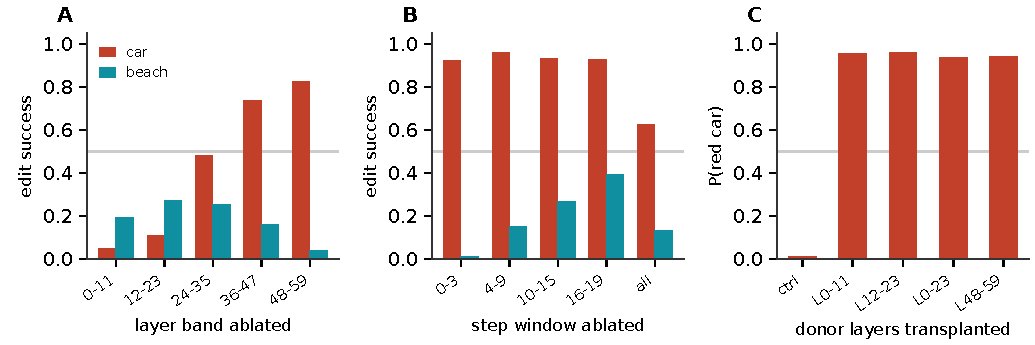
\includegraphics[width=0.98\textwidth]{figs/fig6_causality/fig6_causality.pdf}
  \caption{Historical whole-token stress tests and transplant.
  \textbf{A--B}: zero-overwrite scores are retained as a methodological
  negative; exact-region re-audit shows the edited tokens are driven
  off-manifold, so these panels cannot localize fine-grained necessity.
  \textbf{C}: transplanting a donor \emph{car\_red} state into a
  \emph{car\_green} recipient at any tested band is sufficient to move
  the output toward red.}
  \label{fig:causal}
\end{figure*}

This experiment was originally designed to ask whether readable layers
were causally necessary, using layer-band and step-window zero-overwrite
on target-grid tokens. The intended interpretation failed a later audit.
The intervention removes the entire residual token across many layers,
not a specific readable direction, and drives the edited region
off-manifold.

\textbf{Why the apparent layer profile is invalid.} The original margin
crop scored \emph{car\_red} at $0.049$ after L0--11 overwrite and $0.826$
after L48--59 overwrite. Exact-region crops reveal that both overwritten
regions are noise; the high late-band score comes from unablated red-car
pixels included by the expanded scoring margin. Mean replacement removes
that leakage-based contrast and collapses both bands. The analogous
\emph{beach\_background} comparisons are also dominated by destructive
whole-region effects. We therefore retain the numbers and images as a
failed localization attempt, not evidence that one layer band is
necessary or dispensable.

\textbf{Step windows.} Zeroing a 4--6 step window at 4 mid layers
($\ell\in\{12,24,36,48\}$) barely dents \emph{car\_red} regardless of
\emph{which} window is chosen ($0.92$--$0.96$ across all four
non-overlapping windows). \emph{beach\_background}
inverts this: ablating the earliest window (steps 0--3) is destructive
($0.014$) and the damage decreases roughly monotonically the later the
ablated window is (steps 16--19: $0.394$); ablating the same 4 layers
across \emph{all} 20 steps is worse still for both cases than any single
window ($0.627$ car, $0.134$ beach; Figure~\ref{fig:causal}B). These are
descriptive recovery profiles under a severe perturbation, not a
fine-grained causal map.

\textbf{Condition-token access.} Zeroing only the condition-image
tokens (never the target tokens) isolates how much the model needs to
keep re-consulting the source image, as opposed to having already
copied what it needs into the target stream. Table~\ref{tab:condtok}
shows that for \emph{car\_red}, even zeroing condition tokens at
\emph{every} layer barely dents the color score ($P(\text{red
car})=0.97$) -- but wrecks everything outside the car region
(\texttt{fidelity\_outside}, mean-squared pixel error against the
unablated baseline, jumps by more than an order of magnitude vs.\ the
layer-band ablations above). Cutting condition access only in the
\emph{early} half of the stack (layers 0--29) is worse for scene
fidelity than cutting only the late half (layers 30--59). This shows
that the stress test disrupts source-scene grounding; it does not isolate
the necessity of a particular edit representation.

\begin{table}[t]
\centering
\small
\begin{tabular}{lcc}
\toprule
condition tokens zeroed at & $P(\text{red car})$ & fidelity outside \\
\midrule
all layers (0--59)   & 0.972 & 61.5 \\
early half (0--29)   & 0.964 & 79.4 \\
late half (30--59)   & 0.991 & 57.5 \\
\bottomrule
\end{tabular}
\caption{Zeroing condition-image tokens only (target tokens untouched),
\emph{car\_red}, all 20 steps. Fidelity outside is mean-squared pixel
error vs.\ the unablated baseline, restricted to pixels outside the car
bounding box (data: \texttt{runs/a3\_summary.json}, \texttt{condtokens}
scan).}
\label{tab:condtok}
\end{table}
\subsection{Transplant establishes sufficiency}\label{sec:swap}

We take a \emph{car\_green} recipient run and, at each of four candidate donor
layer bands (L0--11, L12--23, L0--23, L48--59), overwrite its target
tokens in the car region with the corresponding tokens captured from a
\emph{car\_red} donor run of the same seed and source image (transplant,
\S\ref{sec:interventions}). An unmodified control run of the recipient
scores $P(\text{red car})=0.011$ (it is, correctly, a green car). Every
one of the four transplants flips the output back toward red:
$0.954$ (L0--11), $0.959$ (L12--23), $0.938$ (L0--23), and, notably,
$0.940$ for \textbf{L48--59} (Figure~\ref{fig:causal}C). The donor
representation is therefore sufficient to install the edit from every
tested band. This conclusion does not depend on, or combine with, the
failed necessity interpretation above. A
content-specificity control confirms the red-flip is not just a generic
effect of overwriting L0--23 with \emph{any} donor activity: substituting
the recipient's car-region tokens with the \emph{same} red-car donor
run's tokens from a same-sized, same-layer-band \emph{background}-region
patch box (wrong content, right layer band and token count) does not
produce red. It produces a garbled result CLIP scores as "a blue car"
($0.991$), neither the recipient's original green nor the donor's red.
The transplant installs the edit only when the donor content actually
matches the recipient's car-region positions; it is not a generic
disruption that happens to read out as the donor's label.

\subsection{Steering: a dose-response confirmation}\label{sec:steer}
% NOTE-G: two further G-phase runs exist but are deliberately NOT
% incorporated in this pass (see paper/provenance.md "G-phase note"):
% runs/g2_boundary/ (denser L44-59 crossover sweep; sharpens, doesn't
% change, the snap-zone finding) and runs/g3_injection/ (per-layer-band
% text-conditioning injection; landed after final compile, needs its own
% controlled analysis -- headline: text at L36-47 alone suffices,
% P(red)=0.993).

\begin{figure}[t]
  \centering
  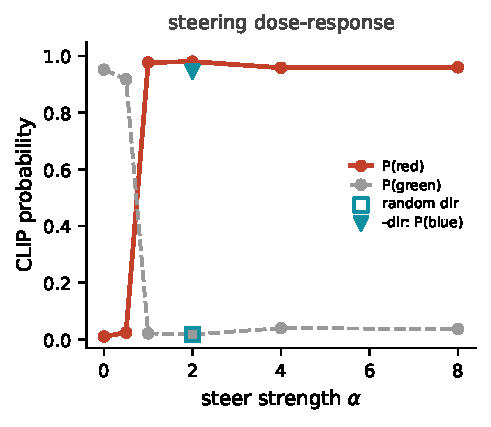
\includegraphics[width=\columnwidth]{figs/fig9_steering/fig9_steering.pdf}
  \caption{Steering the same \emph{car\_green} recipient toward red by
  adding $\alpha\, d_{\text{red}}$ (the probe direction from
  \S\ref{sec:mechanism}) to car-region rows at L6--23. $P(\text{red})$
  jumps sharply between $\alpha{=}0.5$ and $\alpha{=}1$ and saturates
  thereafter; a random direction at $\alpha{=}2$ (open square) barely
  moves either score; the negated direction at $\alpha{=}2$ (triangle)
  overshoots to \emph{blue}, not back to green.}
  \label{fig:steer}
\end{figure}

Transplant (\S\ref{sec:swap}) shows a donor's actual hidden state is
sufficient to install an edit; steering asks the narrower question of
whether a single \emph{direction} -- no donor forward pass, just a
stored vector -- is enough. Adding $\alpha\,d_{\text{red}}$ to the
\emph{car\_green} recipient's car-region rows at the same L6--23 band
used for transplant produces a sharp, sigmoidal dose-response
(Figure~\ref{fig:steer}): $P(\text{red car})$ is unmoved at
$\alpha{=}0.5$ ($0.024$, vs.\ $0.011$ unsteered), jumps to $0.977$ by
$\alpha{=}1$, and saturates around $0.96$--$0.98$ through
$\alpha{=}8$ -- consistent with crossing a comparatively sharp linear
decision boundary rather than a gradual blend. Two controls confirm
this is direction-specific, not a generic perturbation effect. A random
direction of the same norm at $\alpha{=}2$ (nearly orthogonal to
$d_{\text{red}}$, cosine similarity $0.006$) leaves the output at
$P(\text{red})=0.017$, statistically indistinguishable from unsteered.
The \emph{negated} direction, $-d_{\text{red}}$ at $\alpha{=}2$, does not
simply undo the edit back to green; it overshoots to
$P(\text{blue car})=0.945$ -- the same complementary-color pattern
\S\ref{sec:depth}--\S\ref{sec:mechanism} found in the mid-stack decode,
now produced by an active intervention rather than a passive readout.
As with transplant, this comes at a fidelity cost that grows with
$\alpha$ (\texttt{fidelity\_outside} rises from $0.95$ at
$\alpha{=}0.5$ to $33.4$ at $\alpha{=}8$): steering the same probe
direction identified in \S\ref{sec:mechanism} is a third, cheaper way
to move an edit, with the same necessity-independent sufficiency
property transplant showed, and the same practical fidelity/strength
tradeoff Figure~\ref{fig:apps} (right) showed for the global-CFG lever.
Layer- and timestep-specific steerability has also been observed for
contrastive concept directions in text-to-image DiTs
\citep{ohib2026conceptspaces}; our question here is narrower and
image-edit-specific: whether the direction preserves the spatial carrier on
which the attribute is written.

\paragraph{Self-correction: what ``flipped'' actually looks like.} The
numbers above were recorded from the dose curve and a three-way
forced-choice CLIP readout (red vs.\ blue vs.\ green car) -- a readout
that, by construction, cannot express ``no longer a car.'' Visually
re-auditing every steered output while extending steering across edit
families (\S\ref{sec:families}) showed that at effective doses the
steered region is not a recolored car but a flat red patch that
\emph{replaces} the car's geometry inside the steered rows (the green
nose and tail survive just outside them). The negated direction's
``blue'' is likewise a flat teal field with no car left in it. The dose
sharpness, the direction-specificity controls, and the hue semantics all
stand as stated; the implicit clean recolor-in-place reading does not.
The direction installs \emph{which} hue; it does not preserve what the
hue is painted on -- a distinction \S\ref{sec:families} turns into a
general rule, and a second instance (after the thumbnail episode of
\S\ref{sec:limits}) of a metric quietly standing in for looking at the
image.

\subsection{Attention-routing conservation audit}\label{sec:attentionaudit}

RESTORE diagnoses visual-token reduction by measuring the attention distortion
introduced by pruning and merging before proposing a matched correction
\citep{cho2026restore}. We borrow that experimental pattern, not its reduction
or calibration mechanism. On the fixed car case, we preregistered five seeds,
five layers, five denoising steps, three query groups, and four key groups. A
side recorder recomputes conditional-pass joint attention after Q/K
normalization and RoPE while delegating the actual attention output unchanged;
all interventions remain symmetric across both CFG passes. Across 1,000
recorded cells, the four key-group masses sum to one within
$1.97\times10^{-6}$, and six historical seed-0 renders reproduce pixel-exactly.

\begin{figure*}[t]
  \centering
  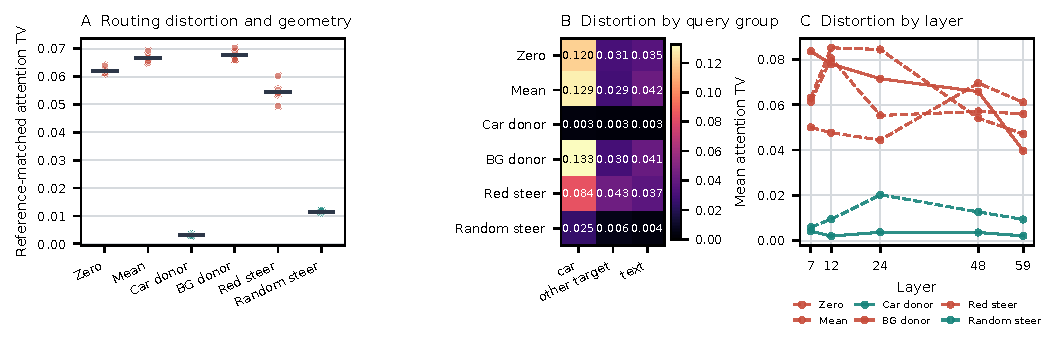
\includegraphics[width=0.98\textwidth]{figs/fig20_attention_conservation/fig20_attention_conservation.pdf}
  \caption{T11 attention-routing conservation audit. \textbf{A}: the
  preregistered reference-matched total-variation distortion for each of five
  seeds; bars mark condition means, teal marks geometry-coherent renders, and
  red marks incoherent renders. The destructive-minus-on-manifold contrast is
  positive in 5/5 seeds (mean $0.0356$, exact one-sided sign-flip
  $p{=}0.03125$). \textbf{B--C}: post-hoc decompositions by query group and
  layer; they do not alter the registered gate.}
  \label{fig:attentionaudit}
\end{figure*}

The content-matched car donor nearly reproduces the natural red-reference
routing (mean TV $0.0031$) and preserves a coherent car in 5/5 seeds. The
equal-size background donor is as distorted as zero/mean replacement (TV
$0.0677$) and destroys the region in 5/5, so transplant coherence is
content-specific rather than a generic overwrite effect. Red-direction
steering is the boundary case: it writes red in 5/5 but has high routing
distortion (TV $0.0546$) and produces a flat patch in 5/5. Thus the audit
supports attention-routing conservation as an explanation for the tested
coherent transplant and strengthens the carrier-bounded writability reading of
steering, consistent with the broader detection--intervention gap reported by
\citet{pegoraro2026look}. It does not make whole-token replacement a valid necessity test, nor
does it establish token reduction, speedup, architecture-general conservation,
or transfer of RESTORE's positional calibration.

\subsection{Applications}\label{sec:applications}

\begin{figure*}[t]
  \centering
  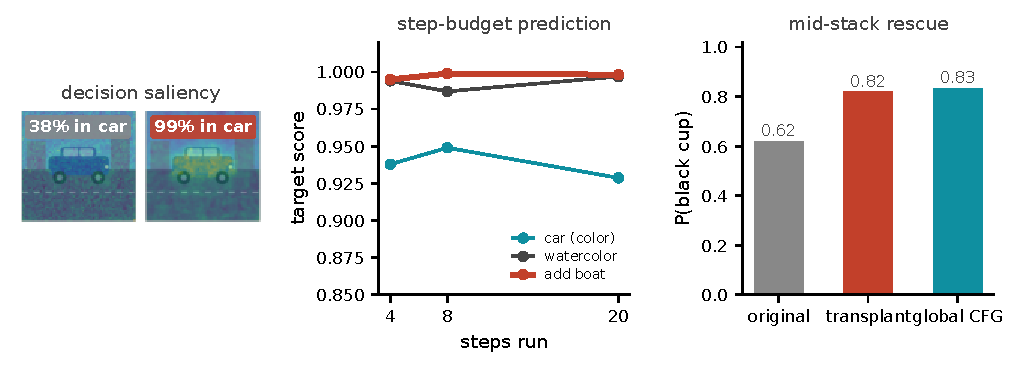
\includegraphics[width=0.98\textwidth]{figs/fig7_applications/fig7_applications.pdf}
  \caption{Three practical uses of the lens. Left: a saliency map built
  from the trained linear probe at the L12/$t$4 hero cell puts $99\%$ of
  its top-decile mass inside the car region, vs.\ $38\%$ for a raw
  magnitude heatmap at the same cell (chance level $19\%$). Center: three
  cases run at genuinely reduced step budgets (4, 8, 20 steps); the two
  early-saturating cases are already near their 20-step target score at
  4 steps, the delayed-onset case needs slightly more. Right: transplanting
  L6--23 hidden states from a stronger (CFG 7) run into a weaker (CFG 4)
  recipient rescues an under-strength edit about as well as simply
  raising the recipient's own guidance scale.}
  \label{fig:apps}
\end{figure*}

\textbf{Probe saliency.} A linear probe trained on the captured
hidden states (\S\ref{sec:mechanism}'s probe methodology, here trained
directly rather than cross-seed) gives us a per-patch importance score
"for free," by taking the magnitude of its gradient/weight contribution
at each patch position. At the L12/$t$4 hero cell, thresholding this
probe-derived saliency at its top decile puts $99.0\%$ of the selected
patches inside the car's bounding box (chance level, given the box
covers $19.4\%$ of the grid, is $19\%$); the raw activation-magnitude
heatmap at the identical layer/step -- the naive diagnostic in
\S\ref{sec:massive} -- puts only $38.3\%$ of its top decile inside the
same box. A probe-derived saliency map is a substantially better "where
is the model actually deciding this" visualization than a magnitude
heatmap, at negligible extra cost once the probe exists.

\textbf{Step-budget prediction.} \S\ref{sec:when} showed semantic readouts saturate at
different steps depending on content. This suggests a practical
question: for a given edit, how few denoising steps can we actually
afford? We re-ran three cases (\emph{color\_car}, \emph{style\_watercolor},
\emph{add\_boat}) with genuinely reduced step budgets (4 and 8 steps,
each with its own noise schedule, not a truncation of the 20-step
trajectory) and compared the target CLIP score to the 20-step
reference. The two early-saturating cases are already within $0.02$ of
their reference score at 4 steps (color\_car: $0.938$ vs.\ $0.929$;
style\_watercolor: $0.994$ vs.\ $0.997$); \emph{add\_boat}, whose
saturation step is latest in our battery, is slightly behind at 4 steps
($0.995$) but closes the gap by 8 ($0.999$ vs.\ $0.998$). We flag one
important caveat here: matching CLIP scores does not mean matching
images -- \emph{color\_car} at 4 steps still differs from the 20-step
reference by a mean-squared pixel error an order of magnitude larger
than at 8 steps ($290.7$ vs.\ $83.3$), so a CLIP-score-based step-budget
recommendation should be read as "the requested edit is present," not
"the image is pixel-identical to a full run."

\textbf{Mid-stack transplant rescue.} If an edit comes out under-strength
at the model's default guidance scale, \S\ref{sec:swap}'s transplant
machinery gives a second lever besides simply increasing CFG. For
\emph{color\_cup} ("turn the cup black") at CFG 4, the baseline cropped
$P(\text{black cup})$ is $0.619$. Raising CFG alone to 7 (a purely
sampling-side change, no hidden-state intervention) brings this to
$0.834$. Transplanting hidden states at layers 6--23, all steps, from a
same-seed CFG-7 donor run into the CFG-4 recipient reaches $0.819$ --
within $0.015$ of the global-CFG result, while changing the fidelity
outside the cup region less (mean-squared pixel error $0.805$ vs.\
$1.192$ for the CFG-7 alternative). The transplant is a more surgical
lever: it strengthens the specific edit without also amplifying
guidance everywhere else in the image.

\subsection{A methodological caution: massive activations}\label{sec:massive}

Everything above reads out a \emph{semantic} score by decoding through
the frozen head or a trained probe. A much cheaper diagnostic -- one we
used ourselves in early exploration, and one we suspect others will
reach for first -- is to just look at the raw per-patch activation
\emph{magnitude} (L2 norm) at a given layer/step and treat high-norm
patches as "important." This is unreliable at depth. Very deep layers
(L54--L59) develop a handful of \emph{massive activations}: a small
number of channels (\eg{}, in our capture, one recurring outlier channel
around index 673) and a small number of patches whose norm is orders of
magnitude larger than the rest of the grid -- at L59 we measured
patch-level absmax on the order of $10^9$, while the bulk of patches sit
around $10^5$--$10^7$. A raw-norm heatmap at these layers is dominated
by these few outliers and visually washes out any spatial structure.
We also observed that which case looks "hotter" by this measure does not
track edit difficulty or success in any way we could interpret
(\emph{beach\_background}'s raw-magnitude norms at deep layers are
larger than \emph{car\_red}'s, despite both edits succeeding). Mid-depth
layers (roughly L12--L36) do not show this pathology and are where we
default to for any raw-magnitude visualization, including the naive
comparison point in Figure~\ref{fig:apps} (left). The lesson we take
from this is narrow but important: a semantic readout (frozen-head
decode, or a trained probe as in \S\ref{sec:applications}) is not
optional plumbing on top of a magnitude heatmap -- at the layers where
edit semantics are legible, magnitude alone is actively
misleading.

This observation is not a novelty claim about the existence of massive
activations. \citet{gan2026massive} independently study them across multiple
DiTs and show that disrupting them primarily affects local-detail synthesis
rather than global semantics. Our narrower caution is measurement-specific:
in this editor, raw magnitude is therefore a poor proxy for the semantic edit
signal that the lens is intended to read.

\subsection{Does this generalize? A cross-model replication}\label{sec:generalize}

\begin{figure*}[t]
  \centering
  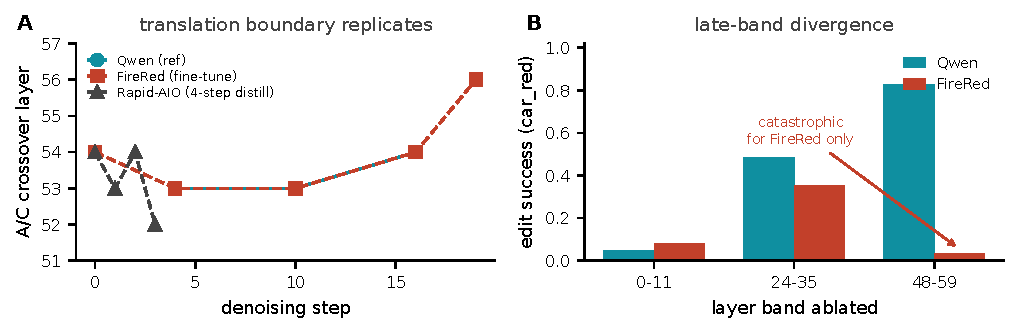
\includegraphics[width=0.98\textwidth]{figs/fig11_replication/fig11_replication.pdf}
  \caption{Cross-model replication of the core measurements.
  \textbf{A}: the A/C decode-crossover layer (\S\ref{sec:mechanism}) for
  \model{} (reference), an independently fine-tuned checkpoint
  (FireRed-Image-Edit-1.1), and a 4-step distilled merge (Rapid-AIO), all
  clustered within L52--56. \textbf{B}: layer-band zero-ablation edit
  scores for \emph{car\_red}, \model{} vs.\ FireRed. Their divergence is
  retained as evidence that this off-manifold stress test is not a
  transferable necessity measure.}
  \label{fig:replication}
\end{figure*}

Most mechanistic findings so far concern one checkpoint, \model{}. We
test which measurements persist within its model lineage by re-running
the depth-lens crossover, explicit-prompt probe, and stress test on two further
checkpoints that share \model{}'s transformer classes: FireRed-Image-Edit-1.1,
an independently fine-tuned checkpoint, and a 4-step distilled merge
(Rapid-AIO) built on the same shell.

\textbf{The boundary and explicit-prompt readability replicate.} FireRed's
A/C decode crossover (\S\ref{sec:mechanism}) lands at L53--56 across steps
0, 4, 10, 16, 19 (L54, 53, 53, 54, 56); the 4-step Rapid-AIO merge's
crossover across its own steps 0--3 is L52--54 (L54, 53, 54, 52) -- both
tightly clustered around the same L52--54 band \S\ref{sec:mechanism}
measured for \model{}. FireRed's cross-seed probe accuracy at L6, $t{=}4$
is $0.852$ (vs.\ \model{}'s $0.883$) and dips to $0.69$--$0.70$ at L59
across steps (vs.\ \model{}'s $0.68$--$0.70$) -- the same flat-then-dip
shape, from an independent fine-tune. Rapid-AIO's color readout saturates
immediately in its compressed 4-step schedule ($P(\text{red})@\text{L59}
= 0.955$ at $t{=}0$, staying flat and high through $t{=}3$), the same
early-saturation pattern \S\ref{sec:when} found for \model{}'s 20-step
color edits.

\textbf{The requested-color direction transfers within the lineage.} A probe trained on one
model's activations and evaluated on the other's -- held out by
\emph{model}, not merely by seed -- reaches $0.840$ (train \model{}, test
FireRed) and $0.917$ (train FireRed, test \model{}) accuracy, both close
to each model's own within-model, cross-seed accuracy ($0.877$ \model{},
$0.816$ FireRed). The two models' L12/$t$4 probe directions, moreover,
have cosine similarity $0.833$. Requested color is represented in
nearly the same direction of the shared 3072-dimensional hidden space
across an independent fine-tune, not merely at the same layer index.

\textbf{The stress test diverges.} Zero-overwriting L0--11 is destructive
for both models ($0.049$ \model{}, $0.082$ FireRed), while L48--59 gives
$0.826$ on \model{} and $0.035$ on FireRed. Exact-region inspection shows
off-manifold corruption, and \S\ref{sec:causal} already invalidates the
high \model{} score as margin-crop leakage. The cross-model divergence
therefore reinforces the methodological conclusion: whole-token
zero-overwrite is not a stable necessity measure and supports no
architecture-level causal claim.

\begin{figure*}[t]
  \centering
  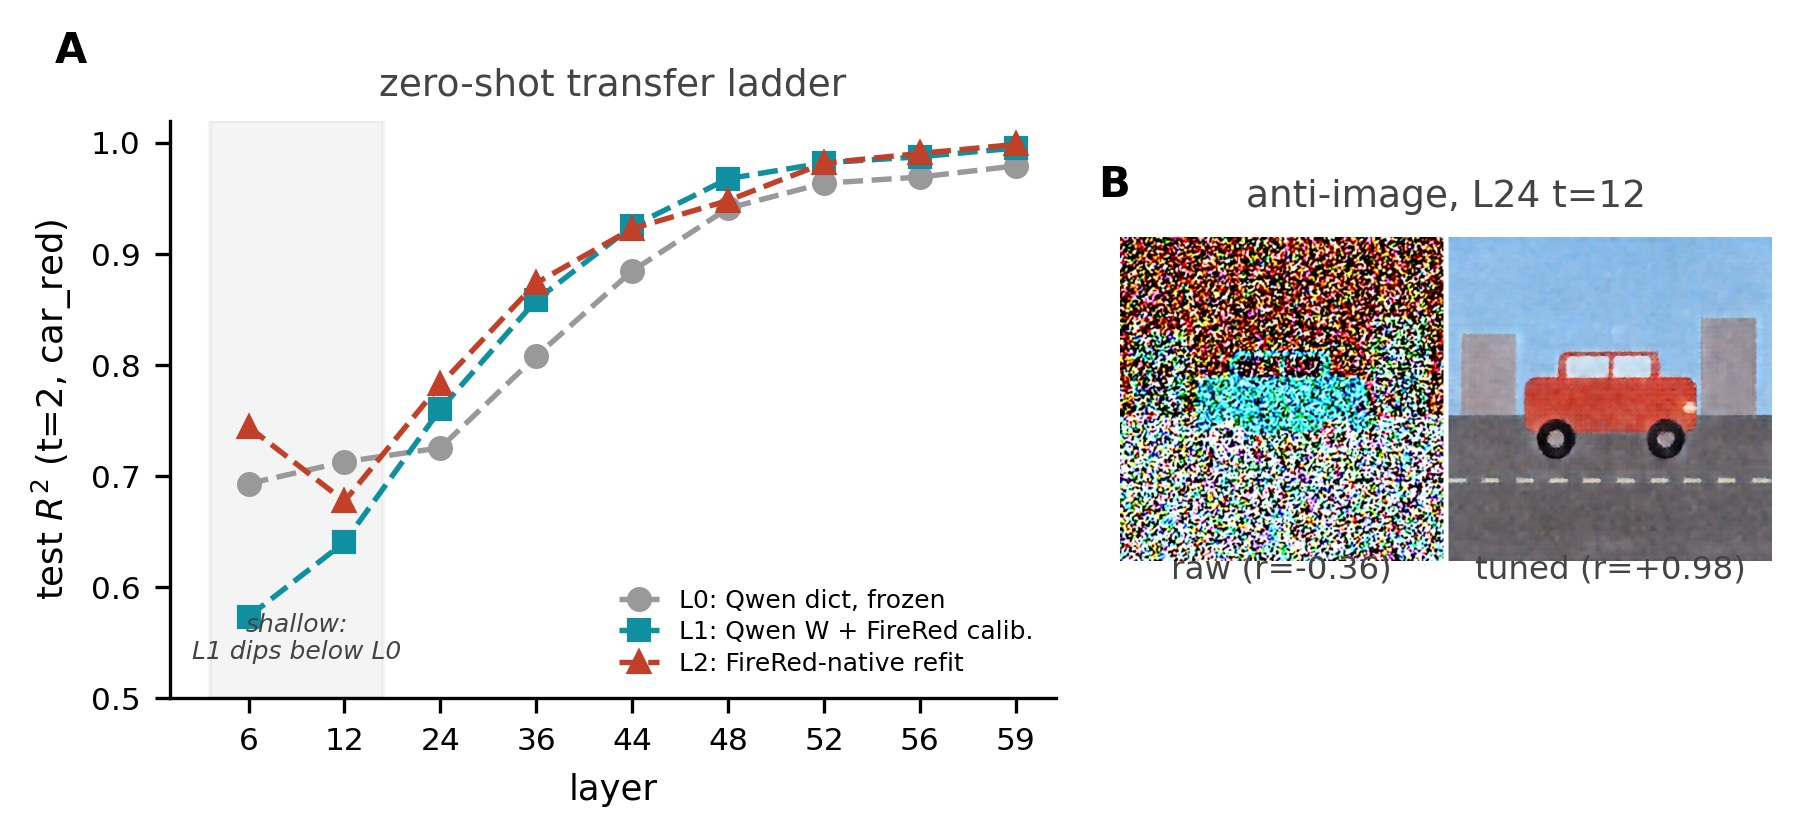
\includegraphics[width=0.98\textwidth]{figs/fig16_crossmodel_lens/fig16_crossmodel_lens.jpg}
  \caption{The lens toolchain transfers to FireRed-Image-Edit-1.1.
  \textbf{A}: test $R^2$ at $t{=}2$ across the 9 probed layers for the
  three-rung transfer ladder on held-out \emph{car\_red} -- L0 (\model{}
  translator dictionary $W$, fully frozen), L1 (same $W$, FireRed's own
  recalibration), L2 (FireRed-native refit of $W$ and calibration). At
  deep layers all three converge with L1$\approx$L2, showing $W$ itself
  needs no refitting; the shaded band marks L6/L12, the one region where
  L1 can dip below L0 (data: \texttt{ladder\_r2.json}). \textbf{B}: the
  anti-image replicates -- the same cell (L24, $t{=}12$) decoded by the
  raw frozen head (left) versus the native tuned lens (right): a cyan
  car under a red-brown sky versus the correct red car under blue sky,
  pixel-Pearson-vs-final $-0.36$ vs.\ $+0.98$ (data:
  \texttt{cells/\{raw,tuned\}\_L24\_t12.png}, \texttt{summary.json}).}
  \label{fig:crossmodel-lens}
\end{figure*}

\paragraph{The full lens toolchain, not just the probe, transfers.} The
replication above concerns the frozen-head boundary and a linear probe;
we separately ask whether this paper's newer toolchain -- the tuned
lens (\S\ref{sec:tunedlens}), its differential form
(\S\ref{sec:difflens}), and the $t{=}2$ preview lever
(\S\ref{sec:previewlever}) -- transfers with the same zero-code recipe,
on FireRed-Image-Edit-1.1. We refit \S\ref{sec:tunedlens}'s
per-(layer, step) translators natively on FireRed (identical
three-case training split, held-out \emph{car\_red}) and additionally
build a three-rung transfer ladder on that same held-out case:
\textbf{L0} decodes FireRed activations through the \model{} translator
weights $W$, frozen exactly as fit on \model{}; \textbf{L1} keeps that
same $W$ but substitutes FireRed's own fitted calibration
(mean/std/target-mean); \textbf{L2} refits both $W$ and calibration
natively on FireRed (the model used everywhere else in this section).
L1 and L2 therefore differ only in $W$; L0 and L1 differ only in
calibration. At the deep layers where the head-readable boundary lives
(L52, 56, 59), $R^2$ orders $\text{L0} \ll \text{L1} \approx \text{L2}$:
recalibrating a frozen \model{}-fit $W$ closes nearly all of the gap to
a fully native fit, and refitting $W$ itself buys almost nothing
further. At the final probed layer (L59) at \emph{car\_red}'s first step,
$R^2$ goes $0.943 \to 0.991 \to 0.997$ (L0$\to$L1$\to$L2) -- recalibration alone
recovers 89\% of the frozen-to-native gap at this cell. L1 sits
within $0.005$ of L2 at nearly every deep-layer cell, and on two of them
(L52 at $t{=}2, 16$) L1 fractionally \emph{exceeds} L2 -- the strongest
form of the claim, since it means refitting $W$ does not help at all.
We read this as the readout basis $W$ being an architecture-level
property, not a checkpoint-level one -- what a new checkpoint needs is
recalibration, not a new basis. The one honest caveat is at the
shallow layers L6/L12: at early steps ($t\le4$) L1 occasionally dips
\emph{below} L0 (\emph{e.g.}\ L6, $t{=}2$: $0.573$ vs.\ $0.693$) --
neither $W$ nor calibration transfers cleanly this shallow, and the
strict L0$\ll$L1$\approx$L2 ordering is a deep-layer phenomenon. A
bonus finding sits inside the same ladder: L0 -- the fully frozen
\model{} dictionary, never having seen a single FireRed activation --
already decodes a coherent, image-level grid at every probed layer,
$R^2 = 0.93$--$0.98$ at L52--59; the picture only turns slightly
yellower and grainier at early steps, exactly where L1/L2 pull ahead
(Figure~\ref{fig:crossmodel-lens}A). The ladder is not a single-case
anecdote: re-run on FireRed over the same six-case held-out battery
\S\ref{sec:tunedlens} used for family generality -- six captures,
zero refitting beyond the dictionaries already on disk -- every one
of the $108$ deep-layer cells ($6$ cases $\times$ L52/56/59
$\times$ $6$ steps) orders strictly
$\text{L0}<\text{L1}<\text{L2}$ with zero near-ties, and recalibration
recovers a median $89\%$ of the frozen-to-native gap. The frozen
dictionary's deep-layer $R^2$ never falls below $0.86$ on any case,
and \emph{style\_ink} -- the one family the translators never saw --
posts the second-highest frozen-dictionary floor of the six
($0.885$). All six cases pass the L59 self-consistency gate
bit-exactly, and visual inspection of all six three-rung strips
finds the rungs agreeing on content everywhere, L0 differing only in
texture noise. The one systematic soft spot is small: the six cells
whose gap recovery dips below $0.5$ all sit in the $t{=}4$ column
(absolute $R^2$ still ${\ge}0.97$ there).

Refit natively (L2 above), the tuned lens reproduces
\S\ref{sec:tunedlens}'s central claim verbatim: no hard affine
boundary across the full depth, including L6; at $t{=}0$ the same
depth-assembly sequence \S\ref{sec:tunedlens} found for \model{} --
ghost car at L24, dark silhouette at L36, formed at L44, red car at
L52 -- and test $R^2 = 0.970$--$0.999$ at L52 and above. The anti-image
replicates almost verbatim: the raw frozen head, applied mid-stack to
FireRed's own activations, decodes the same color-inverted scene
\S\ref{sec:tunedlens} found for \model{}, a cyan car under a
red-brown sky. Pixel Pearson correlation against the final frame runs
$-0.32$ to $-0.38$ at $t{=}12$ across L6--L48 (\model{}'s reference
value: $-0.40$), deepening to $-0.73$ by $t{=}16$; the tuned lens at
the identical cells is $+0.96$ or higher.
Figure~\ref{fig:crossmodel-lens}B shows one such cell directly (L24,
$t{=}12$): the raw decode is legible as a cyan car on a red-brown
ground once you know to look for it, while the tuned decode at the
same coordinates is the correct red car on blue sky.

\textbf{The differential law and the preview lever transfer, with one
rate correction.} Re-running the differential lens
(\S\ref{sec:difflens}) natively on two held-out FireRed cases --
\emph{color\_tree} ("turn the tree trunk black") and \emph{add\_runner}
("add a man running in sportswear on the road") -- after both pass the
control-fidelity gate ($r=0.933$ and $r=0.990$, both above the $0.85$
bar) reproduces early content visibility: both cases' internal image already
shows the edit at $t{=}0$, and localization (loc, at L52) rises
monotonically with step in both ($0.90\to0.97$ for \emph{color\_tree},
$0.29\to0.84$ for \emph{add\_runner}). The invention-family
floor-start law (\S\ref{sec:difflens}) holds exactly:
\emph{add\_runner}'s concentration statistic climbs from a near-floor
$1.66$ at $t{=}0$ through $2.75$ and $4.27$ to $5.42$ at $t{=}8$, the
same monotone-from-floor shape \S\ref{sec:difflens} reported for
\model{}. The color family's \emph{rate} does not transfer as cleanly:
\emph{color\_tree}'s concentration statistic already reaches $4.45$ --
near its own plateau ($4.85\to4.70\to4.76$ at later steps) -- at
$t{=}0$, rather than \model{}'s gradual $1.30\to3.17$ climb
(\S\ref{sec:difflens}). The qualitative law -- color edits separate
faster than invention edits -- holds; its \emph{onset rate} is a joint
property of the model and the edit family, not a model-independent
constant. The $t{=}2$ preview lever (\S\ref{sec:previewlever})
transfers on the same two cases: $\mathrm{IoU@top10}(\text{L52},
t{=}2) = 0.676$ (\emph{color\_tree}) and $0.217$ (\emph{add\_runner}),
both above the $0.15$ bar registered for this replication and well
above the $0.05$ chance level, with $\mathrm{IoU}(t{=}2) >
\mathrm{IoU}(t{=}0)$ in both cases ($0.610\to0.676$,
$0.142\to0.217$).

\textbf{Gates.} Every number above passed the same discipline this
paper insists on throughout: the L59 self-consistency gate is exact
(\texttt{max\_rel\_diff}$=0.0$ -- FireRed's \texttt{zero\_cond\_t=False}
temb path decodes bit-identically), and the "keep the image unchanged"
control passes fidelity ($r=0.933$/$0.990$) on both differential cases.

\S\ref{sec:tunedlens}--\S\ref{sec:previewlever}'s observations -- no hard
affine readability boundary, early content with gradual differential
separation, and a usable 15\%-NFE preview -- also reproduce on this one
fine-tuned checkpoint. The practical
recipe this buys: deploying the lens on a new checkpoint in the same
family does not require refitting the translator dictionary $W$ from
scratch -- freezing it and only recalibrating (or, at deep layers, not
even that) already gets most of the way there. As with the replication
above, this remains a single-held-out-case ladder on one independently
fine-tuned checkpoint that shares \model{}'s transformer classes. A
from-scratch, architecturally distinct DiT has only been tested for early
outcome prediction and selection, not the full lens toolchain.

\textbf{A larger shift still -- distillation, merging, and a different
sampler -- shows what the velocity-code dictionary is actually keyed
on.} FireRed and Rapid-AIO above (Figure~\ref{fig:replication}) are
independently trained but both keep \model{}'s 20-step schedule; we
push the same three-rung ladder (L0 frozen / L1 recalibrated / L2
native-refit) onto Rapid-AIO v23 -- a 4-step distilled, merged
community checkpoint of the same architecture, run under its
recommended ancestral/beta sampler -- where the noise schedule itself,
not only the weights, has moved. Because Rapid-AIO's four steps sit at
noise levels $\sigma$ that fall between \model{}'s twenty, each rung
must first choose which of the six captured \model{}-fit dictionary
entries to borrow; two rival choices -- nearest $\sigma$, or nearest
fractional schedule position -- agree everywhere except one column
($t{=}2$: Rapid $\sigma=0.290$ borrows the $\sigma=0.278$ entry under
$\sigma$-matching versus $\sigma=0.536$ under fraction-matching). At
every deep-layer cell in that column $\sigma$-matching wins (6/6,
median $+0.055$; 16/18 across all nine probed layers), with a clean
dose-response over the run: a $0.012$ $\sigma$-gap costs nothing,
$0.246$ costs ${\sim}0.05$ $R^2$, and the final step's $0.26$ gap is
catastrophic -- the dictionary is keyed to noise level, not schedule
position. Once steps are $\sigma$-matched, the frozen \model{}
dictionary sits at near-parity with a Rapid-AIO-native refit wherever
the dictionary has $\sigma$-coverage ($t{=}0$--$2$): deep $R^2$ runs
$0.927$--$0.995$ on both \emph{car\_red} and \emph{style\_ink} (the
family the translators never saw), 13 of 24 deep cells near-ties (a
few favoring the frozen dictionary) -- less damage from this much
larger distillation shift than the fine-tune shift above did to the
same cells. The one genuine failure is $\sigma$-\emph{coverage}, not
distillation: the final step ($\sigma=0.02$) falls outside the six
captured entries (nearest $\sigma=0.2735$), where the frozen dictionary
is negative-$R^2$, recalibration can make it worse ($-1.88$ for
\emph{style\_ink}), and even the Rapid-AIO-native refit reads reliably
only at the final block ($0.28$--$0.72$ at L52/56 vs.\
$0.98$--$0.99$ at L59). This
failure is invisible at the pixel level: $x_0=\text{latents}-\sigma v$
damps the velocity term to ${\sim}2\%$ of its scale at this $\sigma$,
so the worst cell (velocity $R^2=-1.88$) still decodes to a visually
clean ink painting; only the velocity-space $R^2$, not visual
inspection, detects this class of failure. Two of five pre-registered
predictions were refuted as literally stated, both for the same
reason: their thresholds were calibrated to the fine-tune ladder's gap
structure, which this $\sigma$-aligned shift does not reproduce -- a
$\ge0.85$ native-refit floor (met on 20/24 deep cells, all four misses
confined to the out-of-coverage final step) and a $\ge$60\% median
gap-recovery rate (actual median $0.529$, degenerate once 13/24 cells
have no gap left to recover, and negative where recalibrating a
wrong-$\sigma$ dictionary actively hurts).

\begin{figure*}[t]
  \centering
  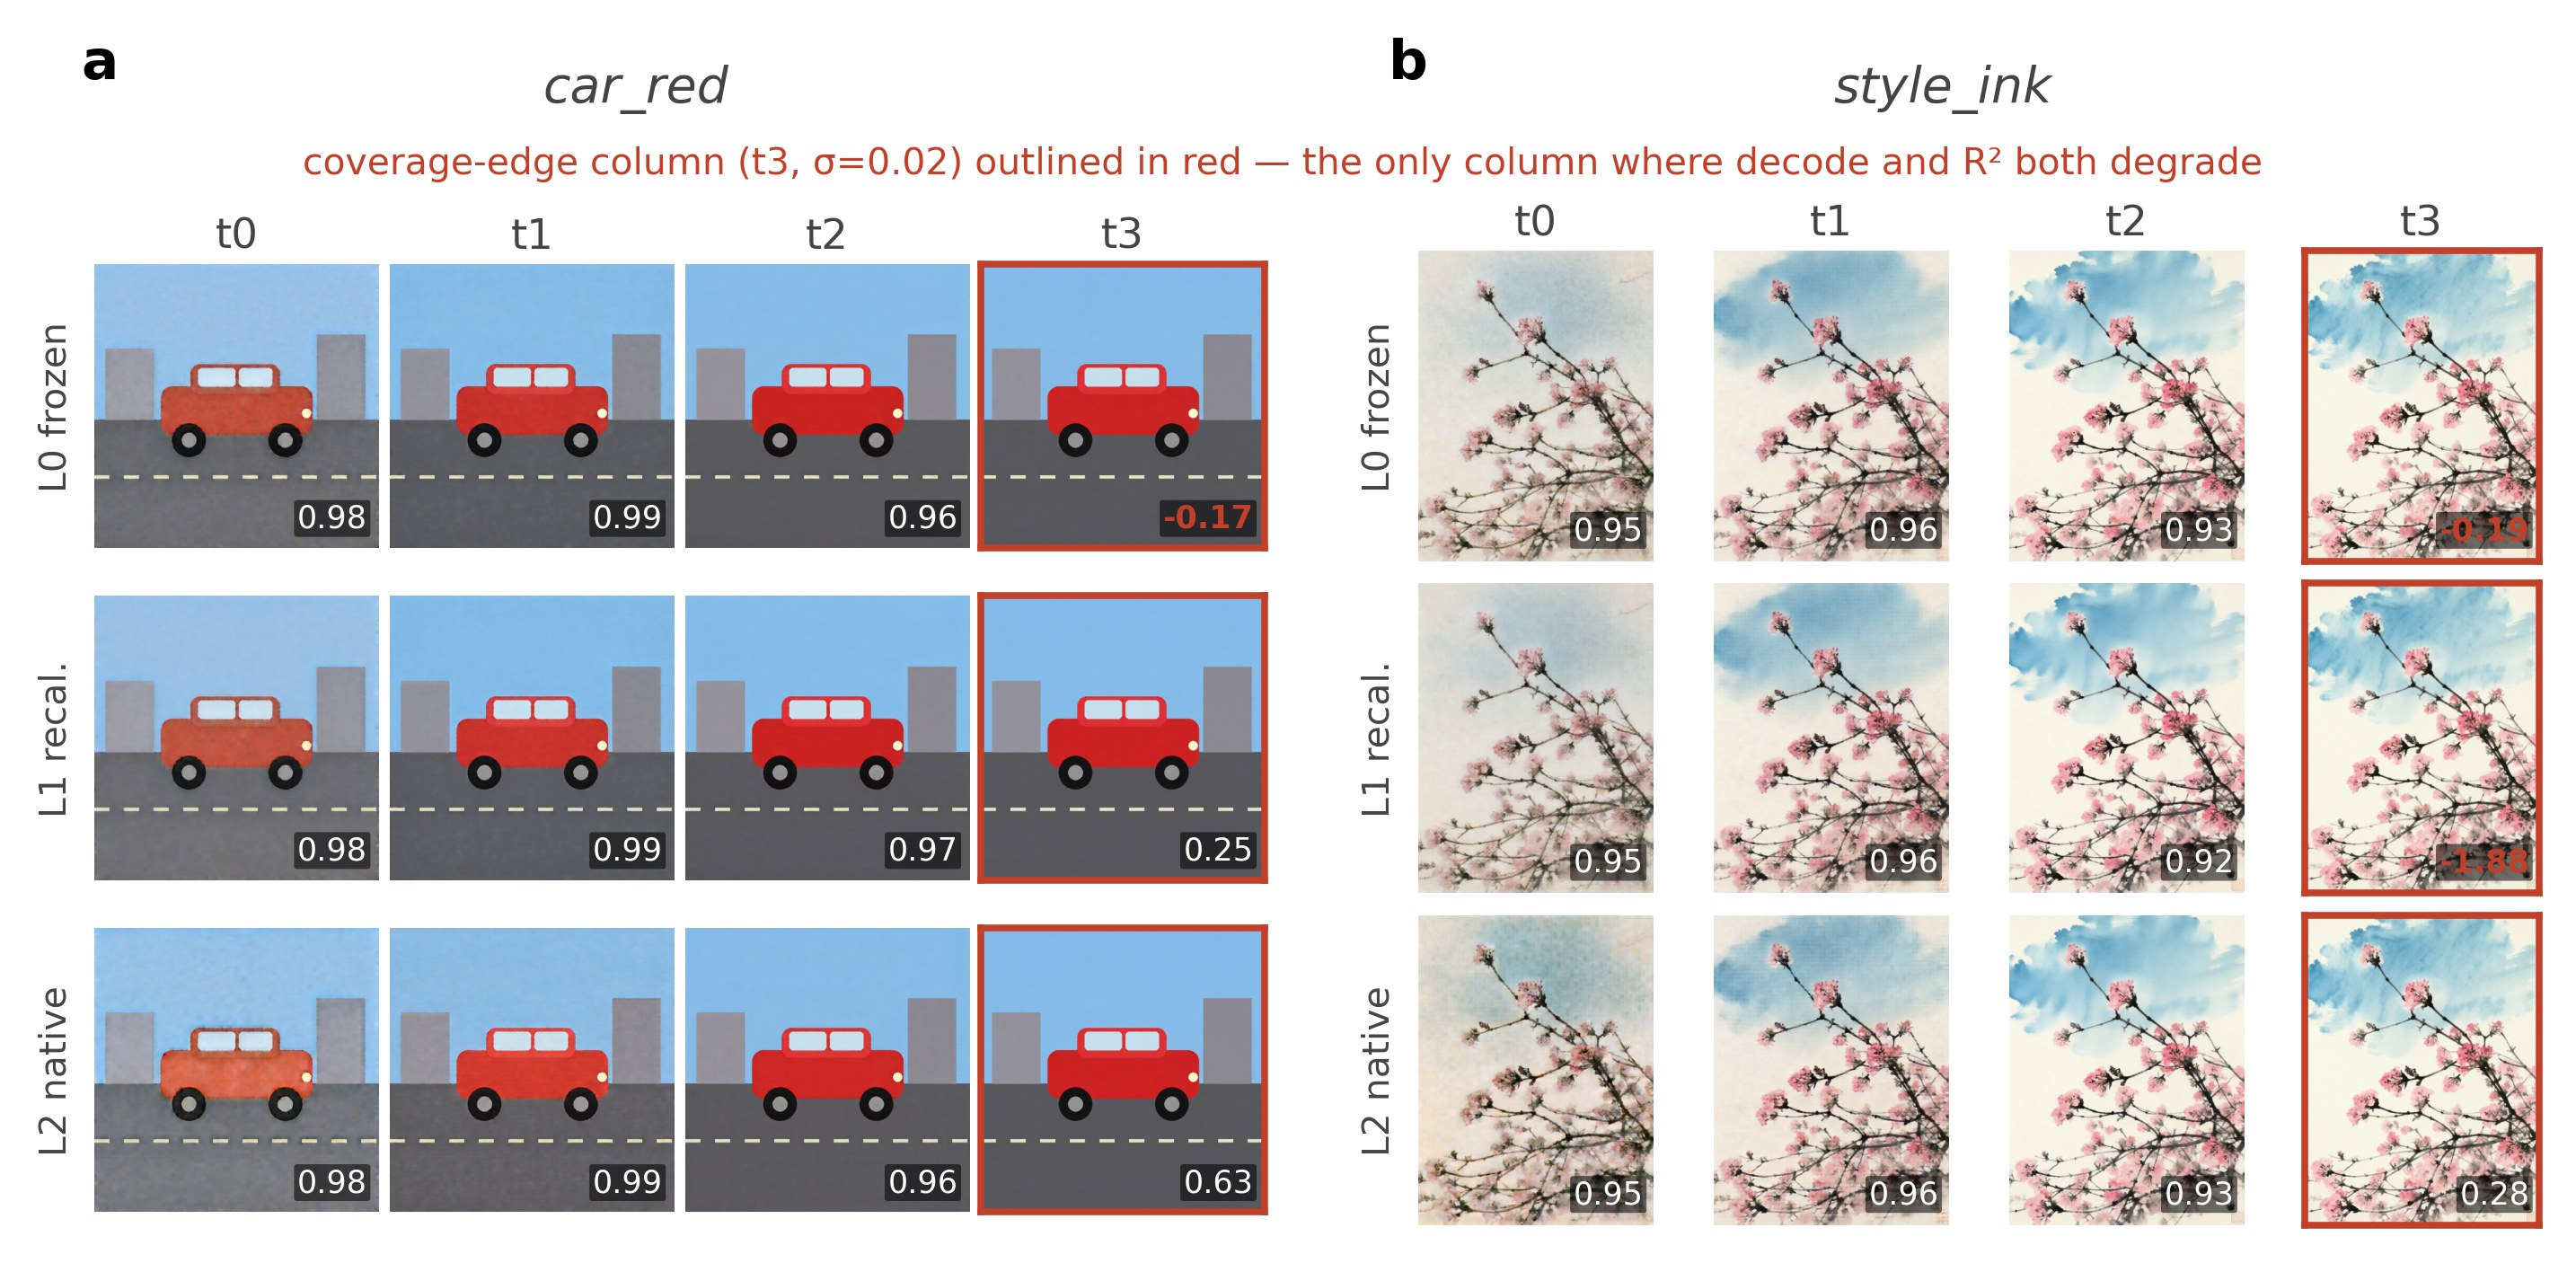
\includegraphics[width=0.98\textwidth]{figs/fig17_k7_ladder/fig17_k7_ladder.jpg}
  \caption{\textbf{Rapid-AIO L52 decode ladder under the $\sigma$-matched
  three-rung translator dictionary (K7).} Rows: L0 frozen \model{}
  dictionary, L1 recalibrated, L2 Rapid-AIO-native refit. Columns:
  Rapid-AIO's four sampling steps $t{=}0$--$3$. \textbf{(a)}
  \emph{car\_red}. \textbf{(b)} \emph{style\_ink}. Per-cell numbers are
  the held-out velocity-space $R^2$ for that rung/step. Decode quality
  visibly degrades only in the coverage-edge final column
  ($\sigma{=}0.02$, red outline); the $R^2$ there is negative for
  \emph{style\_ink} L1 even though the pixel decode is a clean ink
  painting, the pixel-invisible failure mode described in prose. Data:
  \texttt{runs/k7\_rapid\_ladder/}.}
  \label{fig:k7ladder}
\end{figure*}

\textbf{Decomposing the terminal-step collapse: coverage versus
intrinsic decodability.} Is the negative terminal-step $R^2$ above a
missing dictionary entry, or a genuine loss of linear decodability? A
follow-up two-phase check (K8) captures three more \model{} dictionary
entries at $\sigma=0.20, 0.11, 0.02$ and separately re-fits \model{}'s
own held-out native ridge at those same steps (zero cross-model
shift). The two causes dissociate cleanly and the data force the
dissociation: as the borrowed $\sigma$ closes in on Rapid-AIO's
terminal $\sigma=0.02$, zero-shot transfer rises monotonically from
negative toward the native ceiling on 5/6 deep curves (\emph{car\_red}'s
three deep layers land within $0.013$--$0.133$ of it) -- the
$\sigma$-keying law holds all the way to the terminal step, and K7's
negative numbers were a hole in the captured grid, not a
terminal-step transfer breakdown. Independently, \model{}'s own
native held-out fit collapses at the same step for the same mid-deep
layer (L52: \emph{car\_red} $0.98\to0.66$, \emph{style\_ink}
$0.96\to0.29$; L56 also drops, to $0.774$ for \emph{car\_red}) while
L59 stays at $0.99$ -- a model-independent loss of decodability, not
a transfer artifact. Recovery is partial, not uniformly at parity:
even $\sigma$-matched, \emph{car\_red} L52 reaches only $0.49$ against
a $0.63$ native ceiling. L59's perfect score is close to tautological
-- it feeds the velocity head directly and is decodable from any
step's data -- so it is the control that makes the L52/L56 drop
legible, not a finding in its own right. The cleanest single result:
K7's ``recalibration backfires'' anomaly (\emph{style\_ink} L1 at the
terminal step: $-1.88$) was entirely a wrong-$\sigma$-weight artifact
-- recalibrating with the correctly-matched $\sigma=0.02$ weight
instead recovers gains at all six deep cells, reinforcing rather than
contradicting the $\sigma$-keying account. Left open: whether the
terminal-step collapse reflects genuine nonlinearity or the limited
capacity of a three-case ridge fit -- both native fits share that
limitation, so this axis is untouched by the above; the same fit
stays healthy at the three preceding steps and drops only at the
terminal one, a step-specific pattern that favors nonlinearity over
capacity without settling it.

\begin{figure*}[t]
  \centering
  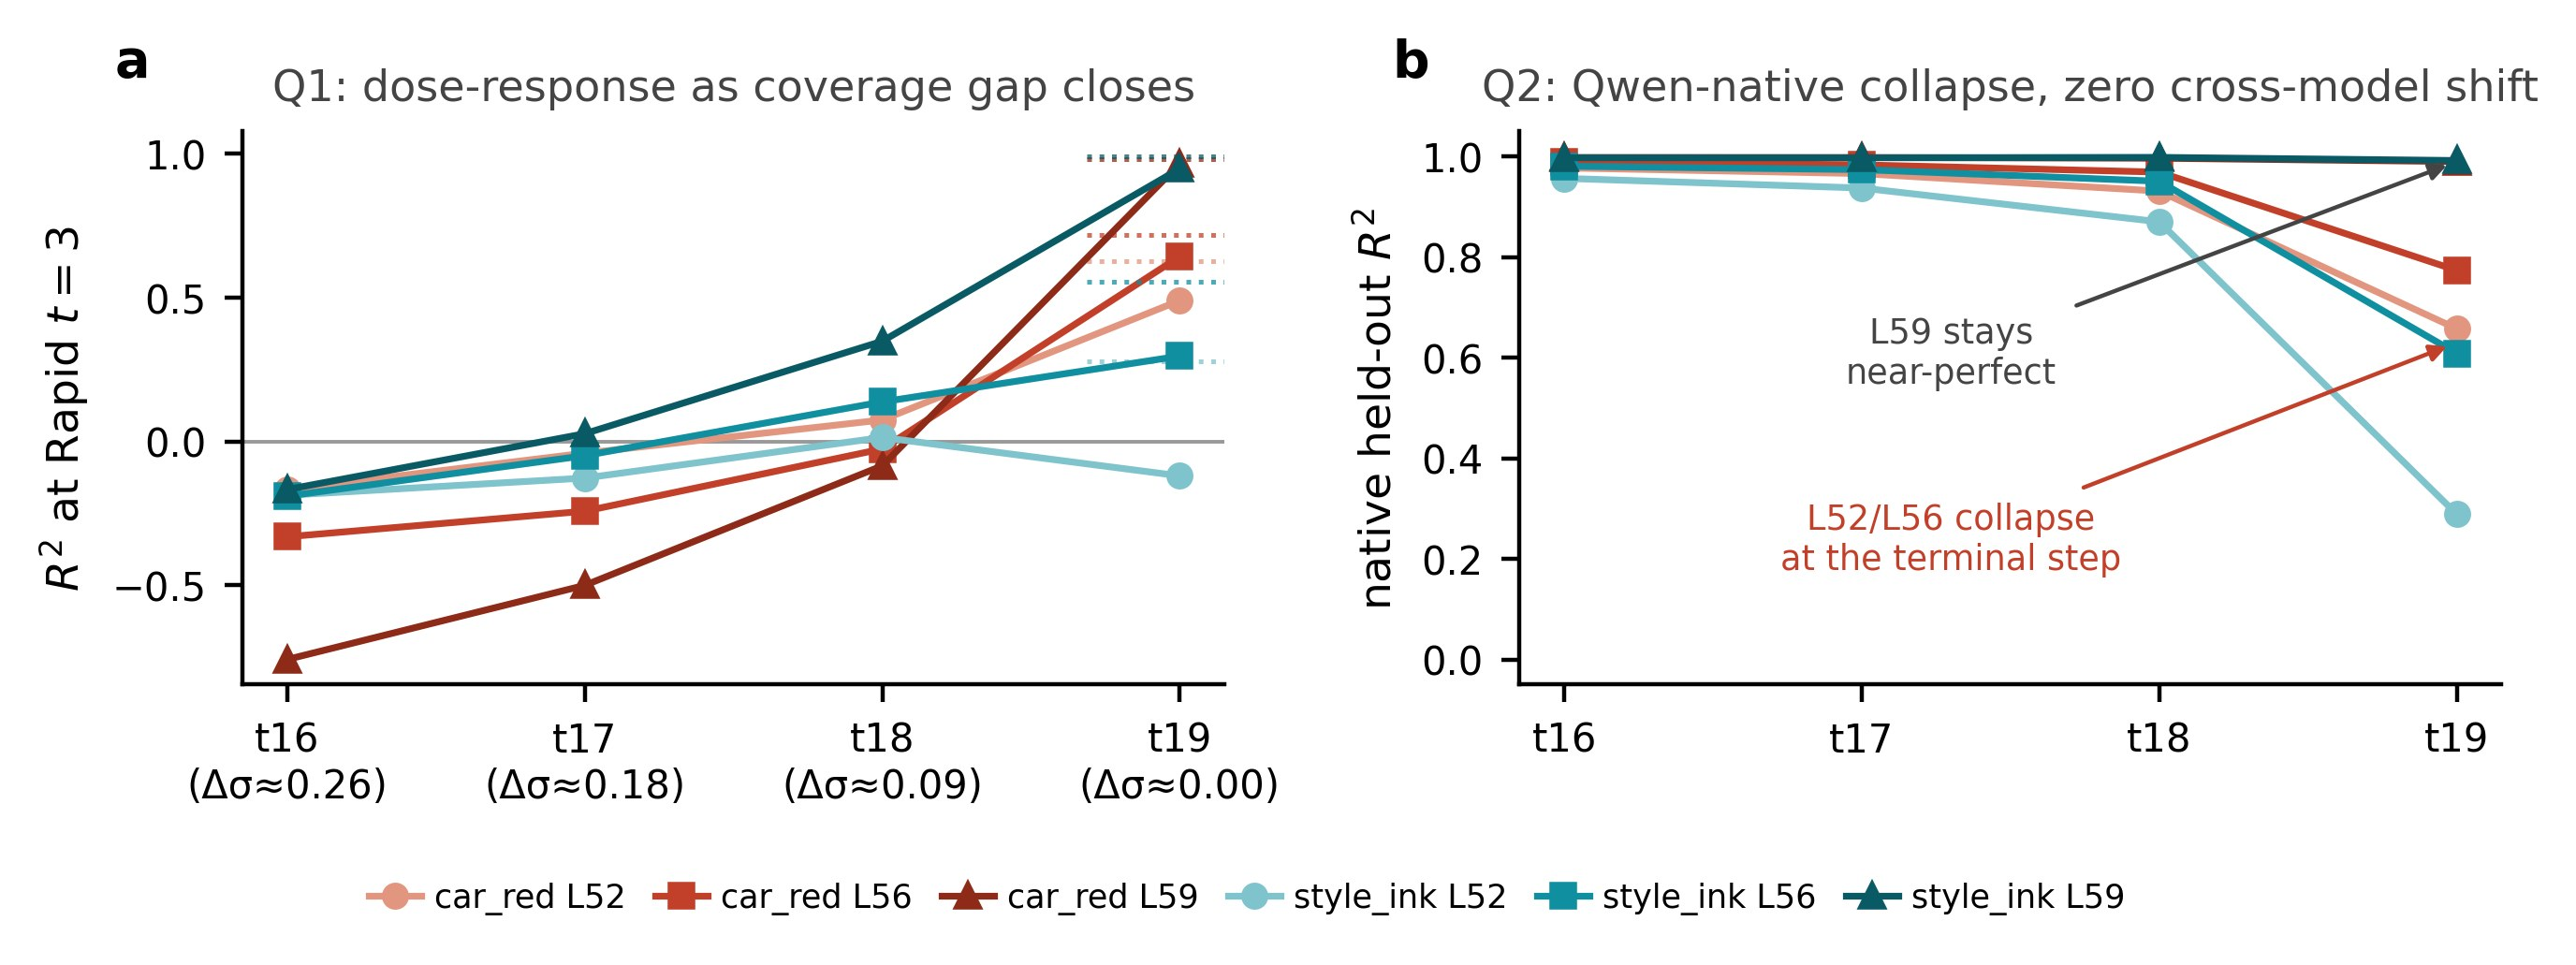
\includegraphics[width=0.98\textwidth]{figs/fig18_k8_decompose/fig18_k8_decompose.jpg}
  \caption{\textbf{Decomposing K7's terminal-step collapse into
  coverage and intrinsic-decodability causes (K8).} \textbf{(a)} Q1:
  as the borrowed \model{} dictionary entry's $\sigma$ closes in on
  Rapid-AIO's terminal $\sigma{=}0.02$ (left to right), zero-shot
  transfer $R^2$ at Rapid $t{=}3$ rises monotonically toward each
  cell's native-refit ceiling (dotted) on 5/6 deep curves -- a
  coverage gap, not a terminal-step transfer breakdown. \textbf{(b)}
  Q2: \model{}'s own held-out native refit, with zero cross-model
  shift, collapses at the same terminal step for L52/L56 while L59
  stays at $0.99$ -- a model-independent loss of decodability. Data:
  \texttt{runs/k8\_sigma\_coverage/}.}
  \label{fig:k8decompose}
\end{figure*}

\textbf{Closing the axis: a nested learning curve isolates
nonlinearity from fit capacity (K9).} The question K8 left open --
intrinsic nonlinearity or three-case ridge capacity -- is settled by
a nested curve over $N=3,6,9,12$ training cases, read via
train--val fit rather than the held-out curve alone. Train--val
$R^2$ at the terminal step plateaus at $\approx0.80$ for L52
($0.792/0.830/0.808/0.805$ across $N$) and $\approx0.90$ for L56,
invariant to $N$. The linear map cannot fit even its own training
data above this ceiling regardless of data volume -- an expressivity
ceiling, not undersampling, since capacity starvation would instead
push train--val toward $1.0$ as $N$ grows. A real, secondary
small-$N$ gap sits on top: held-out $R^2$ rises $N{=}3\to6$ (L52:
\emph{car\_red} $0.649\to0.759$, \emph{style\_ink}
$0.271\to0.539$) but saturates by $N{=}6$--$9$, converging onto the
train--val ceiling for \emph{car\_red} ($0.785$ vs.\ $0.805$ at
$N{=}12$) while \emph{style\_ink} retains a residual gap ($0.574$
vs.\ $0.805$); a composition swap confirms the rise tracks $N$, not
which cases were added (all diffs $<0.055$). The layer gradient
matches K8: L59 stays linear (train--val $0.998$), L56 a mild
ceiling, L52 the strongest. Three caveats: the ceiling holds for the
\emph{linear-readout} class specifically (ridge on raw hidden
state) -- L52 is not \emph{linearly} decodable above
$\approx0.80$, not undecodable outright, since a nonlinear probe
might recover more; the pre-registered point prediction
($\Delta<0.15$) was refuted ($\Delta=+0.22$, the pre-registered
ambiguous band), so the naive flat-from-$N{=}3$ expectation was too
strong -- only the pre-registered tie-break of reading that band
with train--val resolves it toward nonlinearity; and $N$ is capped
at 12 (all available same-protocol cases), so the train--val plateau
makes $N>12$ unlikely to move the ceiling, but this is an
extrapolation.

\begin{figure*}[t]
  \centering
  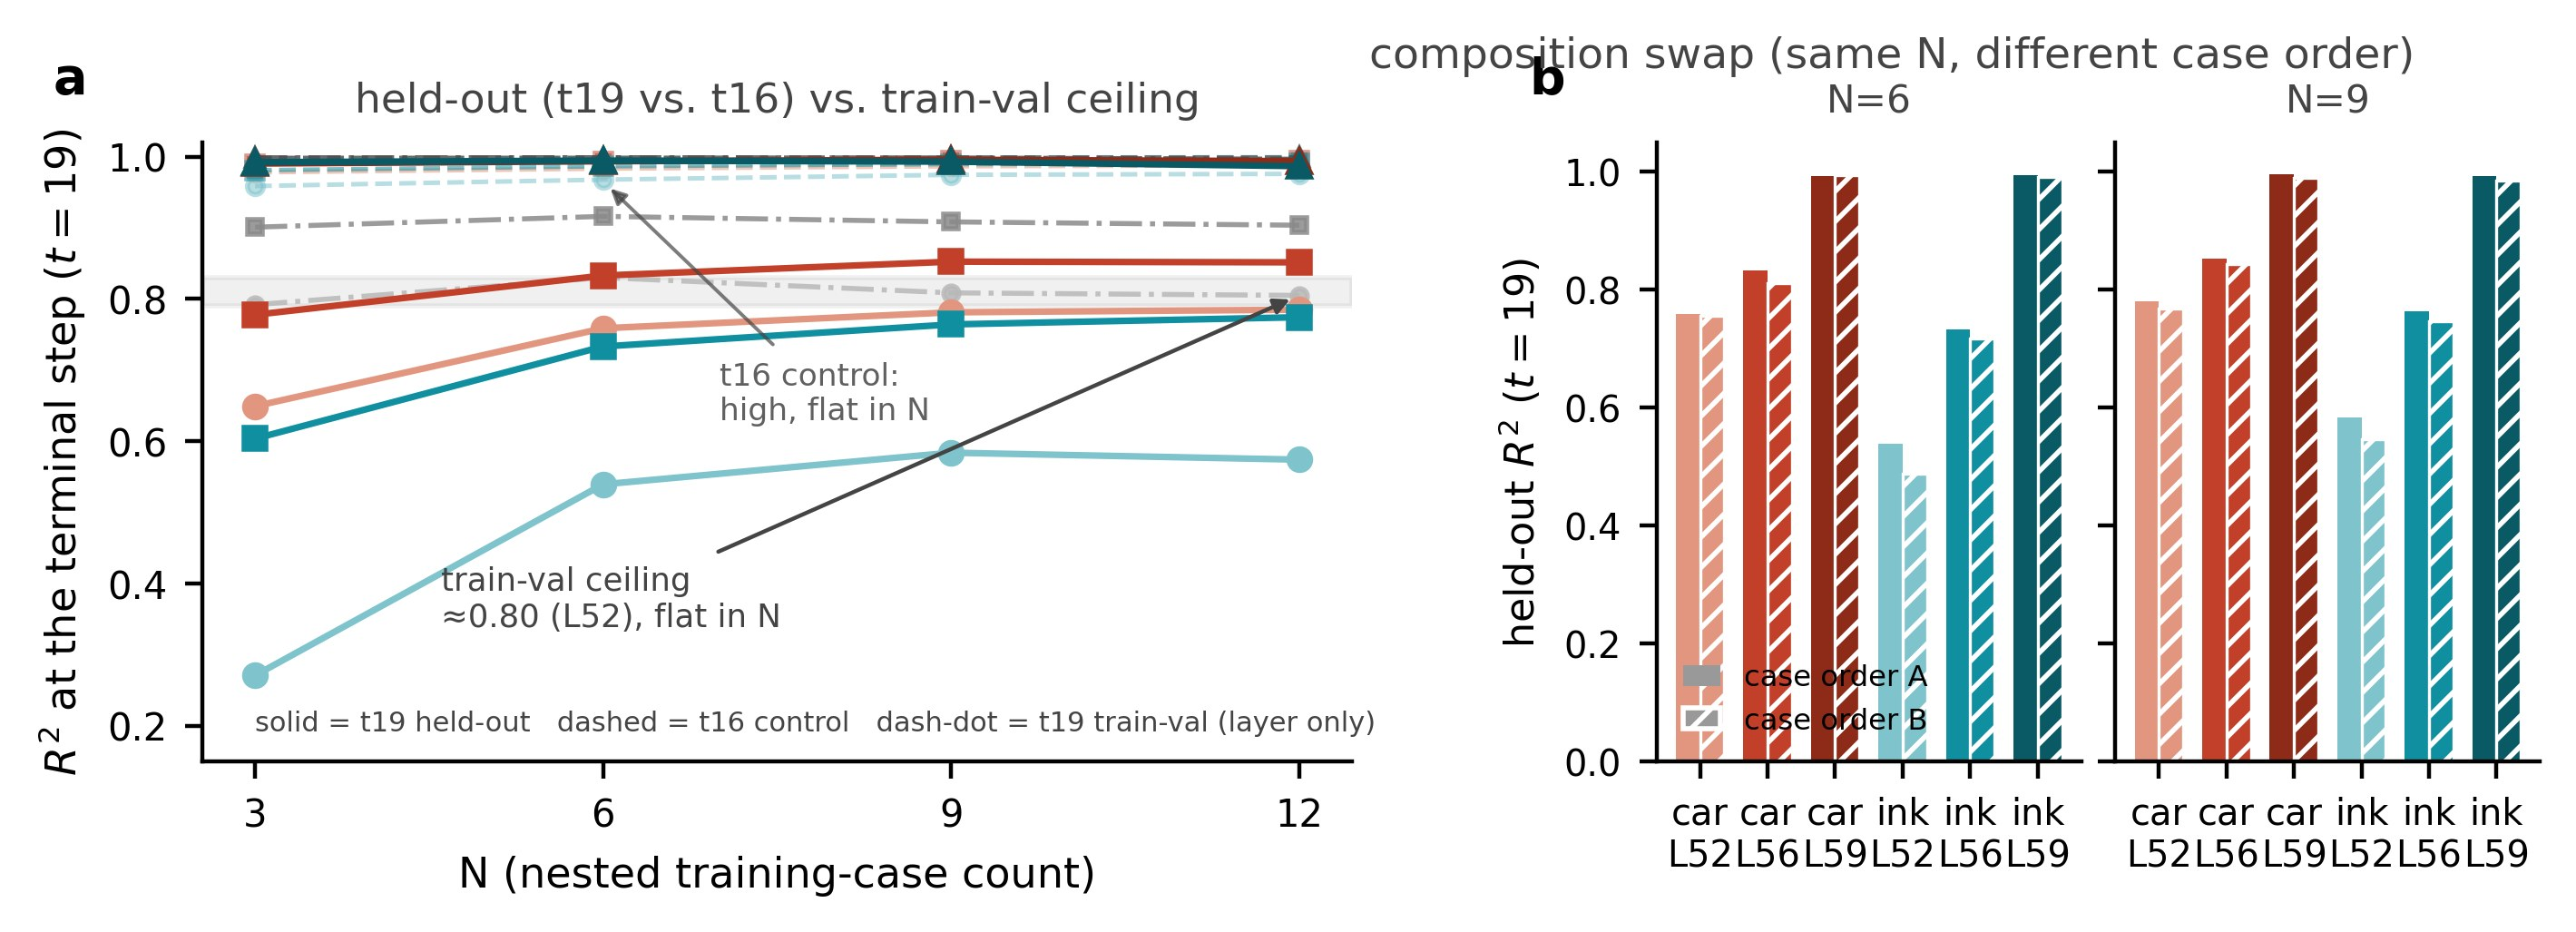
\includegraphics[width=0.98\textwidth]{figs/fig19_k9_curve/fig19_k9_curve.jpg}
  \caption{\textbf{Nested learning curve isolates nonlinearity from
  fit capacity (K9).} \textbf{(a)} Held-out $R^2$ (solid, by
  case$\times$layer) and train--val $R^2$ (dash-dot, layer only) at
  the terminal step ($t{=}19$) vs.\ nested training-case count $N$.
  Train--val plateaus at $\approx0.80$ (L52) / $\approx0.90$ (L56),
  invariant to $N$ -- an expressivity ceiling, not undersampling.
  \textbf{(b)} Composition-swap control: held-out $R^2$ under two
  independent case orderings at matched $N$ (N6 vs.\ N6$'$, N9 vs.\
  N9$'$) agree to within $0.055$, confirming the $N{=}3{\to}6$ rise
  tracks case count, not which cases were added. Data:
  \texttt{runs/k9\_capacity\_curve/}.}
  \label{fig:k9curve}
\end{figure*}

\subsection{Across edit families: a two-axis law and a steerability
spectrum}\label{sec:families}

\begin{figure*}[t]
  \centering
  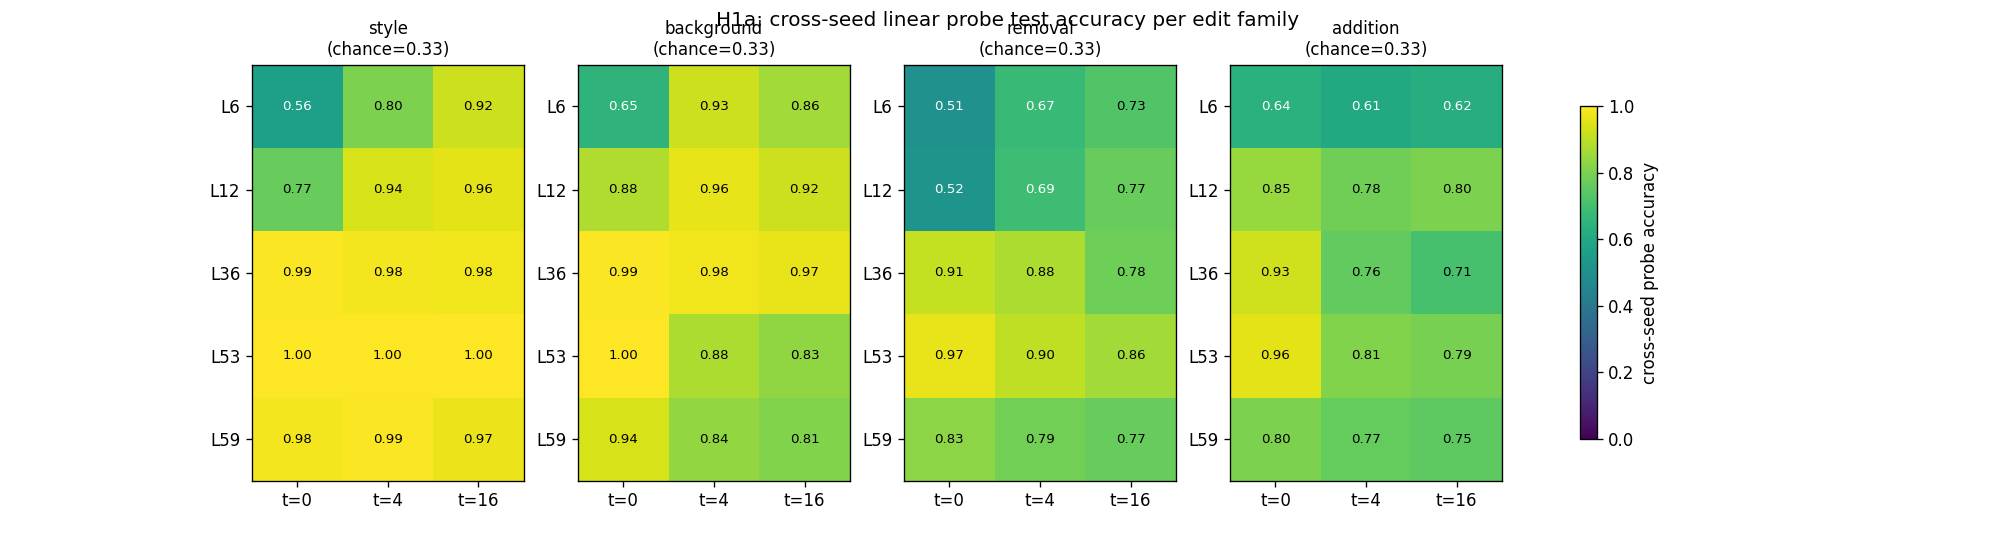
\includegraphics[width=0.98\textwidth]{figs/h1a_family_probes/h1a_family_probes.png}
  \caption{Cross-seed probe accuracy per edit family (chance $=0.33$),
  the identical protocol behind Figure~\ref{fig:mechanism} (right):
  three prompts per family (two real edits plus one neutral), probe
  trained on seed 0 and tested on seed 1, on region-appropriate token
  rows (whole frame for style, background complement of the subject box
  for background, the object box for removal and addition). Appearance
  families (left two) are readable almost immediately in depth;
  structure families (right two) crystallize only mid-stack (removal
  crosses $0.88$ at L36) or never cleanly at $t\ge4$ (addition).}
  \label{fig:families}
\end{figure*}

\begin{figure}[!tp]
  \centering
  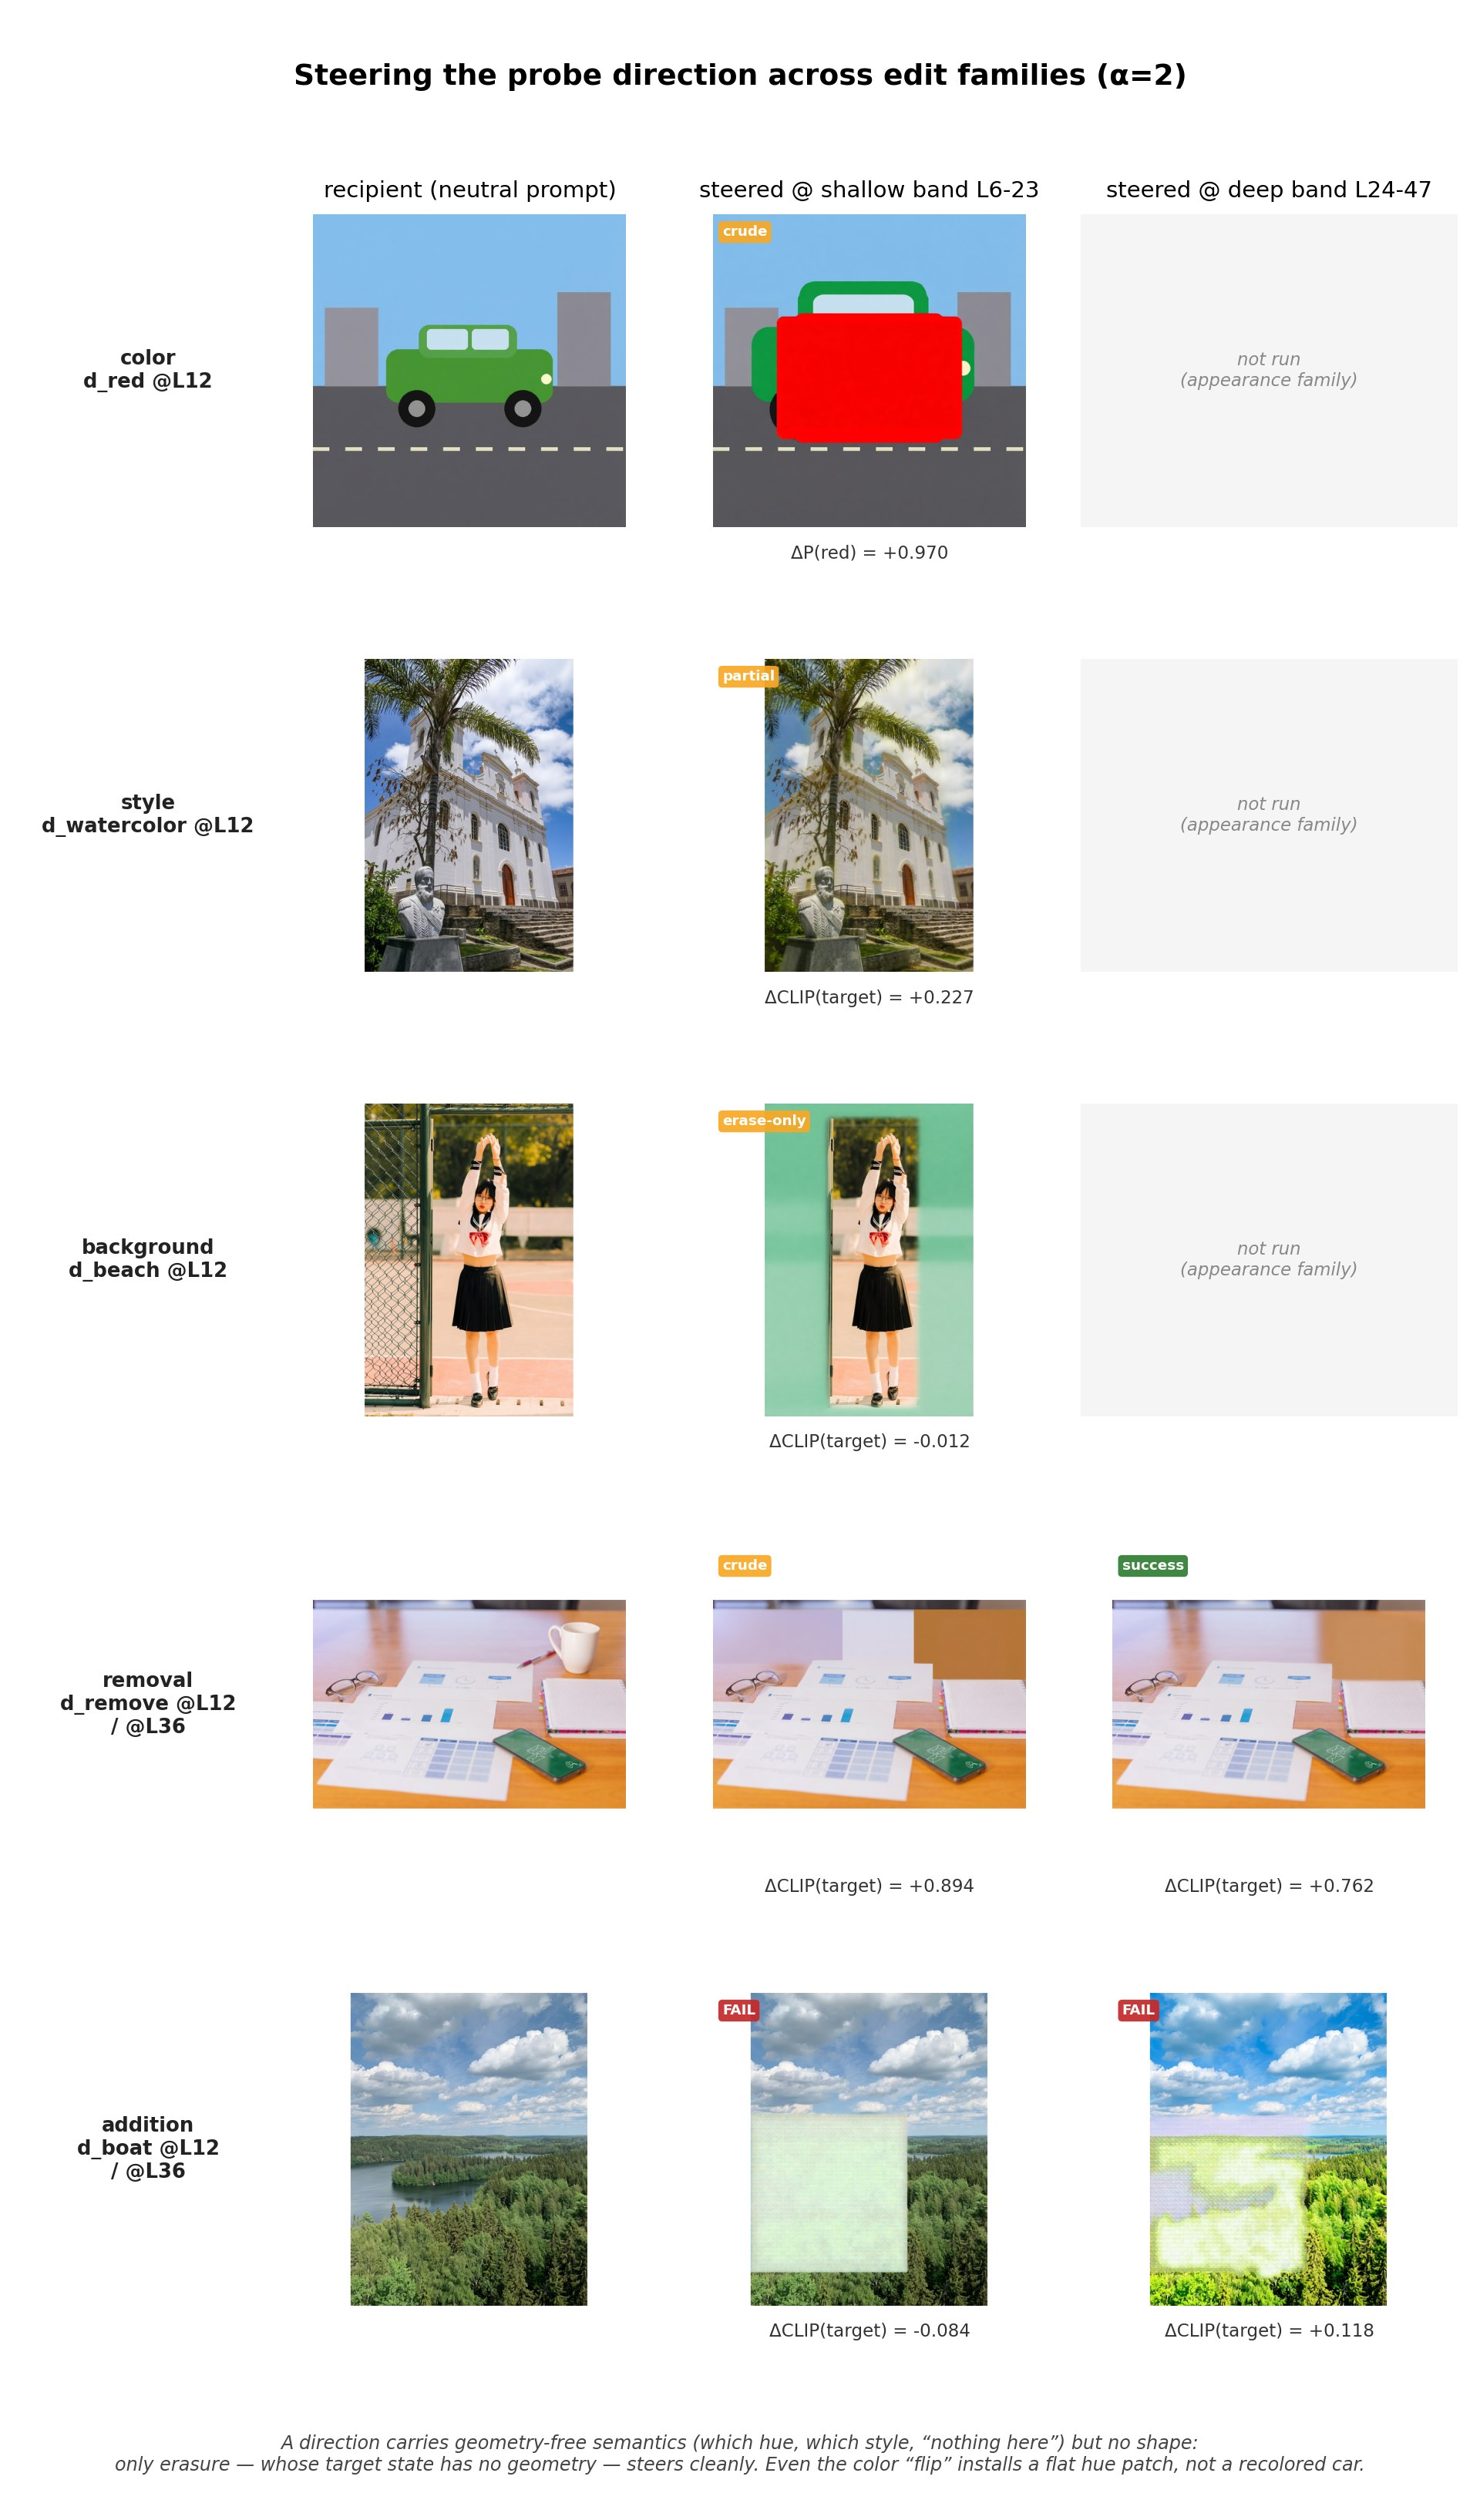
\includegraphics[width=0.88\columnwidth]{figs/h1b_steer_spectrum/h1b_steer_spectrum.jpg}
  \caption{Steering each family's own probe direction ($\alpha{=}2$)
  into a neutral-prompt recipient, at the shallow band L6--23 (middle
  column) and, for the structure families, with a direction re-trained
  at L36 and applied at L24--47 (right column). Verdict badges are from
  visual inspection of every output against its baseline; CLIP gains
  corroborate but do not decide (by CLIP alone the crude L12 removal,
  $+0.89$, would outrank the clean L36 one, $+0.76$). Only removal --
  the one edit whose target state has no geometry -- steers cleanly.}
  \label{fig:steerspectrum}
\end{figure}

Nearly everything above rests most heavily on color edits -- the probe
of \S\ref{sec:mechanism} is literally a three-color classifier. To ask
how much of the picture is about \emph{color} rather than about
\emph{editing}, we re-ran the two core readouts (the A/C decode
crossover and the cross-seed probe grid) and the steering intervention
on four further edit families -- global stylization (watercolor vs.\
pencil sketch vs.\ neutral enhance), background swap (beach vs.\ snowy
forest vs.\ keep), object removal (remove the cup vs.\ recolor it vs.\
keep), and object addition (add a boat vs.\ a swan vs.\ keep) -- with
the identical 3-prompt~$\times$~2-seed protocol on region-appropriate
token rows.

\textbf{The measured translation boundary is stable across tested
families; explicit-prompt readability is not.} Wherever the A/C crossover is cleanly measurable it lands in the
same terminal band as color's L52.7--53.6: style at L53.0/53.1
($t{=}4$/$t{=}16$), background at L52.1 ($t{=}16$; at $t{=}4$ the
standard decode already wins from L48 on). For removal and addition the between-variant CLIP margins are
too small to localize a crossover sharply (the removal-label weakness of
\S\ref{sec:limits} again); their sign patterns are consistent with the
same band (nominal crossings L53.4--55.9), and no family puts a boundary
anywhere else in the stack. Explicit prompt-label readability, by contrast,
splits the families in two (Figure~\ref{fig:families}): the appearance
families are readable shallow -- style $0.80$ at L6/$t$4 and $0.94$ at
L12/$t$4, background $0.93$ and $0.96$ at the same cells, right where
color's $0.883$ sits. The structure families lag well behind: removal
is barely above chance there ($0.67$--$0.69$) and crosses $0.88$ only
at L36, and addition never exceeds $0.81$ anywhere at $t\ge4$.
Combined with \S\ref{sec:when}'s onset finding -- insertion edits are
also the ones with delayed visible onset -- this gives a descriptive
two-axis pattern: appearance prompt labels are shallow-readable, while
structure prompt labels require deeper features and insertions can onset
later in time. This is not evidence of irreversible choice. One honest footnote: the
L59 probe dip \S\ref{sec:mechanism} reported is itself family-dependent
-- pronounced for color ($0.68$--$0.75$), mild for background, absent
for style ($0.97$--$0.99$) -- so ``the last block costs linear
separability'' is a color-typical signature, not a universal one.

\textbf{A steerability spectrum: a direction carries no geometry.}
Steering each family's own L12/$t$4 probe direction into its
neutral-prompt recipient ($\alpha{=}2$, layers 6--23, family region;
Figure~\ref{fig:steerspectrum}) does not reproduce one uniform outcome;
it spreads the families across a spectrum. Stylization moves genuinely
but partially -- a visible painterly wash over the whole frame
($\Delta$CLIP $+0.23$). Background swap achieves exactly half the edit:
the fence-and-court background is wiped to a flat field, but no beach
appears ($-0.01$) -- the erase half without the synthesis half. Removal
by CLIP succeeds ($+0.89$) but crudely, with flat color patches scarring
the region above the desk. Addition destroys its region outright
($-0.08$). Re-training the two structure directions at L36 -- the depth
where removal first becomes readable -- and steering the deep band
L24--47 resolves the split: removal becomes \emph{clean} (the cup
vanishes and the wall behind it is naturally inpainted; $+0.76$, with
off-region damage falling from $5.9$ to $1.9$), while addition still
fails ($+0.12$ is a blob artifact; off-region damage $28.6$). A
same-norm random direction moves nothing ($+0.001$, output visually
identical to the recipient).

Together with \S\ref{sec:steer}'s corrected reading of the color flip,
the spectrum reads as one rule: a stored direction carries
\emph{geometry-free} semantics -- which hue, which style, ``nothing
here'' -- but cannot carry shape. It can suppress or reweight content
that is already present, and it can do so cleanly exactly when the
target state requires no geometry to be specified: erasure steers
cleanly (at the depth where its prompt label becomes readable), a global
style wash steers partially, a recolor-in-place installs the hue but
loses the object (\S\ref{sec:recompose} revisits this case), a
background swap executes only its erasure half, and insertion -- pure
geometry specification -- fails at every depth we tried. Erasure is
linear because emptiness has no shape. This sharpens \S\ref{sec:steer}:
the ``what'' a direction can carry is a suppression/reweighting target
over existing content, not a specification of new structure -- for
that, transplant (\S\ref{sec:swap}), which moves an entire hidden state
rather than one direction, remains the cheapest sufficient intervention
we found. \S\ref{sec:recompose} shows this rule needs one qualification:
what the recolor-in-place direction lost above was not geometry but
\emph{scope} -- confined to the edited object's own silhouette, the same
direction keeps the geometry too.

\FloatBarrier
\subsection{Recomposing edits in place: masks are the carrier}\label{sec:recompose}

\begin{figure}[t]
  \centering
  \begin{subfigure}[b]{0.47\columnwidth}
    \centering
    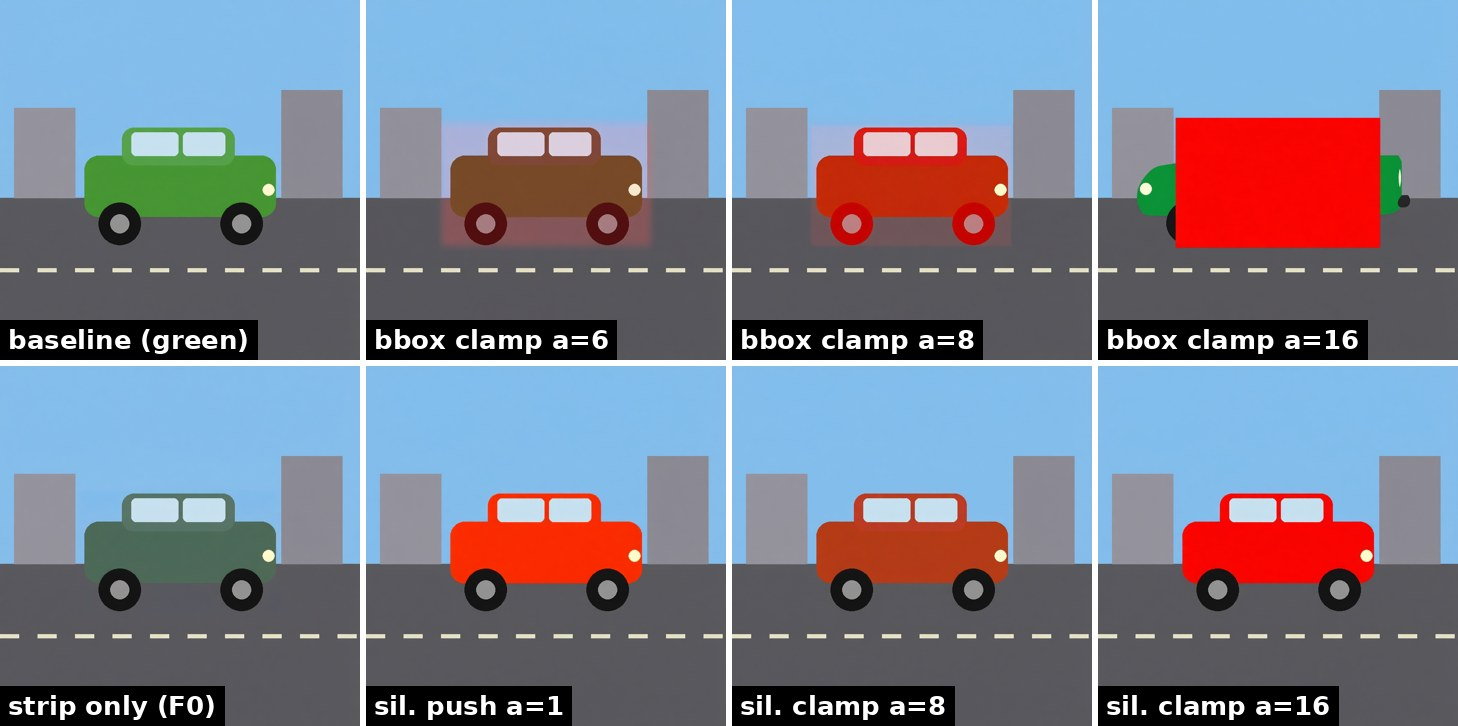
\includegraphics[width=\linewidth]{figs/i1d_recompose_grid/i1d_recompose_grid.jpg}
    \caption{}
    \label{fig:recompose}
  \end{subfigure}
  \hfill
  \begin{subfigure}[b]{0.47\columnwidth}
    \centering
    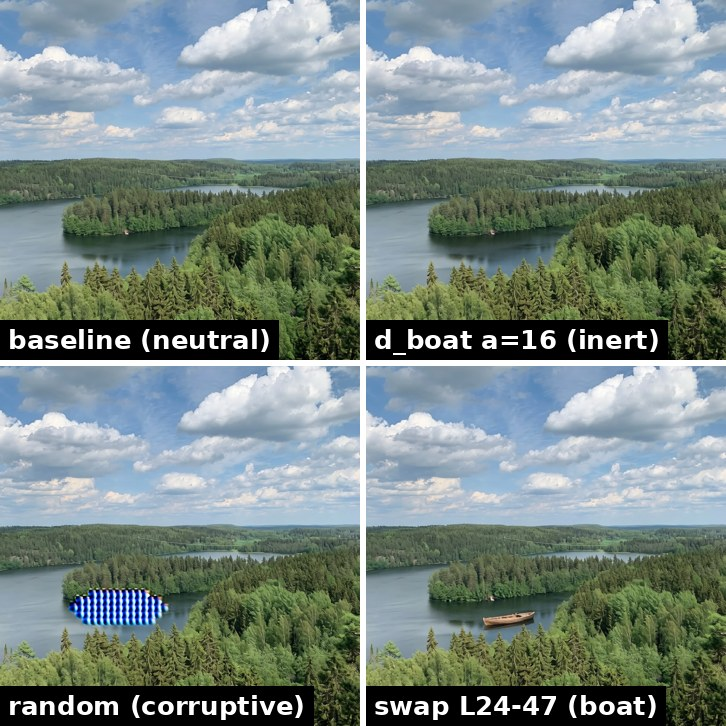
\includegraphics[width=\linewidth]{figs/i2_taxonomy_grid/i2_taxonomy_grid.jpg}
    \caption{}
    \label{fig:taxonomy}
  \end{subfigure}
  \caption{\textbf{(a)} Car dose ladder, bbox vs.\ silhouette mask
  (\S\ref{sec:recompose}). \textbf{(b)} Direction taxonomy on the lake
  hull (\S\ref{sec:recompose}). Data: \texttt{runs/i1\_recompose,
  i1b\_write\_fix,i1c\_dose\_window,i1d\_silhouette} (a);
  \texttt{runs/i2\_mask\_synthesis,i2b\_mask\_synthesis\_deep,
  i2c\_swap\_control} (b); both to be rendered from these runs' outputs.}
  \label{fig:recomposetaxonomy}
\end{figure}

This subsection is where the opening sentence's middle clause --
\emph{bound to a spatial carrier} -- stops being a metaphor.
\S\ref{sec:steer}'s dose-response and \S\ref{sec:families}'s spectrum
both steer a bounding box. Here we ask directly: when a steered color
direction destroys the object it recolors, is the geometry actually
gone, or did we steer the wrong tokens?

\textbf{Erasure is separable at rank 1; writing self-cancels for an
uninteresting reason.} Projecting the \emph{car\_green} recipient's car
rows onto the complement of a QR-derived rank-2 color subspace ($1.2\%$
of row norm on average) desaturates the car from saturated green
($P(\text{green})=0.486$) to sage ($0.327$) with geometry
pixel-identical (in-bbox diff $13.6$, out-of-bbox $0.37$); a single
rank-1 direction alone reproduces almost the same desaturation (diff
$14.9$) -- the color attribute is rank-1, and stripping it costs nothing
else. Pushing a new color \emph{into} the stripped rows first failed
because re-projecting at each of 18 steered layers strips the previous
layer's own addition before the next can add to it, so the accumulated
push never reddens the car -- a write-side bug we flag once rather than
re-derive.

\textbf{Clamp semantics recover a clean write, inside a narrow,
direction-dependent dose window.} Projecting out the old color and
writing the new target coordinate independently at every layer
(``clamp'') breaks the self-cancellation: at $\alpha{=}8$ the car turns
clean red, geometry intact, with only a faint haze over the rest of the
region -- the first clean in-place attribute rewrite in the project
($P(\text{red})=0.091$; CLIP badly \emph{under}-scores this, since the
haze pulls the label from ``red car'' even though open-set mass is
$0.907$). The identical accumulated push at matched $\alpha{=}8$ floods
the box instead (fidelity outside $33.4$ vs.\ clamp's $1.4$), confirming
the push itself overwhelms the region. Sweeping $\alpha$ under clamp
traces a continuous hue dial: $\alpha{=}4$ erase-only, $\alpha{=}6$ a
brown blend with geometry intact, $\alpha{=}8$ clean red, and
$\alpha{\ge}10$ a flat bbox-shaped patch ($P(\text{red})=0.70$--$0.84$,
inverting visual truth against the real car's $0.091$); the same
$\alpha{=}8$ reversed (red$\to$green) lands only mid-transition.

\textbf{The overshoot is object-membership recruitment, not carrier
destruction -- and the fix is a mask.} The $\alpha{\ge}10$ patch is
\emph{exactly} bbox-shaped, suggesting the write recruits every steered
token, sky and road included, into ``this is red car body.'' Confining
the identical intervention -- any dose from $\alpha{=}1$ push through
$\alpha{=}16$ clamp -- to the car's own silhouette (371 of 792 in-bbox
patches) turns every one into a perfect recolor: original windows,
wheels, and headlight, no halo, rest of scene untouched (out-of-bbox
diff $0.46$--$0.57$). The same $\alpha{=}16$ that gave a flat rectangle
under the bbox mask gives a clean car under the silhouette. CLIP still
under-scores all four ($0.16$--$0.64$). We read this as a fourth
correction to a reading we had stated with increasing confidence across
\S\ref{sec:steer} and \S\ref{sec:families}: what looked like a
direction's inability to carry shape was our own choice of \emph{where}
to apply it. The carrier is the spatial support you steer -- supply the
object's own mask and the direction does the rest.

\begin{table}[t]
\centering
\footnotesize
\setlength{\tabcolsep}{3.5pt}
\begin{tabular}{@{}llc@{}}
\toprule
Direction & Site & Outcome \\
\midrule
Attribute (color) & silhouette & executable \\
Probe dir.\ (boat/swan) & hull, both depths & inert \\
Random dir.\ (control) & hull, both depths & corruptive \\
Diff modes, rank 1 & hull, deep & category, incoherent \\
Diff modes, rank 4 & hull, deep & instance, wrong id. \\
Diff modes, rank 16 & hull, deep & right material \\
Diff modes, rank 64 & hull, deep & faithful \\
Full nonlinear (swap) & hull, deep & sufficient \\
Jacobian, top-16 & hull, deep & dark blob, non-semantic \\
\bottomrule
\end{tabular}
\caption{Interventions on a spatial mask a linear probe direction
could not fill with a boat. The rank ladder (middle rows) writes only
the donor$-$recipient difference's top-$k$ singular subspace,
$h \leftarrow h + QQ^{\top}(h_{\text{donor}}-h)$, resolving ``only the
full donor state succeeds'' into graded semantic shells. Attribute row
is the car-silhouette result above; all others share one 61-patch lake
hull. The Jacobian row is a donor-\emph{free} local-gradient basis
(\S\ref{sec:recompose}), included for contrast with the rank ladder's
donor-dependent write basis. Data: \texttt{runs/i2\_mask\_synthesis},
\texttt{i2b\_mask\_synthesis\_deep}, \texttt{i2c\_swap\_control},
\texttt{j1\_rank\_ladder}, \texttt{k2\_jacobian\_lens}.}
\label{tab:taxonomy}
\end{table}

\textbf{A direction that can recolor an object cannot conjure one, at
any depth: object identity is a nonlinear code.} If mask choice was the
whole story, a mask should also rescue addition's steering failure
(\S\ref{sec:families}). It does not. Steering the same 61-patch hull
mask on the empty lake with the family's own boat/swan probe direction
-- shallow L6--23, every semantics and dose tried, and again re-trained
at L36 and applied at the deep L24--47 band where addition semantics
actually crystallizes -- is visually indistinguishable from doing
nothing (diff $2.4$--$7.5$ at both depths, including the $\alpha{=}16$
dose that fully recolors the car). A same-norm random direction in the
identical mask is not inert: it renders a corrupted, mask-shaped blob
(diff $51$--$87$), confirming the mask can carry something and the
boat/swan directions are specifically computed away downstream, not
merely too weak. Only transplanting a donor's actual (nonlinear,
high-rank) hidden state into the same 61 tokens -- not its linear probe
projection -- grows a real boat, and only from the deep band (L24--47
clean; L0--23 only a faint ghost) -- a third confirmation,
after probe accuracy and steering depth (\S\ref{sec:families}), of the
same depth split, now at the level of what a swap can carry.
Table~\ref{tab:taxonomy}/Figure~\ref{fig:taxonomy} summarize the
complete four-way taxonomy. Object information is token-local -- 61
rows suffice -- but lives in a code a rank-1 write cannot reconstruct:
linear readability and linear writability are not the same property, and
which one a variable has depends on its kind -- an existing object's
attribute is writable, a not-yet-existing object's identity is readable
but not writable at rank 1.

\textbf{A rank ladder dissolves ``nonlinear'' into graded semantic
shells -- and separates the read basis from the write basis.} The
taxonomy's inert row used \emph{probe} directions: the basis in which
object identity is easiest to \emph{read}. Replacing them with the
basis in which the state actually \emph{changes} -- per-layer top-$k$
right singular vectors of the donor$-$recipient difference on the same
61 tokens (L24--47) -- and writing only that subspace's component,
$h \leftarrow h + QQ^{\top}(h_{\text{donor}} - h)$, turns the binary
(inert vs.\ full swap) into a ladder with visible semantic shells.
Rank 1 ($36.5\%$ of difference energy) evokes the \emph{category} but
no instance -- an incoherent flotilla of boat-fragments, emphatically
not inert, unlike the probe direction on the identical mask; rank 4
yields a single coherent vessel of the wrong identity (a gray
steamer); rank 16 gets the material right (a wooden barge); rank 64 --
$2\%$ of the model dimension, $89\%$ of the difference energy --
reproduces the donor's boat faithfully, visually matching the full
swap. A random 64-dim basis is a null: it captures only ${\sim}2\%$ of
the difference energy under this write rule -- itself a methodological
caution, since projected-swap random controls are self-attenuating
(unlike the fixed-norm random \emph{direction} above, which corrupts).
Region CLIP scored the rank-1 wreckage $P(\text{boat}){=}0.985$, a
fifth documented failure-mode instance: it cannot tell boat-shaped
chaos from a boat. Three revisions follow. Object identity is not a
monolithic nonlinear code: it is linearly writable at modest rank,
coarse-to-fine (category $\to$ instance coherence $\to$ material $\to$
identity). ``Inert'' was a property of the classifier direction, not
of rank-1 writes: the subspace a variable is best \emph{read} from and
the subspace you must \emph{write} to change it are different. And
practically, a donor edit can be stamped from a $48\times$-compressed
bank (store $Q^{\top}h$, 64 dims per token), with $k$ itself a
reference-faithfulness dial.

\textbf{A third basis: local gradients are not the write basis
either.} The rank-ladder write basis above is donor-\emph{dependent}:
it needs a donor state to difference against. A natural donor-free
candidate is the local Jacobian: differentiate a scalar that projects
the network's predicted velocity onto the donor direction, $J =
\sum_v\langle v, a_v\rangle$, back through the block-$\ell$ input (a
leaf-graft-and-checkpoint construction whose gate is bit-exact,
$\max|\text{diff}|=0$), and take the top-16 right singular vectors
$Q_{\text{jac}}$ of that gradient as a local-gradient basis
(\texttt{runs/k2\_jacobian\_lens}). Three pre-registered predictions
are refuted. $Q_{\text{jac}}$ only weakly resembles the rank-ladder
write basis: mean subspace overlap $0.058$ (individual layers
$0.031$--$0.113$) against a random-projection control of $0.0054$ --
$6$--$23\times$ random, but far short of the $0.30$ we required -- and
systematically about twice as large at $t{=}4$ as at $t{=}0$. The
local geometry is itself step-dependent: overlap between the $t{=}0$
and $t{=}4$ Jacobian bases is only $0.15$ ($\sim$30$\times$ random,
but well under the $0.5$ stability line we set). And steering along
$Q_{\text{jac}}$ writes a large amount into the hull (in-hull fidelity
$25.7$--$26.2$ vs.\ the probe direction's $7.2$) but produces no
boat-category evidence at all -- only a dark, non-semantic textured
blob or ink-stain. One prediction is confirmed cleanly: the probe's
read direction $d_{\text{boat}}$ has energy $0.0052$ in
$Q_{\text{jac}}$, matching the random-subspace energy baseline of
$0.0052$ to two decimals -- the read basis is causally orthogonal even
to this local-gradient basis, a third subspace, not only to the
donor-diff write basis. Three bases, three different subspaces: what
is easiest to \emph{read} (the probe), what \emph{changes the state}
when written along (the donor-diff modes), and what is
\emph{locally steepest} toward the donor target (the Jacobian) do not
coincide. The lesson replays adversarial examples inside a generative
model's own latent space: the first-order steepest-ascent direction
toward a semantic target is a shortcut, not semantics. A na\"ive
transplant of the (interpretability-literature) Jacobian-lens idea to
finding a generative write basis does not work; donor differences
remain the gold standard. \emph{Caveat:} gradients are computed in
bf16 (raw norms $\sim10^{-7}$), which may cap the measurable overlap
from below rather than reflect a true ceiling; a path-integrated
Jacobian variant (accumulated across steps rather than a single local
linearization) is untested.

\subsection{A mechanism-derived free lunch: truncating classifier-free
guidance}\label{sec:cfgfreelunch}

Everything above intervenes on the image-stream residual. True CFG
(\S\ref{sec:prelim}) already runs two full forward passes -- conditional
and unconditional -- at every one of the 20 steps. The layer--time map
motivates a direct existence test of whether both passes are needed for
the full trajectory. We run the unconditional pass
only for the first \texttt{cfg\_until} steps and the conditional pass
alone thereafter, on four cases spanning our edit families (recolor,
removal, background swap, addition), against each case's own full-CFG
reference.

\textbf{\texttt{cfg\_until=2} is free.} All four families are visually
intact at \texttt{cfg\_until=2} -- a $45\%$ reduction in forward passes
($22$ of $40$) -- with only ordinary scene variation, not damage, in the
pixel diff (color\_car: $19.3$s$\to$$11.3$s wall time, a $42\%$ measured
saving; background swap keeps its fence-removal and person intact
despite a larger diff of $13.9$ from layout variation). A shallower cut,
\texttt{cfg\_until=4} ($40\%$ fewer passes, $19.3$s$\to$$11.4$s on the
same case), is intact too, with one caveat: \emph{add\_boat} keeps its
edit but drifts in invented-object identity (a longer, flatter barge
instead of the reference's small rowboat) -- late CFG's one visible job
here is stabilizing \emph{what} gets invented, not \emph{whether}.

\textbf{Dropping CFG to zero isolates a tested role in scope.} At \texttt{cfg\_until=0} (zero unconditional forwards, a
measured $2.0\times$ speedup: $9.7$s vs.\ $19.3$s) recolor, removal, and
addition all still land -- the conditional pass alone renders these
three, addition coming out smaller but present. Background
swap half-fails: the beach synthesizes behind the scene, but the
original wire fence and gate are not erased, so the model composites a
new background \emph{around} old structure instead of replacing it
($P(\text{beach})=0.45$, down from $\ge0.996$ at \texttt{cfg\_until}
$\ge2$) -- the mirror image of \S\ref{sec:families}'s steering result on
the same edit (a probe direction erases without synthesizing; a
CFG-free pass synthesizes without erasing). In these cases, CFG's
non-redundant contribution is consistent with resolving \emph{scope}:
deciding which
un-mentioned source content belongs to ``the background'' and must be
suppressed. A twenty-case battery (the full saturation-time battery of
Table~\ref{tab:battery} plus its ten-case extension, spanning color,
removal, background, style, and addition) confirms the recipe: at \texttt{cfg\_until=2}
all 20 edits remain visually intact (mean measured speedup
$1.77\times$), with per-family pixel deviation ordered as the
saturation-time diagnostic predicts (style 7.8--18.0, background 6.0--13.9,
addition $\le$5.4, removal $\le$3.5, color $\le$1.6 mean absolute
pixel difference vs.\ full CFG); the worst visible cost is a mild
softening of one stylization case.

A complementary distillation probe supports the same reading of what the
schedule carries. Running the identical twenty-case battery through a
4-step step-distilled variant of the same architecture (Rapid-AIO v23,
$\sim$2.5s per edit, $7.7\times$ over the 20-step teacher), we
pre-registered that failures should concentrate on delayed-onset,
new-carrier edits (addition first) -- and the prediction was refuted in
the favorable direction: all twenty edits, including every addition
case, land under visual inspection, with only object-identity and
color-grading drift. Together with the boundary-preservation result of
the cross-model section, this suggests step distillation compresses the
sampling \emph{trajectory} while preserving successful edits in this
battery; it does not establish that the same internal computation is
preserved by the $20\!\to\!4$ compression.
(Data: \texttt{runs/x2\_distill\_battery}, single seed, vendor
ancestral-beta sampler with per-case seeding.)

\section{Limitations and Honest Interpretation}\label{sec:limits}

This tool is exploratory and makes no claim about "intent" or
"understanding" in any human sense. Most mechanistic grids use one
model, one or two seeds, and a double-digit count of hand-chosen images.
The fixed-prompt outcome studies are larger but narrow: 48 training
generations per source/model and 12 held-out five-seed groups per
selector. Qwen has two source/prompt selection tasks; Boogu has one.
\S\ref{sec:generalize}'s cross-model replication checks two further
checkpoints on a handful of the paper's headline measurements, not the
full battery, and both are built on \model{}'s own transformer classes --
a fine-tune and a distillation of the same lineage, not an independent
architecture for the full mechanism; Boogu is independent but tests only
early hue prediction and selection. The edit-family sweep (\S\ref{sec:families}) likewise
covers five families but with a single hand-chosen source image per
family. The mask-recomposition study and direction taxonomy
(\S\ref{sec:recompose}) narrow this further still: they run on two
source images (the car, the lake) and one edit each, and the
silhouette/hull masks themselves come from a source-vs-edit pixel diff
or a hand-drawn polygon, not from any segmentation model -- we do not
know whether an automatically-produced mask, a different object shape,
or a different source scene would reproduce the same clean
recolor-at-any-dose result. We do not know how any of these findings
change with model scale, training data outside this lineage, or a
different flow-matching schedule. What follows is a deliberately un-generous accounting of where
the tool itself is unreliable, separate from the open question of
external validity.

\paragraph{CLIP readouts are unreliable in specific, identifiable ways.}
Four failure modes recur throughout this paper. (i) \emph{Removal
labels}: "an empty desk with no cup" is not a well-formed CLIP category
the way "a red car" is, and the object-removal cases in our battery
(\S\ref{sec:when}) show flat, noisy scores that do not track the true
(visually successful) edit outcome at all -- we exclude them from
Figure~\ref{fig:commit} rather than let a broken metric imply a broken
edit. (ii) \emph{Decode-incoherence artifacts}: CLIP will confidently
label pure sampling noise if the label happens to resemble a plausible
texture -- our clearest example is L54/$t$0 of \emph{beach\_background},
still visually noise, scored $P(\text{beach})=0.795$, higher than the
correct, coherent L59/$t$0 reading of $0.029$. We gate on visual
coherence when we can, but this gate is a judgment call, not an
automated test, and a reader should assume any single lens-grid cell
could be a similar artifact until corroborated by a neighboring cell or
an intervention. (iii) \emph{Score-image mismatch under step reduction}:
\S\ref{sec:applications}'s step-budget experiment shows CLIP target
scores can agree closely between a 4-step and a 20-step run while the
underlying pixels still differ substantially (mean-squared error
$290.7$ at 4 steps vs.\ $83.3$ at 8 steps, same case) -- a similarity in
one modality (semantic score) papering over a real difference in
another (pixels). (iv) \emph{Under-scoring a genuine success}: the
mirror image of (ii). \S\ref{sec:recompose}'s cleanest in-place recolor
(clamp $\alpha{=}8$, silhouette-confined) is an obviously red car to the
eye but scores $P(\text{red})=0.09$--$0.16$, because a faint attribute
haze over the rest of the steered region pulls the forced-choice label
away from ``red car'' even though nothing about the edit failed; the
same overshoot condition that genuinely fails (a flat, car-shaped patch)
scores \emph{higher} ($0.70$--$0.84$) than the real car. A single metric
can overestimate noise as signal (ii) and underestimate signal as
failure (iv) on the same underlying task, sometimes in the same run --
another reason every quantitative claim in this paper is paired with a
visual verdict.

\paragraph{Whole-token ablation failed as a necessity test.} Our zero-ablation
(\S\ref{sec:interventions}) is a post-block residual overwrite that
propagates forward through every later block in the same pass; it
answers only how the model behaves after a severe residual overwrite.
Exact-region re-audit shows both early and late car-region overwrites
become noise; the earlier high late-band score came from unablated red
pixels in an expanded crop, and mean replacement removes the apparent
contrast. We therefore make no fine-grained causal necessity claim from
these runs.

\paragraph{Self-correction: the revision-event story we initially got
wrong.} Our earliest look at \emph{when} individual edits appear
spatially -- eyeballing downsampled thumbnails of the per-step decoded
preview -- suggested some edits' content visibly "moved" partway
through denoising, which we initially wrote up as a revision
phenomenon: the model drafting an edit in one location and then
relocating it. Quantifying this properly, at native resolution, in RGB
(not grayscale -- a pure hue change like "the cup turns black" is
invisible to a grayscale luminance diff) with an explicit IoU-vs-final
and centroid-jump criterion, that story did not survive: across all 10
battery cases, zero qualifying revision events were detected. What we
had actually been looking at in the thumbnails was a downsampling
artifact, not a semantic change of mind. The real distinction in the
data is simpler and, we think, more interesting: nine of ten cases are
"printing" -- the edit's spatial mask is already within IoU $\ge0.67$ of
its final shape at the very first step and only sharpens.
\emph{add\_boat}, by contrast, is "thinking": the boat's mask is
entirely absent at $t{=}0,2$ and then grows \emph{in place} from IoU
$0.52$ at $t{=}4$ to $1.00$ by $t{=}19$, with negligible centroid
displacement -- delayed onset and in-place growth, not relocation. We
report this
mistake and correction explicitly (Figure~\ref{fig:onset} in
Appendix~\ref{app:repro}) because we think "we eyeballed a pattern,
then quantified it away" is exactly the failure mode a tool like this
one is supposed to help catch, including in its own use. \S\ref{sec:when}
extends this same measurement to ten further cases (20 total) and catches
a second instance of the same failure mode: eighteen of twenty cases turn
out to be "printing." A tempting continuous "novelty law" we
initially read into the coarser Table~\ref{tab:battery} numbers does not
survive quantification either (Figure~\ref{fig:onset} shows the original
6-case onset curves; the 20-case extension is reported in
\S\ref{sec:when}) -- only the categorical printing/thinking split does.
\S\ref{sec:steer} reports a third instance: a steering result we had
recorded as a clean color flip, from a forced-choice CLIP score and a
dose curve alone, turned out on visual audit to be a flat hue patch
replacing the car's geometry. \S\ref{sec:recompose} reports a fourth: the
conclusion we then drew from that patch and from \S\ref{sec:families}'s
spectrum -- that a direction cannot carry shape -- turned out to be a
statement about our choice of \emph{which tokens} to steer, not about
what the direction carries; confining the identical intervention to the
edited object's own silhouette mask, rather than its bounding box,
recovers a perfect recolor at every dose and write semantics we had
previously seen fail.

\paragraph{Magnitude is not semantics.} \S\ref{sec:massive} is itself a
limitation section in miniature: the cheapest possible readout of
this lens (raw activation norm) is actively misleading at the exact
layers where the semantic readout becomes most informative, because of
massive activations on a handful of channels/patches. Any reuse of this
codebase that reports raw-magnitude heatmaps without the frozen-head or
probe readout alongside them should be read skeptically.

\paragraph{What we are \emph{not} claiming.} We do not claim the
frozen-head lens or the linear probe recovers the network's "true"
internal reasoning process, or that the two-code picture in
\S\ref{sec:mechanism} is the complete mechanistic story of how flow
matching's velocity target is computed. Within the Qwen lineage, the
boundary and explicit-prompt readable direction replicate; Boogu
replicates early realized-hue prediction but not Qwen's terminal drop.
We do not claim object-invariant transfer, architecture-universal
translation, irreversible early commitment, or fine-grained causal
necessity. Transplant establishes sufficiency in the tested runs, and
steering establishes carrier-bounded writability; neither entails
necessity.

\section{Conclusion}\label{sec:conclusion}

We built a layer--time and tuned lens for a 60-block DiT image editor.
Under fixed underspecified prompts, generation-level probes predict the
seed-conditioned realized outcome from early states across synthetic and
natural images; the result also replicates on an independent 40-block
editor. Held-out early best-of-five selection provides a behavioral
validation on both architectures with about 68\% measured compute reduction,
while preserving the limitation that a candidate set may not
contain the requested target.

In Qwen, a target-image code is translated into the sampler's velocity
convention near layers 52--54. A tuned lens renders the internal image
through depth, and a differential lens separates early content from a
footprint that localizes gradually over denoising time. The boundary and
explicit-prompt direction replicate within the Qwen lineage; Boogu does
not reproduce Qwen's terminal predictability drop, so the translation
mechanism is not claimed across architectures.

Interventions establish narrower claims than the first version of this
document made. Transplant shows that donor states are sufficient to
install an edit. Steering shows that writable attributes need a spatial
carrier, while object identity requires a higher-rank donor difference.
Whole-token zero-overwrite failed as a necessity test because it drove
the edited region off-manifold and an apparent late-band survival score
was margin-crop leakage. We retain that failure as evidence for the
paper's falsification-first protocol rather than converting it into a
causal claim. A preregistered attention audit further shows that the
content-matched transplant stays close to natural-reference routing, while
destructive or content-mismatched replacement and geometry-breaking steering
do not (\S\ref{sec:attentionaudit}).

Finally, the lens yields one behavioral selection test and one efficiency
lever, classifier-free-guidance truncation. The latter saves 45\%
of forward passes on the tested battery and is consistent with a role for
CFG in scope resolution. Together these results support early outcome
predictability, late code translation, transplant sufficiency, and
carrier-bounded writability in the tested settings. They do not establish
irreversible commitment, fine-grained causal necessity, object-invariant
transfer, or architecture-universal mechanism.

\bibliographystyle{unsrtnat}
\bibliography{references}

\appendix
\section{Reproducibility Details}\label{app:repro}

\paragraph{Protocol constants.} Unless stated otherwise: 20 inference
steps, true CFG scale $4.0$, seed $0$ (cross-seed comparisons in
\S\ref{sec:mechanism} additionally use seed $1$), $1024\times1024$
native output resolution ($64\times64{=}4096$ target patches, patch
pitch 16px). Capture dtype is bf16 (\S\ref{sec:capture}). Layer-band
ablations and layer-band transplants apply to target-grid image tokens
only, applied identically and independently to both true-CFG passes,
across all 20 steps unless a step window is separately specified.
\S\ref{sec:generalize}'s cross-model checks additionally use
FireRed-Image-Edit-1.1 (same true-CFG, 20-step protocol) and a
4-step-distilled Rapid-AIO merge (its own 4-step deterministic schedule);
both share \model{}'s image-stream token layout, verified via the same
L59 self-consistency gate (\texttt{PASS}, $\texttt{max\_rel\_diff}=0$ for
both).

\paragraph{Hardware and timings.} All runs used a single H200 GPU
(shared with other resident processes at various points; we always
checked \texttt{nvidia-smi} headroom before loading). Model load: 10--11s
per process. A single 20-step capture/edit run: 18--27s wall time.
Peak VRAM across our experiment scripts ranged 57.9--59.6 GiB
(\texttt{torch.cuda.max\_memory\_allocated()}), consistent with a
$\sim$58GB single-run baseline (anonymized) plus modest
overhead for held activations. No experiment in this paper required
more than one resident $\sim$60GB model at a time.

The final audit environment used Ubuntu 24.04 (Linux 6.8), Python 3.13.11,
PyTorch 2.9.1 with CUDA 12.8, \texttt{diffusers} 0.38.0.dev0,
\texttt{transformers} 5.6.2, NumPy 2.4.6, scikit-learn 1.8.0, SciPy
1.16.3, Pillow 12.2.0, and safetensors 0.6.2; the NVIDIA driver was
590.48.01. Model locations are configurable through environment variables,
with public checkpoint identifiers as defaults.

\paragraph{Capture protocol.} We register a forward hook per requested
transformer block; each hook checks the currently-executing (step,
pass) against the requested capture set (\S\ref{sec:capture}) before
storing the block's post-block image-stream tensor. An empty
intervention spec is verified to reproduce the unmodified baseline
output bit-for-bit, which we use as a standing regression check that
capture and intervention hooks introduce no side effects when
inactive. The depth lens's raw-vs-rescaled self-consistency gate
(\S\ref{sec:depthlens}) is likewise re-checked on every lens grid we
compute (status \texttt{PASS}, $\texttt{max\_rel\_diff}=0$ on all cases
in this paper).

\begin{figure}[t]
  \centering
  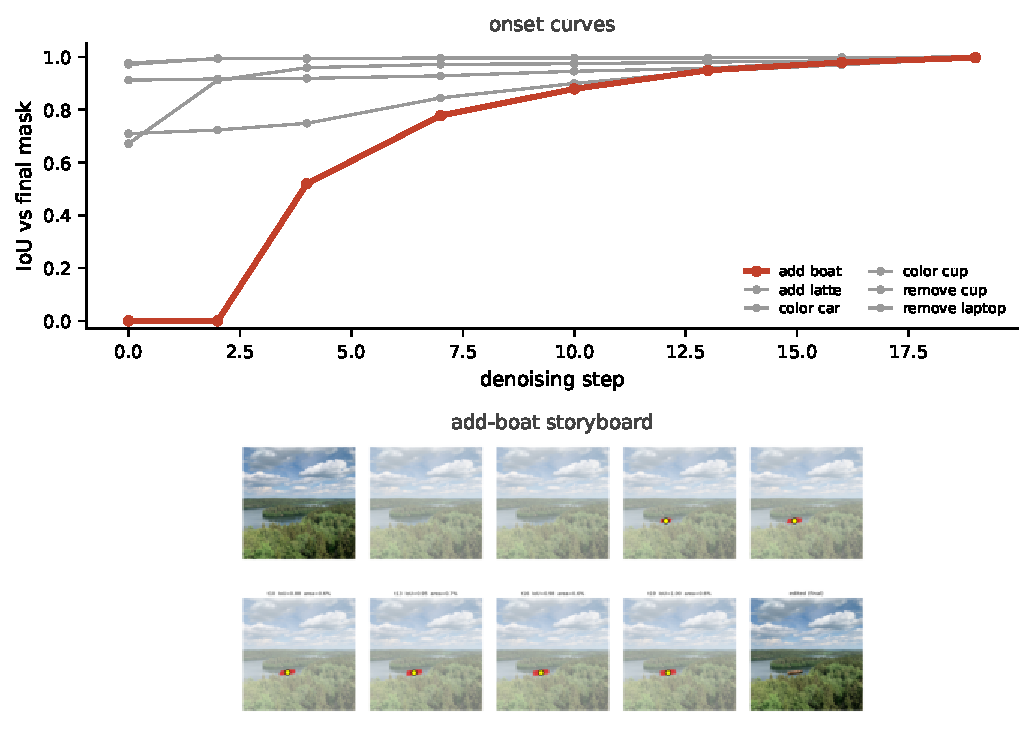
\includegraphics[width=\columnwidth]{figs/fig8_appendix/fig8_appendix.pdf}
  \caption{The self-correction case from \S\ref{sec:limits}. Top: IoU
  of the per-step edit mask against its final mask, for the 6
  non-global-edit battery cases. Five cases ("printing") are already
  $\ge0.67$ IoU at step 0; \emph{add\_boat} ("thinking") is entirely
  absent until step 4 and then grows to IoU $1.00$ by step 19. Bottom:
  the \emph{add\_boat} storyboard showing this growth happens
  \emph{in place}, not via relocation of an earlier draft.}
  \label{fig:onset}
\end{figure}

\paragraph{Tuned-lens fitting details.} For each cell (layer $\ell$,
timestep $t$) we collect paired examples $(h_i,v_i)$ from the
conditional pass -- the post-block residual $h_i\in\mathbb{R}^{3072}$
and the model's own ground-truth conditional-pass velocity
$v_i\in\mathbb{R}^{64}$ -- and fit $\hat v_{\ell,t}=W_{\ell,t}h+b_{\ell,t}$
by ridge regression, $\min_{W,b}\sum_i\lVert
v_i-(Wh_i+b)\rVert_2^2+\lambda\lVert W\rVert_F^2$, solved in closed
form after centering ($W_{\ell,t}=V^\top H(H^\top H+\lambda I)^{-1}$,
bias from the centering means). $\lambda$ is selected independently
per cell from the grid $\{10^{-4},10^{-3},10^{-2}\}$ on a held-out
$10\%$ split of the \emph{fitting} tokens (a random per-token split,
disjoint from the zero-shot test below); chosen values skew toward
$10^{-2}$ at shallow layers (L6--L44) and toward $10^{-4}$--$10^{-3}$
from L56 on. We fit $9$ layers ($6,12,24,36,44,48,52,56,59$) $\times$
$6$ steps ($0,2,4,8,12,16$) -- $54$ per-step dictionaries, plus $9$
pooled-over-$t$ dictionaries for a per-layer-only comparison -- a
coarse grid, not the full $60{\times}20$ cells. Training pairs come
from three source images, one per training family (\emph{remove\_cup},
\emph{beach\_background}, \emph{add\_boat}, i.e.\
\emph{remove}/\emph{background}/\emph{addition}): $4056$, $4056$, and
$4144$ target-grid tokens respectively, $12256$ pooled tokens per
per-step cell before the held-out split ($73536$ for a pooled-over-$t$
dictionary). The zero-shot evaluation (\S\ref{sec:tunedlens}) is a
second, coarser split than the one used to pick $\lambda$:
\emph{car\_red} ($4096$ tokens, the color family) is entirely absent
from the three training images, so held-out $R^2$ there tests
generalization to an unseen edit family and image, not merely unseen
tokens within a seen one.

\paragraph{Linear-probe fitting details.} The cross-seed probes
(\S\ref{sec:mechanism}, \S\ref{sec:families}) are
\texttt{sklearn.linear\_model.LogisticRegression} (multinomial,
\texttt{lbfgs}, \texttt{max\_iter=200}) at every cell, with
scikit-learn's default $L_2$ penalty ($C{=}1$) and no per-cell or
global regularization sweep -- unlike the tuned lens's per-cell
$\lambda$, the probe's regularization is fixed throughout. Each patch
token is its own training example (no pooling), restricted to the
edit-relevant region: the car's bounding box ($792$ patches) for the
color probe of \S\ref{sec:mechanism} ($N{=}3{\times}792{=}2376$ per
split per cell, an $11$-layer $\times$ $5$-step grid), and a
family-specific region for the four-family probes of
\S\ref{sec:families} (whole-frame, subsampled, for style; the
bounding-box complement for background; the bounding box itself for
removal and addition), swept over $5$ layers $\times$ $3$ steps per
family. The train/test split is by \emph{seed}, not token or image: fit
on hidden states from a run at seed $0$, evaluated on an independently
sampled run at seed $1$, same source image and prompt throughout -- so
a probe cannot simply memorize a seed-specific noise pattern.

These patch-token probes are basis diagnostics for the \emph{requested}
prompt label; patches within one generation are not independent
experimental units, so their accuracy is not used as generation-level
inference. The fixed-prompt outcome studies instead mean-pool the frozen
edit-region rows so each generation contributes exactly one vector.
T3 uses car seeds 100--147; the pre-registered real-photo follow-up uses
mug seeds 200--247 and eye seeds 300--347; the tree replication uses
seeds 400--447; and the independent Boogu replication uses seeds
500--547. Circular hue targets are represented as
$(\cos 2\pi h,\sin 2\pi h)$ and fit with ridge regression under frozen
or nested regularization as specified in each preregistration. Matched
permutation tests use the same outer folds and fitting procedure for the
observed and permuted labels.

For held-out selection, T7 trains only on Boogu seeds 500--547 and tests
12 consecutive five-seed groups, seeds 700--759. T8 trains only on Qwen
tree seeds 400--447 and tests 12 groups, seeds 800--859, with target hues
$[0,90,180,270]$ degrees repeated three times. T10 regenerates Qwen car
training seeds 100--147 in the current environment and tests 12 groups,
seeds 900--959; its four targets are frozen training-hue quantiles before
any test artifact exists. Every candidate feature is captured by an
actual interrupted run; the chosen winner is then rerun to completion.
T7 uses exact Poisson-binomial inference for selected edit success. T8
and T10 use the exact lower tail of the sum of within-group ranks. Their
rank sums are respectively 14 and 24 over 12 groups, giving
$91/5^{12}=3.72736\times10^{-7}$ and
$2{,}105{,}506/5^{12}=0.00862415$.
Preregistrations, scripts, analyses, and montages are in
\texttt{experiments/t3\_implicit\_choice\_prereg.md},
\texttt{t4\_real\_photo\_replication\_prereg.md},
\texttt{t6\_boogu\_outcome\_prereg.md},
\texttt{t7\_boogu\_seed\_selection\_prereg.md},
\texttt{t8\_tree\_target\_selection\_prereg.md},
\texttt{t10\_car\_target\_selection\_prereg.md}, and the corresponding
\texttt{runs/t3--t10} directories in the artifact repository.

The anonymous code/data supplement contains the maintained lens and
intervention implementation, paper experiment scripts, preregistrations,
source images, compact JSON result records, and the pooled early features for
T7--T10. It omits third-party model checkpoints, multi-gigabyte completed
generations, and full per-token hidden-state captures; those can be regenerated
from the supplied scripts and public checkpoints.

\end{document}
